\documentclass{article}

\usepackage{fancyhdr}
\usepackage{extramarks}
\usepackage{amsmath,esint}
\usepackage{amssymb}
\usepackage{amsthm}
\usepackage{amsfonts}
\usepackage{tikz}
\usepackage[plain]{algorithm}
\usepackage{algpseudocode}
\usepackage{enumitem}
\usepackage{mathtools}
\usepackage{siunitx}
\usepackage{tikz}
\def\checkmark{\tikz\fill[scale=0.4](0,.35) -- (.25,0) -- (1,.7) -- (.25,.15) -- cycle;}
%\usepackage{hyperref}
\graphicspath{ {./images/}}

\usetikzlibrary{automata,positioning}

\newcommand*\VF[1]{\mathbf{#1}}
\newcommand*\dif{\mathop{}\!\mathrm{d}}


%
% Basic Document Settings
%

\topmargin=-0.45in
\evensidemargin=0in
\oddsidemargin=0in
\textwidth=6.5in
\textheight=9.0in
\headsep=0.25in

\linespread{1.1}

\pagestyle{fancy}
\lhead{\hmwkAuthorName}
\chead{Study Guide For 33-142 Summer 2018}
\rhead{Professor Ghosh}
\lfoot{\lastxmark}
\cfoot{\thepage}

\renewcommand\headrulewidth{0.4pt}
\renewcommand\footrulewidth{0.4pt}

\setlength\parindent{0pt}

%
% Create Problem Sections
%

\newcommand{\enterProblemHeader}[1]{
    \nobreak\extramarks{}{Problem \arabic{#1} continued on next page\ldots}\nobreak{}
    \nobreak\extramarks{Problem \arabic{#1} (continued)}{Problem \arabic{#1} continued on next page\ldots}\nobreak{}
}

\newcommand{\exitProblemHeader}[1]{
    \nobreak\extramarks{Problem \arabic{#1} (continued)}{Problem \arabic{#1} continued on next page\ldots}\nobreak{}
    \stepcounter{#1}
    \nobreak\extramarks{Problem \arabic{#1}}{}\nobreak{}
}

\setcounter{secnumdepth}{0}
\newcounter{partCounter}
\newcounter{homeworkProblemCounter}
\setcounter{homeworkProblemCounter}{1}
\nobreak\extramarks{Problem \arabic{homeworkProblemCounter}}{}\nobreak{}

%
% Homework Problem Environment
%
% This environment takes an optional argument. When given, it will adjust the
% problem counter. This is useful for when the problems given for your
% assignment aren't sequential. See the last 3 problems of this template for an
% example.
%
\newenvironment{homeworkProblem}[1][-1]{
    \ifnum#1>0
        \setcounter{homeworkProblemCounter}{#1}
    \fi
    \section{Problem \arabic{homeworkProblemCounter}}
    \setcounter{partCounter}{1}
    \enterProblemHeader{homeworkProblemCounter}
}{
    \exitProblemHeader{homeworkProblemCounter}
}

%
% Homework Details
%   - Title
%   - Due date
%   - Class
%   - Section/Time
%   - Instructor
%   - Author
%

\newcommand{\hmwkTitle}{Homework\ \#11}
\newcommand{\hmwkDueDate}{May 1, 2018}
\newcommand{\hmwkClass}{21-127 Concepts}
\newcommand{\hmwkClassTime}{Section A}
\newcommand{\hmwkClassInstructor}{Professor Ghosh}
\newcommand{\hmwkAuthorName}{\textbf{William Cen}}
\newcommand{\eqn}{\[
    \stcomp{(A \cup B)} = \stcomp{A} \cap \stcomp{B}
\]}

%
% Title Page
%

\title{
    \vspace{2in}
    \textmd{\textbf{Study Guide For 33-142 Physics 2}}\\
    %\normalsize\vspace{0.1in}\small{Due\ on\ \hmwkDueDate\ at 3:10pm}\\
    \vspace{0.1in}\large{\textit{\hmwkClassInstructor}}
    \vspace{3in}
}

\author{\hmwkAuthorName}
\date{}

\renewcommand{\part}[1]{\textbf{\large Part \Alph{partCounter}}\stepcounter{partCounter}\\}

%
% Various Helper Commands
%

% Useful for algorithms
\newcommand{\alg}[1]{\textsc{\bfseries \footnotesize #1}}

% For derivatives
\newcommand{\deriv}[1]{\frac{\mathrm{d}}{\mathrm{d}x} (#1)}

% For partial derivatives
\newcommand{\pderiv}[2]{\frac{\partial}{\partial #1} (#2)}

% Integral dx
\newcommand{\dx}{\mathrm{d}x}

% Alias for the Solution section header
\newcommand{\solution}{\textbf{\large Solution}}

% Probability commands: Expectation, Variance, Covariance, Bias
\newcommand{\E}{\mathrm{E}}
\newcommand{\Var}{\mathrm{Var}}
\newcommand{\Cov}{\mathrm{Cov}}
\newcommand{\Bias}{\mathrm{Bias}}

\begin{document}

\maketitle

\pagebreak
\section{General Knowledge}
What you should know (This doesn't include all the equations from the formula sheet, just the important ones):\\
\label{definitions}
\begin{description}
\item[Vectors]
Example: $\vec{E} = \frac{q}{4\pi\epsilon |r|^3}\vec{r}$\\
An abstract tool useful for physics. It has a direction and magnitude, so you can use vectors to describe anything that depends on direction, such as electric fields. 

\item[Unit Vectors]
Example: $\hat{r} = \frac{\vec{r}}{|\vec{r}|}$\\
A vector with magnitude 1. This is quite important when describing direction. In fact, our definition of the electric field above can be condensed to: $\vec{E} = \frac{q}{4\pi\epsilon r^2} \hat{r}$

\item[The "r" vector]
Just a vector describing radial direction. Conveniently, this is also $\vec{r} = r <cos(\theta), sin(\theta)>$

\item[Coulomb (C)]
SI unit of measurement for charge

\item[Epsilon ($\epsilon$)]
Constant of dielectric permitivity. Larger epsilons lead to smaller magnitudes of electric fields.

\end{description} 

\subsection{Useful Constants}
$Q_{\text{proton/electron}} = \pm1.60 * 10^{-19} \text{C}$\\
\\
$\frac{1}{4\pi\epsilon_0} = 8.99 * 10^9 N\cdot m^2 \cdot C^{-2}$ Note that $\epsilon_0$ is used here because this refers to the constant of dielectric permitivity in a vacuum (which we will frequently use) \\
\\
$\hat{i}, \hat{j}, \hat{k} = $ x, y, z unit vectors: $<1,0,0>, <0,1,0>, <0,0,1>$
\subsection{Important Concepts}
\textbf{Coulomb's Law}: $\vec{F}_{\text{Coulomb}} = \frac{1}{4\pi\epsilon} \frac{Q_1 Q_2}{|r|^2} \hat{r}$\\
\\
\textbf{Superposition Principle}: A principle that describes that the net effect at a point in space is the net sum of all the individual effects from all sources at that point. This can be simplified to our description of electric fields. The net electric field at a point is the sum of all individual electric fields at that point: $\vec{E}_{net} = \sum\limits_{i}\vec{E}_i$.\\
\\
\textbf{Conservative System}: In a conservative system, all energy is conserved. This also means that there are no external forces involved, since the source and effect is all contained within the system. For example, a system that has 2 charges and only has the fields due to those two charges is conservative. However, if you enclose the effects of both but only one of those charges, then the electric field due to the charge not in your system is an "external" effect.\\

\subsection{Useful Equations}
\textbf{Dot Product}: Say $\vec{u} = <u_x, u_y>, \vec{v} = <v_x, v_y>$, then  $\vec{u} \cdot \vec{v} = u_x*v_x + u_y*v_y = |\vec{u}||\vec{v}|cos(\theta)$ \\
\\
\textbf{Cross Product}: Say $\vec{u} = <u_x, u_y, u_z>, \vec{v} = <v_x, v_y, u_z>$, then 

\[
\vec{u} \times \vec{v} =
    \begin{vmatrix}
        \hat{i} & \hat{j} & \hat{k} \\
        u_x & u_y & u_z \\
        v_x & v_y & v_z \\
    \end{vmatrix}
= (u_y v_z - v_y u_z)\hat{i} - (u_x v_z - v_x u_z)\hat{j} + (u_x v_y - v_x u_y)\hat{k}
\]
The magnitude of the cross product is given as $|\vec{u} \times \vec{v}| = |\vec{u}||\vec{v}|sin(\theta)$ \\
\\
\textbf{Magnitude of vector}: Say $\vec{v} = <v_1, v_2, v_3, v_4, ... v_n>$. Then, $|\vec{v}| = \sqrt{v_1^2 + v_2^2 + v_3^2 + ... v_n ^2}$\\
\\
\textbf{Taylor Expansion of Power Series (Binomial Expansion)}: $(1 + x)^\alpha = 1 + \alpha x$ when $x << 1$
\pagebreak

\section{Vectors!}
So one of the most important and useful concepts in many fields, most notably physics and mathematics, is the concept of vectors. When we call something a vector $\vec{v}$, then we mean that "v" has both a magnitude, or value like speed, and direction. Basically, we give this vector a length, or value, equal to the value of "v". Here comes to play another extremely important concept in vectors. That is, since a vector is just an arrow, we can describe this vector using 2 other perpendicular vectors. This is called "decomposing" a vector. There are infinitely many ways to decompose a vector, which allows us to deal with so many situations, such as a gravitational force vector decomposed along the inclined plane. Generally, we like to represent our vectors in the Cartesian plane, or $<x_\text{val},y_\text{val}>$. \\
\begin{figure}[!h]
\center
    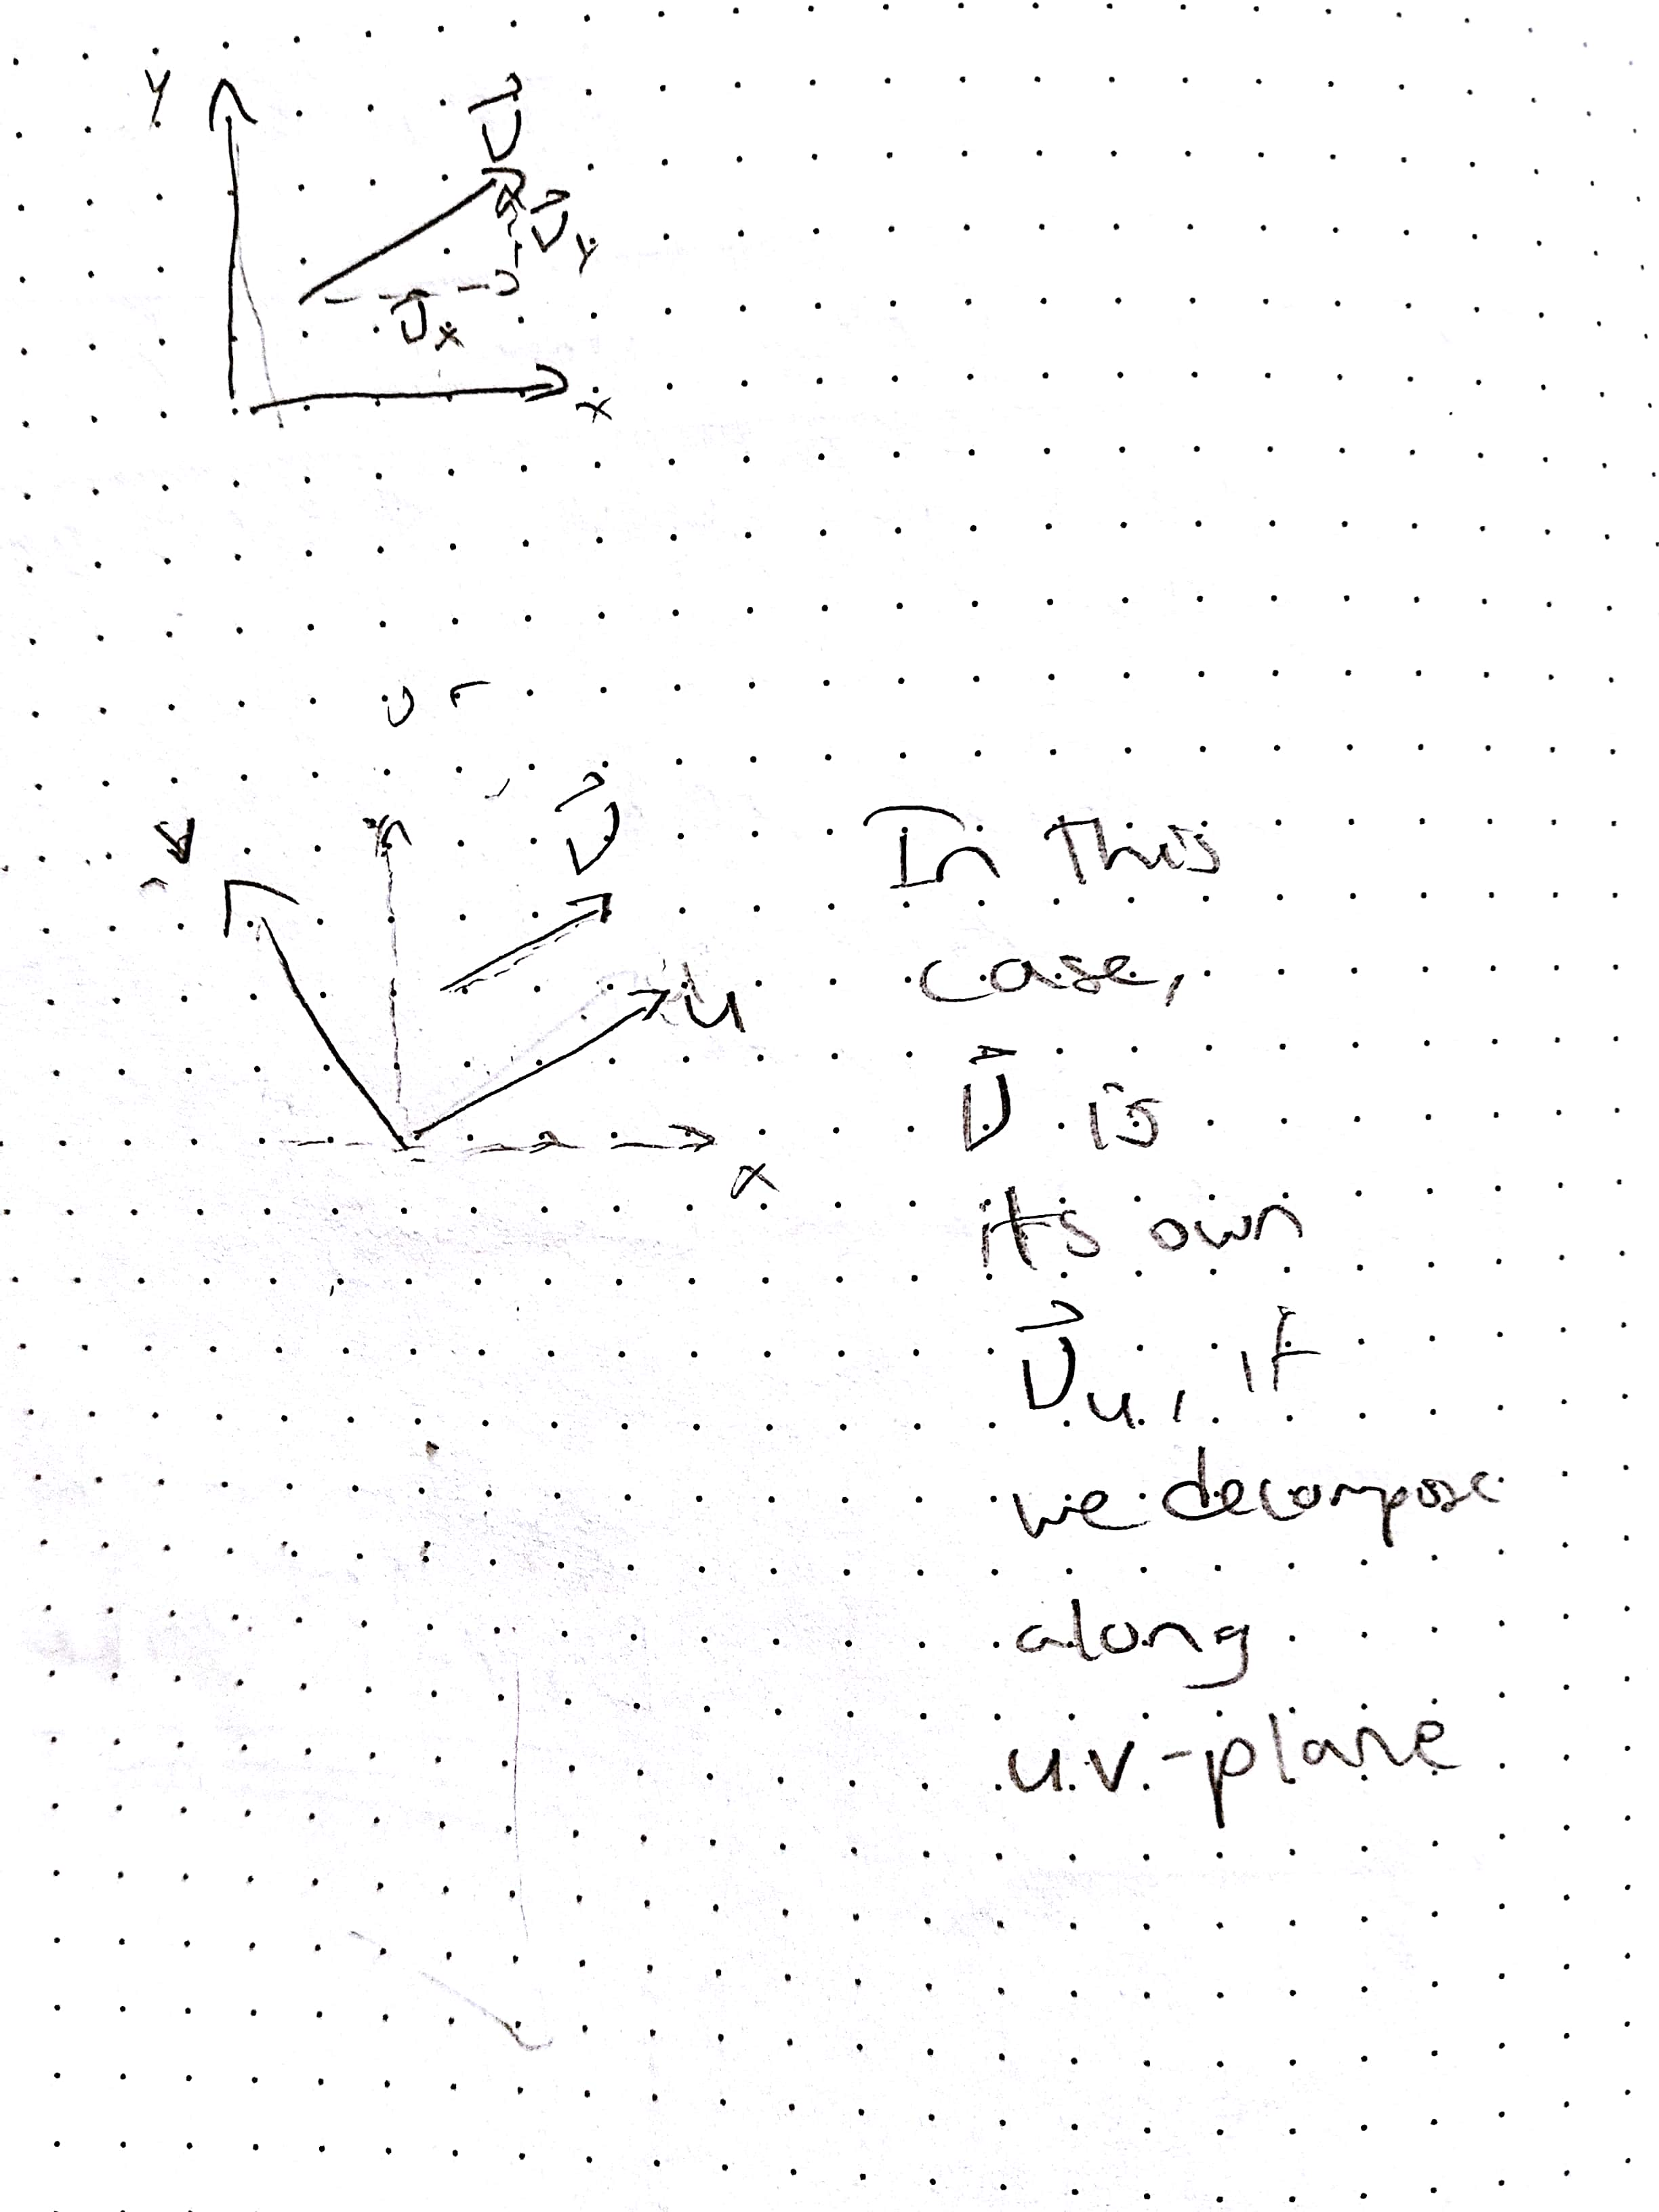
\includegraphics[width=.4\textwidth]{Vectors1.jpg}
    \caption{This image represents how you can decide whatever plane you wish to decompose the vector along. It's important to recognize that the uv-plane can be any arbitrary plane.}
\end{figure}
\\
\\
Now suppose I have some arbitrary vector that I know the magnitude of and direction of. But, consider I only know the direction is 30 degrees north of the positive x axis. This means that my vector should have a 30 degree angle with the x axis and it should point diagonally up-right. So, we have a vector pointing in this direction. Now, if you recall from trigonometry, we can decompose this vector so that we have an x and y component. With a 30 degree angle with the x axis, our x component is like the base of the triangle, or $\text{val}*cos(\ang{30})$. Then our y component is $\text{val}*sin(\ang{30})$. Then, we can represent a vector as its x and y components, as mentioned at the end of the first paragraph: $\vec{V} = <V cos(\theta), V sin(\theta)>$. You may see another notation: $\vec{V} = V cos(\theta) \hat{i} + V sin(\theta) \hat{j}$.\\
\\
Another important concept in vectors is the notion of a vector field. To put it simply, you can imagine some field, say the xy-plane, and at each position, you have a different vector. In physics, we have gravitational fields and electric fields. These can be represented in many ways, most notably by using $r$ such as in $\vec{E} = \frac{1}{4\pi\epsilon}\frac{Q}{|r|^2}\hat{r}$. You can also represent this in the xy-plane by $\vec{E} = \frac{1}{4\pi\epsilon}\frac{Q}{x^2+y^2} <\cos{\theta}, \sin{\theta}>$. These are vector fields. There is the general form of each vector (the equation), but depending on the point in space you choose, you have a different value when you calculate the vector. Then, a vector field, visually, is when you show the vectors at every point in space:  

\pagebreak

\section{Verification and Approximation}
In physics, an extremely important issue when dealing with new equations or formulae is the necessity to be able to verify its validity. However, if an equation is not immediately clear, there are several ideas that we apply within electricity and magnetism to understand an equation. These are all incorporated within the context of the next section.
\subsection{Does it Make Sense?}
The idea of whether or not an equation makes sense is quite general. But, you should know several ideas when approaching this question. One is utilizing dimensional analysis. This is a useful tool because if your equation does not have the right units, it clearly cannot be correct. By representing each variable as its SI unit form, you can perform the dimensional analysis:\\
\\
Example:
\begin{align*}
	\vec{E} =& \frac{1}{4\pi\epsilon}\frac{2Qd}{|r|^3}\hat{r}\\
	=& \frac{(C)^1(m)^1}{m^3}\\
	=& (C)^1(m)^1(m)^{-3}\\
	=& (C)^1(m)^{-2} \ \ \ \checkmark \text{Verified}
\end{align*}\\
So, clearly, the equation for the dipole electric field (along axis) surely holds correct units. At this point, one may think that it is more beneficial to just verify it by re-deriving the equation. However, there are several issues with this. One, it is not always true that you will encounter easily-derivable equations. In addition, deriving an equation can still lead to errors, which will not change the issue. \\
\\
Following this, let us discuss the next method of evaluation. In physics, especially electricity and magnetism, the use of extremeties is a great way of understanding the equation's validity. This is because while we cannot necessarily understand the more complex picture, by going to extremities such as $\infty$, we can visualize and make sense of an equation.\\
\\
Example:
\begin{equation*}
	\vec{E}_{\text{ring}} = \frac{1}{4\pi\epsilon}\frac{Q}{2\pi R}\frac{2\pi R z}{(R^2 + z^2)^{3/2}}\hat{z}
\end{equation*}\\
At first, the ring equation is very hard to visualize or interpret. However, let us imagine condensing the ring into a singular point, then it should behave as a point charge. In our equation, this means we let the radius $R$ approach $0$.\\
\begin{align*}
	\vec{E}_{\text{ring}} &= \frac{1}{4\pi\epsilon}\frac{Qz}{(0 + z^2)^{3/2}}\hat{z}\\
	&= \frac{1}{4\pi\epsilon}\frac{Qz}{z^3}\hat{z}\\
	&= \frac{1}{4\pi\epsilon}\frac{Q}{z^2}\hat{z} \ \ \ \checkmark \text{Verified}
\end{align*}

\pagebreak

\section{Superposition Principle}
The superposition principle is one of the most beautiful concepts in physics. It is very hard to convey just how amazing and versatile it is without some examples. To begin with, the simple idea of the superposition principle (Let us discuss this in the context of an electric field for simplicity sake) is that net electric field at any point is the sum of all individual electric fields at that point:\\
\begin{equation*}
	\vec{E}_{\text{net}} = \sum\limits_{i} \vec{E}_i
\end{equation*}\\
This also applies to other ideas such as charges:\\
\begin{equation*}
	Q_\text{Total} = \sum\limits_{i} Q_i
\end{equation*}\\
Now charges are not exactly vectors, but charges emanate electric fields, so the sum of all charges should be the total charge. Now, we can demonstrate just how beautiful the superposition principle is. Consider a very convoluted problem: I have a circle of uniform charge distribution $\sigma$ but I cut out 2 adjacent holes in it. What is my electric field along the x axis?\\
\begin{figure}[ht]
\center
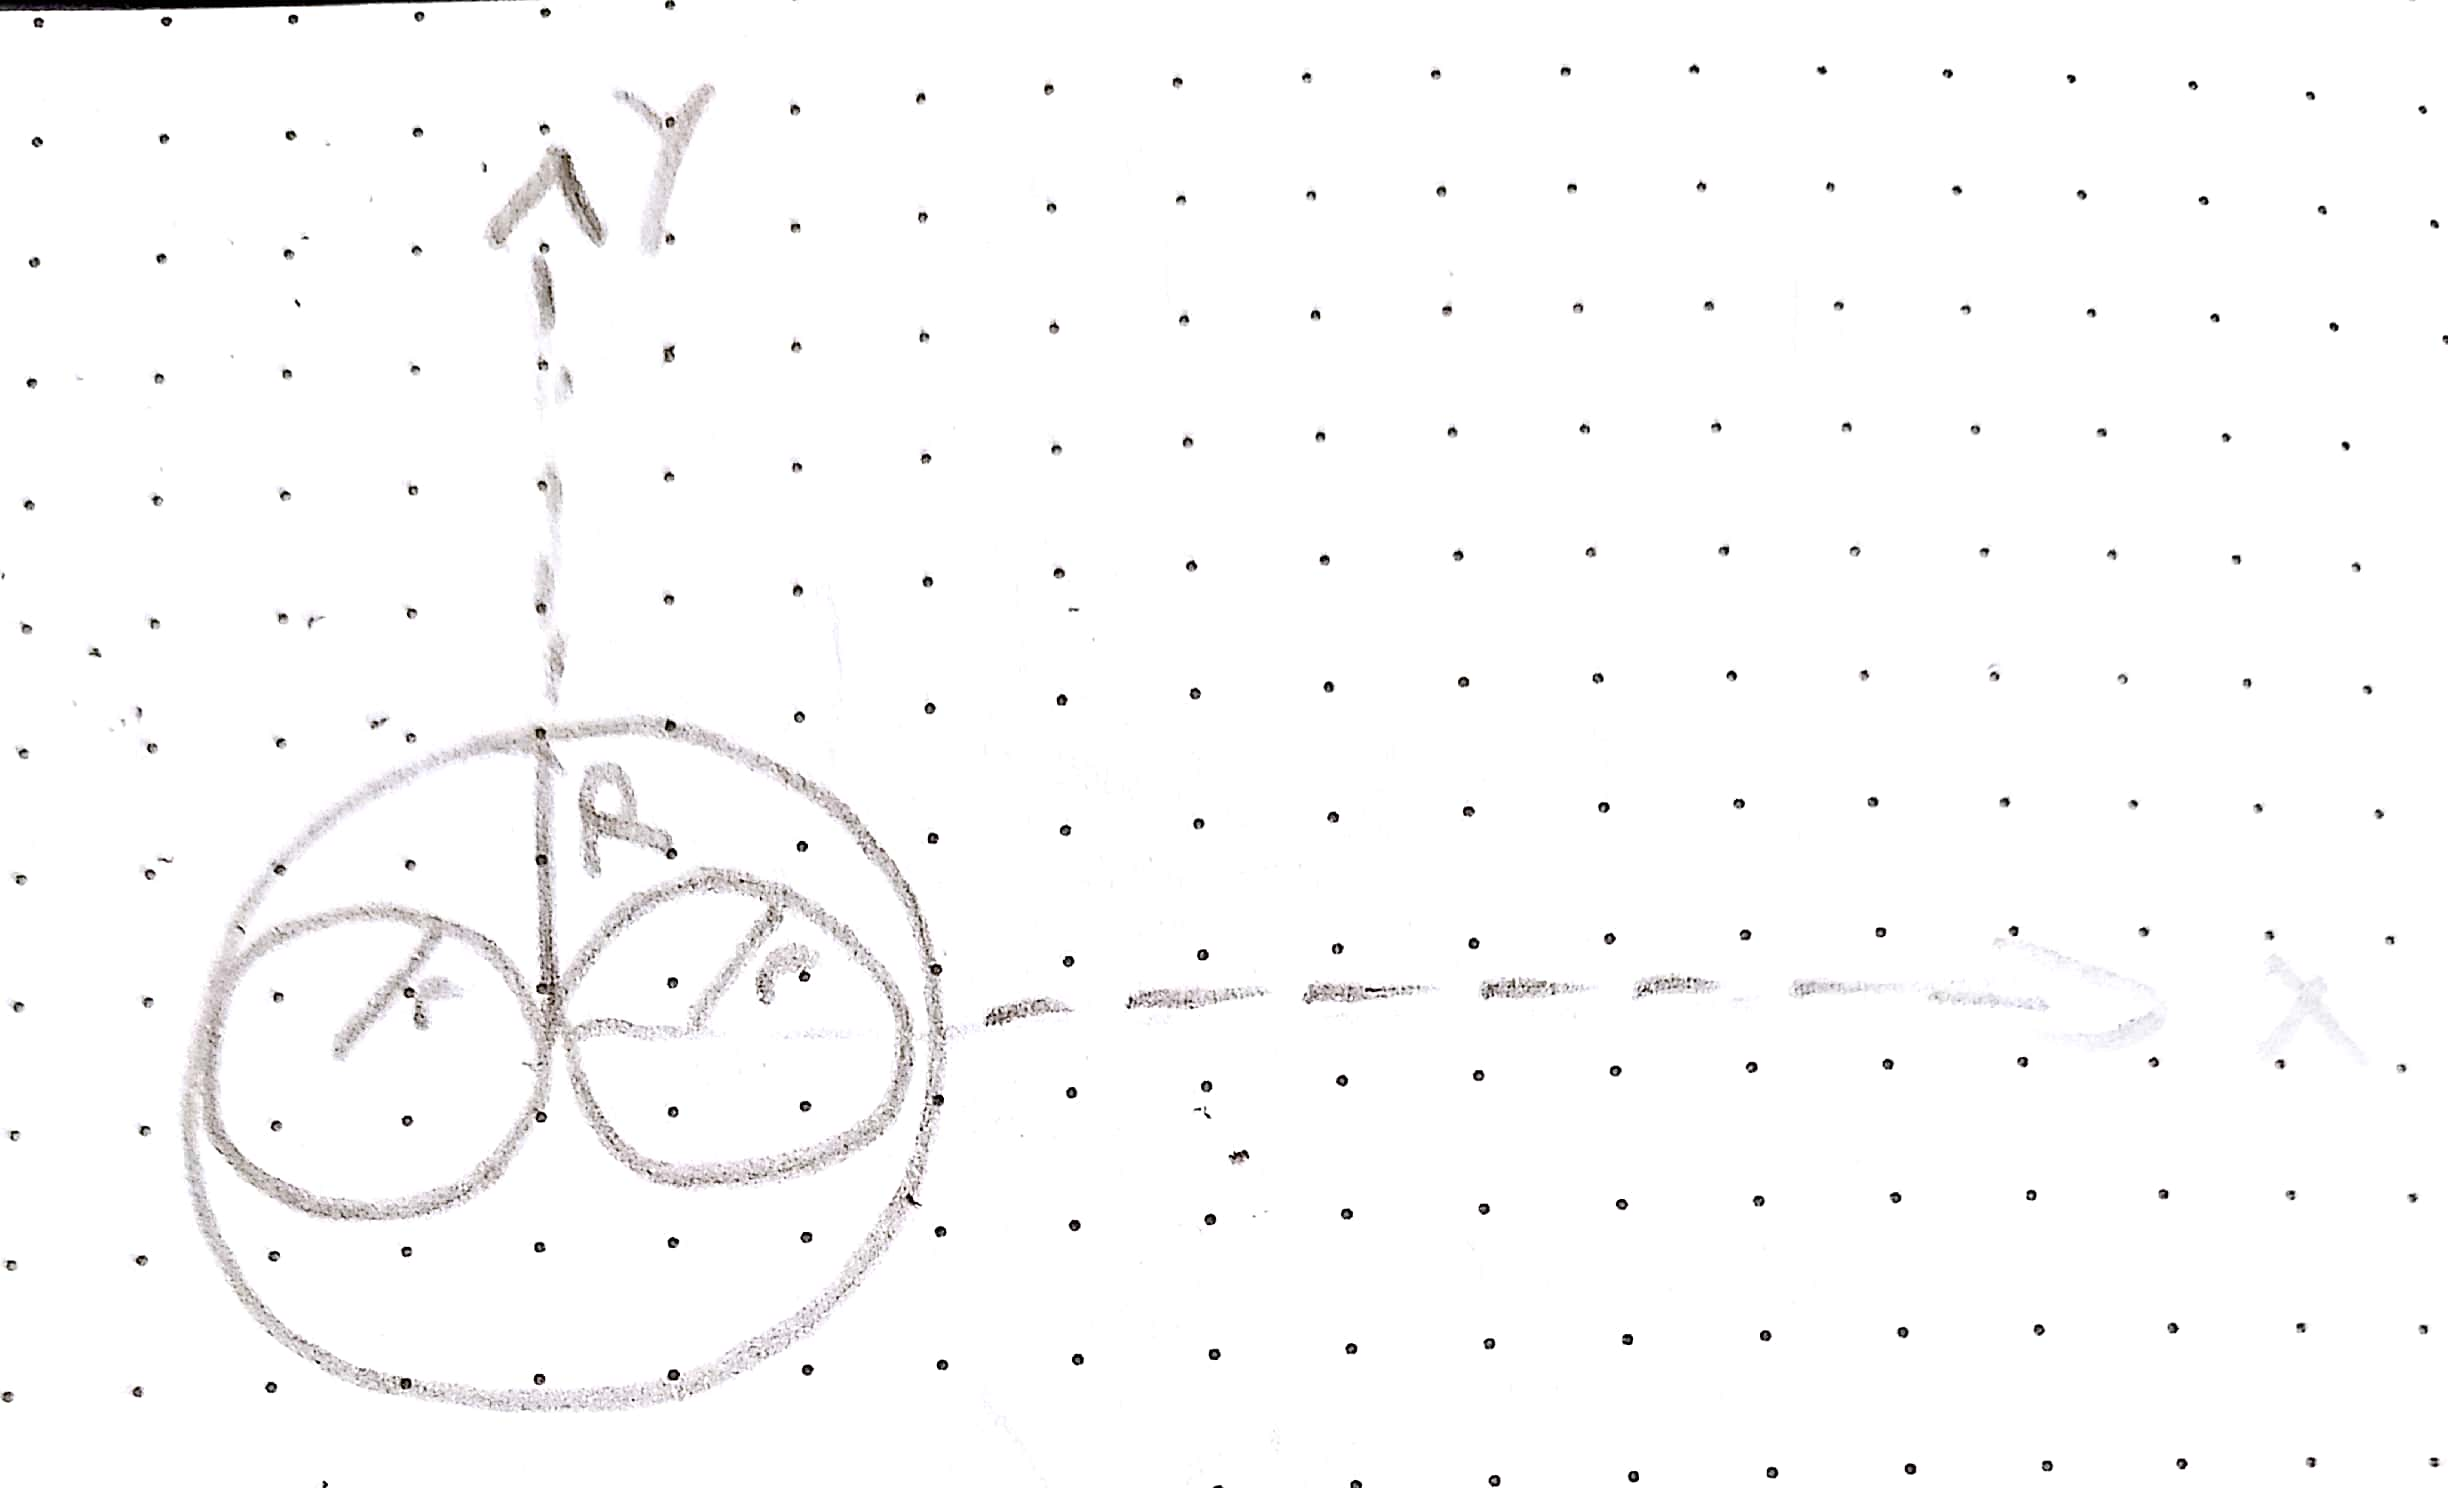
\includegraphics[width=.4\textwidth]{Superposition1.jpg}
\caption{A visualization of the problem. The inner holes are of radius r, and the rest of the circle is filled with charge.}
\end{figure}\\
\\
On its own, this problem may seem beyond the scope of our understanding. There is symmetry, but it is very convoluted. However, we know that the empty circles technically have 0 charge and the rest as some charge based on our charge density. So, we utilize our idea in the superposition principle. The effects at any point is the sum of all the effects. Now, we have 0 charge in the holes. Alone, this shape is hard to integrate over. But, we can imagine this shape as the sum of a full circle of positive charge and the sum of 2 smaller circles of negative charge. Why can we do this? Let us explain through the charge interpretation. It is as if we are adding positive charge in those circles. But at the same time, we are getting rid of those charges by creating 2 circles of negative charge (equal and opposite). So, our superposition principle says we still have the same situation.\\
\pagebreak
\begin{figure}[ht]
\center
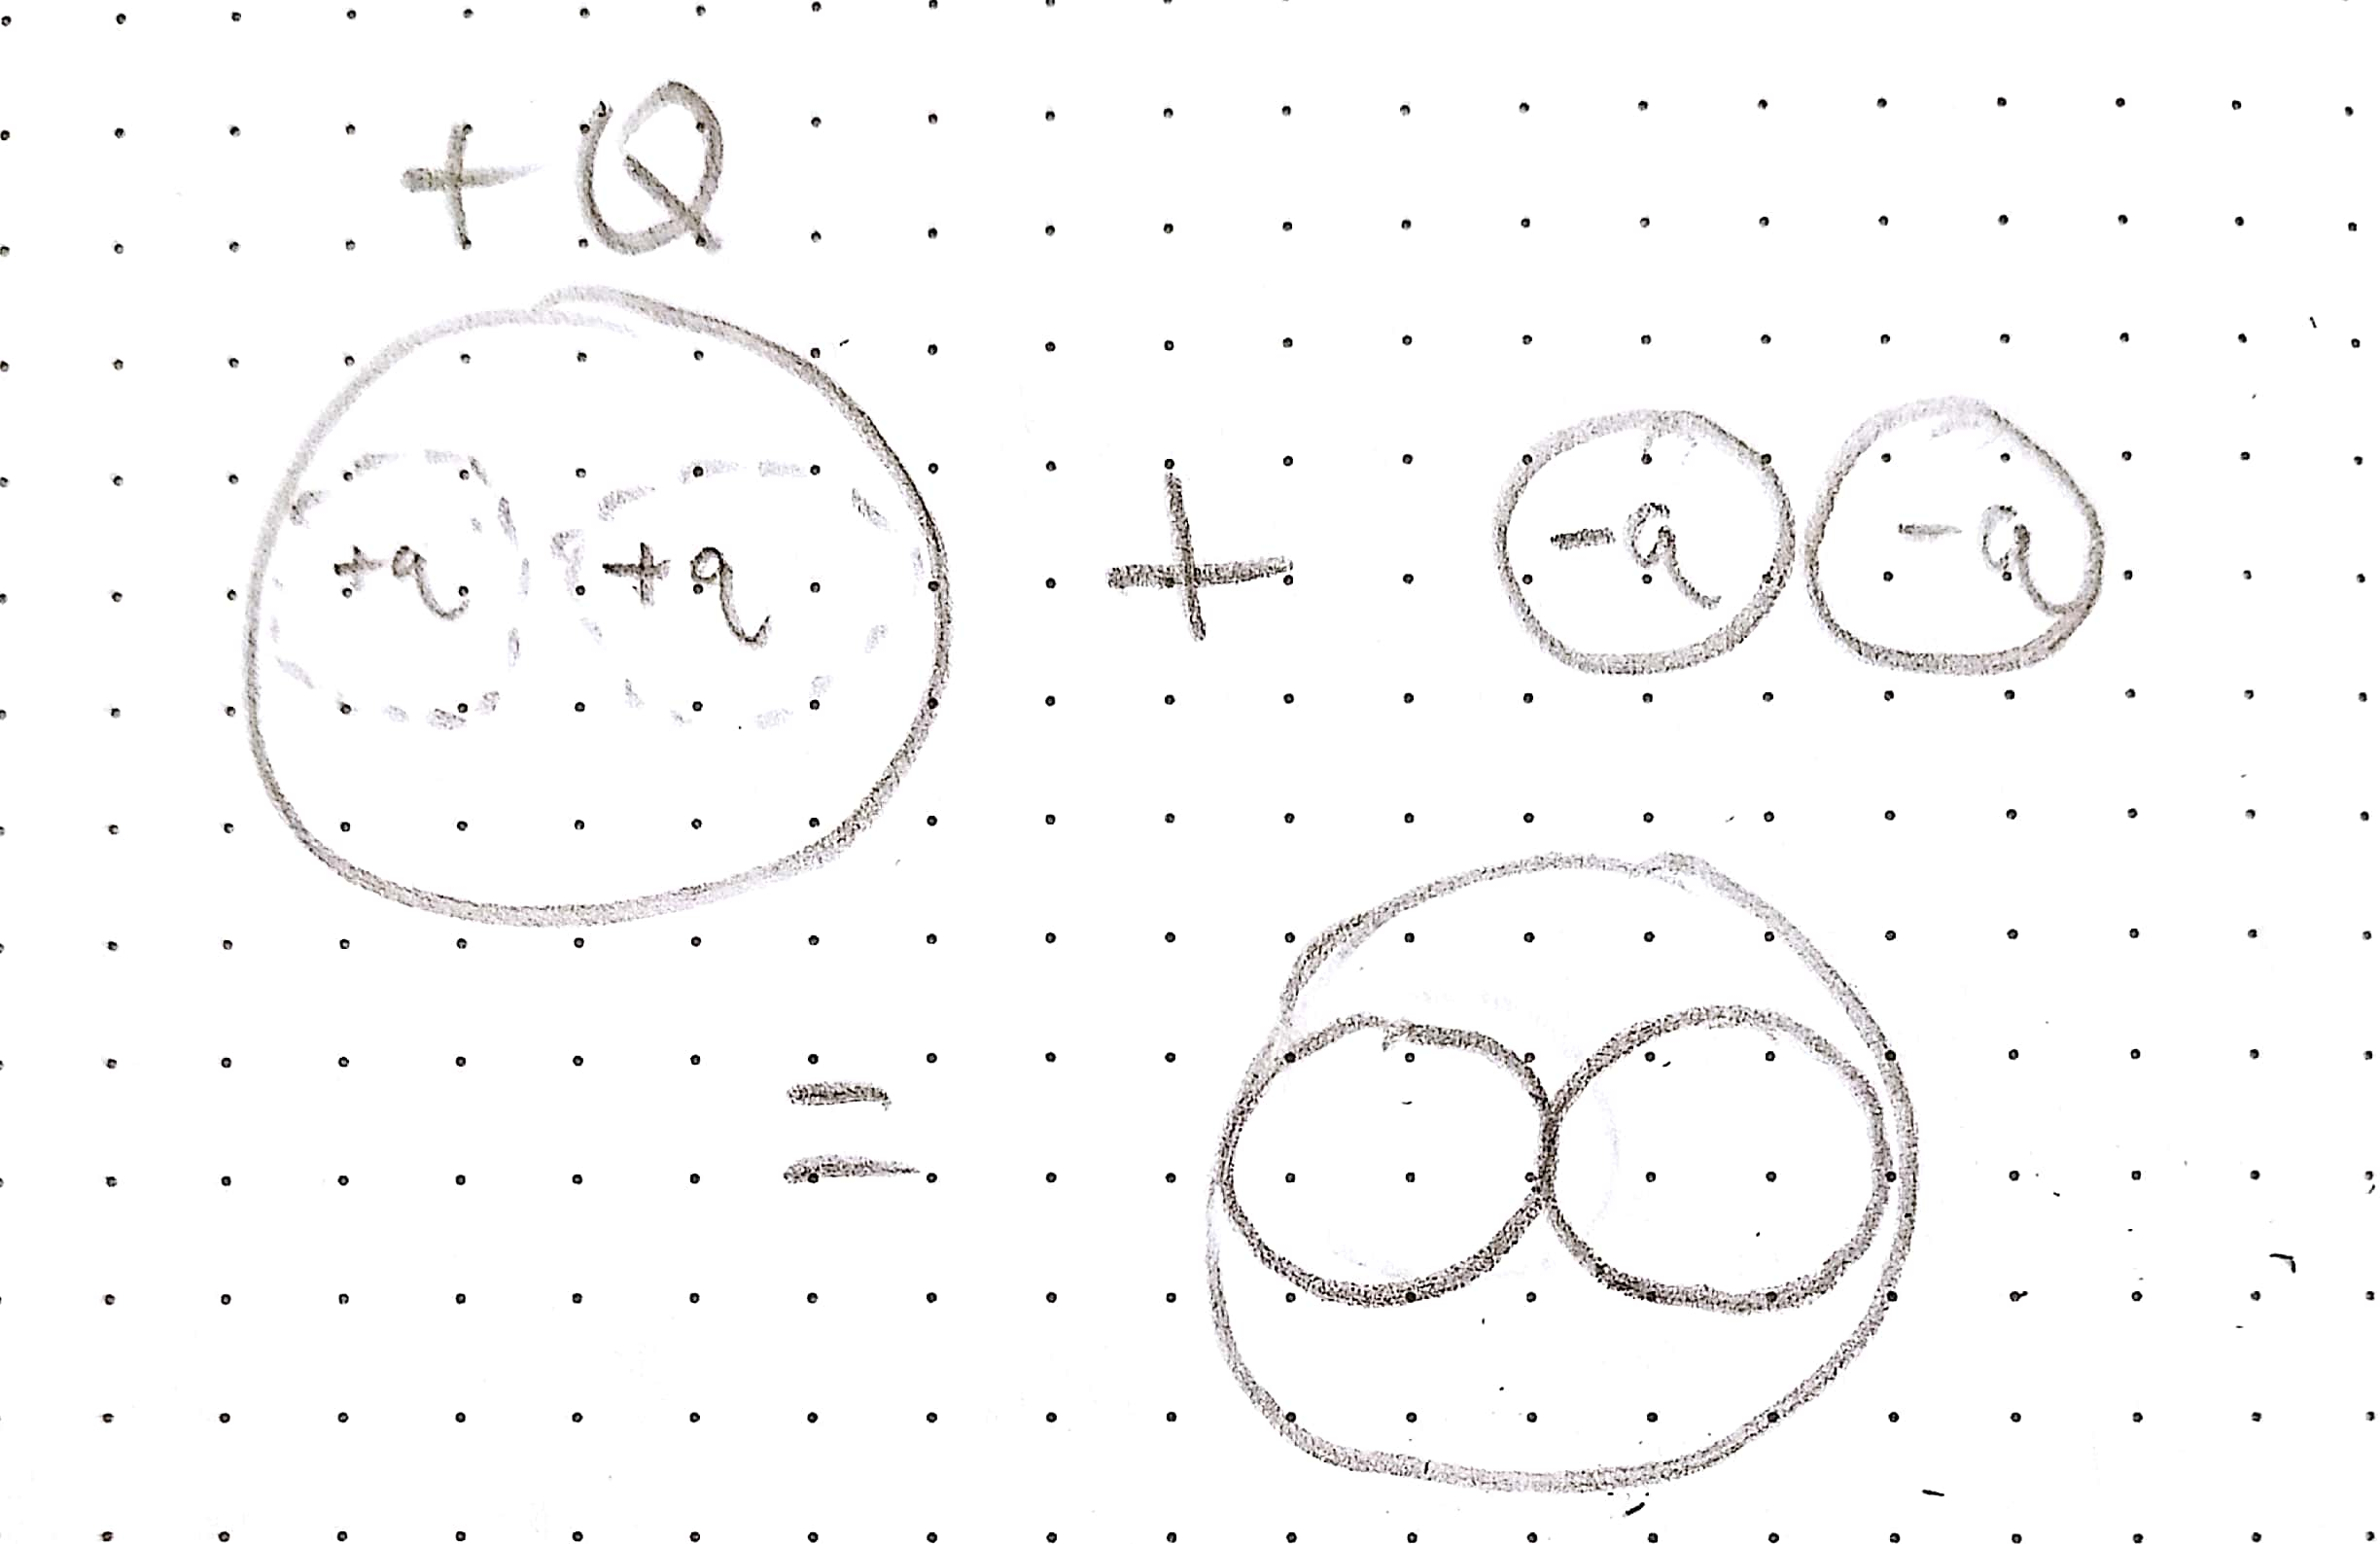
\includegraphics[width=.4\textwidth]{Superposition2.jpg}
\caption{We can understand the holes as just being occupied simultaneously by equal and opposite charges. So, combining the positive charges with the uniform density, we have a full circle and combining the negative charges of the same density, we have 2 negatively charged circles.}
\end{figure}\\
So all you do is just add the electric field from the circle plus the electric field from the negative circles (position in space still matters, so it's not simply 2 times a negative circle's electric field centered at the origin). But just notice how beautifully superposition principle allows us to approach problems. 

\pagebreak
\section{Week 1: Charges and Fields}

If you wish to just learn the equations and general concepts, I'd recommend just the first page of this study guide, since it provides that. If you wish for important concepts that will aid you in thinking, then the Week by Week pages will be useful. I should have a section on vectors if that is a concept you wish to review. \\
\\
Primarily, let us quickly discuss the importance of understanding the concept of an electric field. While Coulomb's Law is also very important, an important concept that arises from this class is the concept of fields. As Ghosh said, if previously there was no charge, but suddenly there is, there is suddenly a changing of the space around it. When I say the space changes, I mean that there is a field that other charged particles in the space will feel effects from. So, when we talk about the Coulomb field, we talk about the field due to a charged particle. And just like the gravitational field, electric fields due to singular charges are radial.\\
\\
\textit{Interesting question: If I have 1 charge then suddenly introduce another charge a light year away, would the effect of the distant charge be instantaneous or take time? If it takes time, how long should it take?}\footnote{Electric fields are essentially a result of travelling photons, so we should expect it to take 1 year for our charge to experience the effect of the distant charge}\\
\\
Recall that we learned what an electric field is $\vec{E}$ and Coulombs Law, $\vec{F}_{\text{Coulomb}} = \int \vec{E} \dif q$. This notation is simply restating the idea of the superposition principle. In fact, we can describe $\vec{E} = \frac{1}{4\pi\epsilon} \int \frac{\dif q}{|r|^2} \hat{r}$. When we say  $\vec{E} = \frac{1}{4\pi\epsilon} \int \frac{\dif q}{|r|^2}\hat{r}$, we are saying that what is the net electric field at this point due to all charges. However, in order for the integral to be practical, you should generalize the form. This is quite useful for more convoluted problems. However, when you deal with physical point charges, it's more useful to utilize the general principle (superposition): $\vec{E}_{\text{net}} = \sum\limits_{i} \vec{E}_i$. This is why you shouldn't ever need to use an integral to deal with problems like Ghosh's example: 4 charges are placed at the edges of a box, and find the force on the charge at the bottom left corner (Which can either be envisioned as the force on that charge due to each of the other charges in the box or the net electric field due to the other charges in the box times the charge you care about).\\
\begin{figure}[ht]
\center
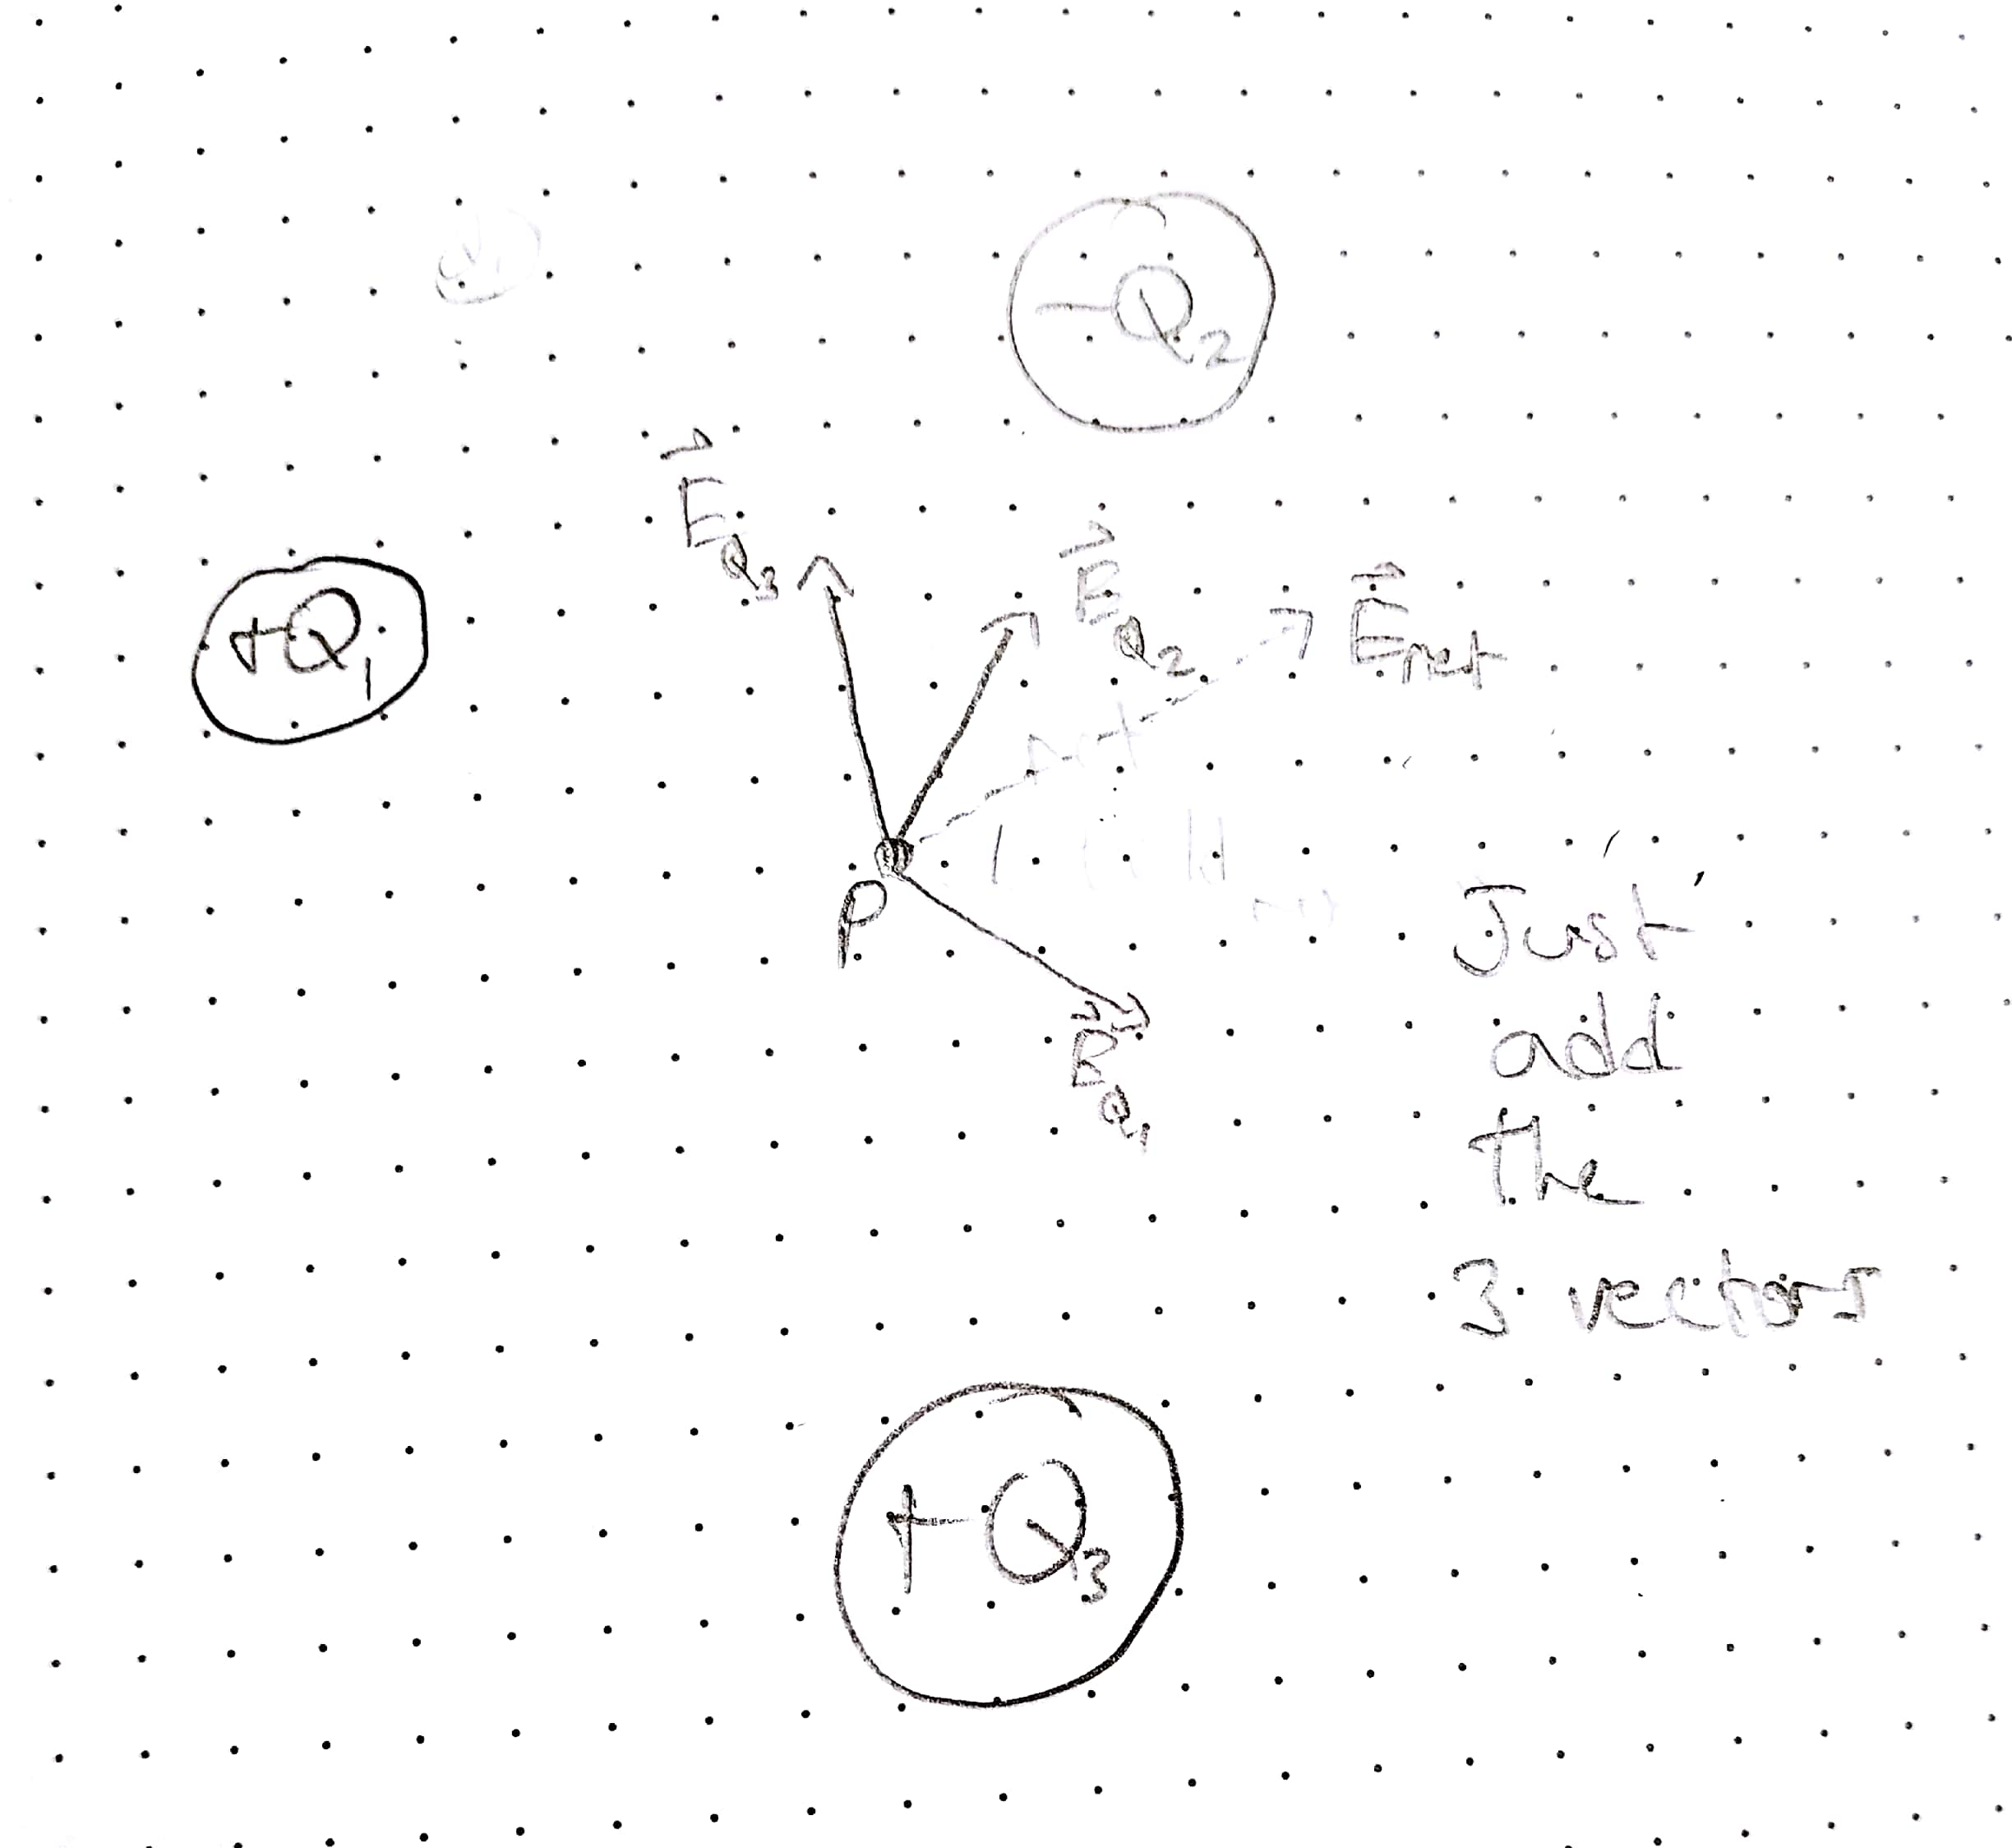
\includegraphics[width=.4\textwidth]{Vectors2.jpg}
\caption{This image represents the idea of superposition. As you can see, the electric field at any point can be represented by the sum of the electric field of every individual electric field at that point (in this case, the sum of electric fields due to individual charges).}
\end{figure}\\
\\
\subsection{Extra Mini Subsection: Dipoles}
Another very important concept in physics is the concept of a dipole. Why is this important? Well, as you'll later learn, many induced charge distributions in materials can be generalized to be a dipole, which tremendously simplifies the problem. In physics, we aim to turn something convoluted into something very simple and beautiful. Now, for a dipole, the general question is, how do I determine the electric field of a dipole. What's even more interesting is that the net charge of a dipole is 0 Coulombs, since there is a positive and negative charge contained in a dipole. However, even still, there should still be a net electric field. To calculate this, we apply the superposition principle again. Calculate the electric field due to one charge and add it to the electric field due to the other charge. For the purposes of this class, we only should be able to determine the electric field along the dipole's axis and the electric field along the perpendicular axis stemming from its midpoint.\\
\begin{figure}[ht]
\center
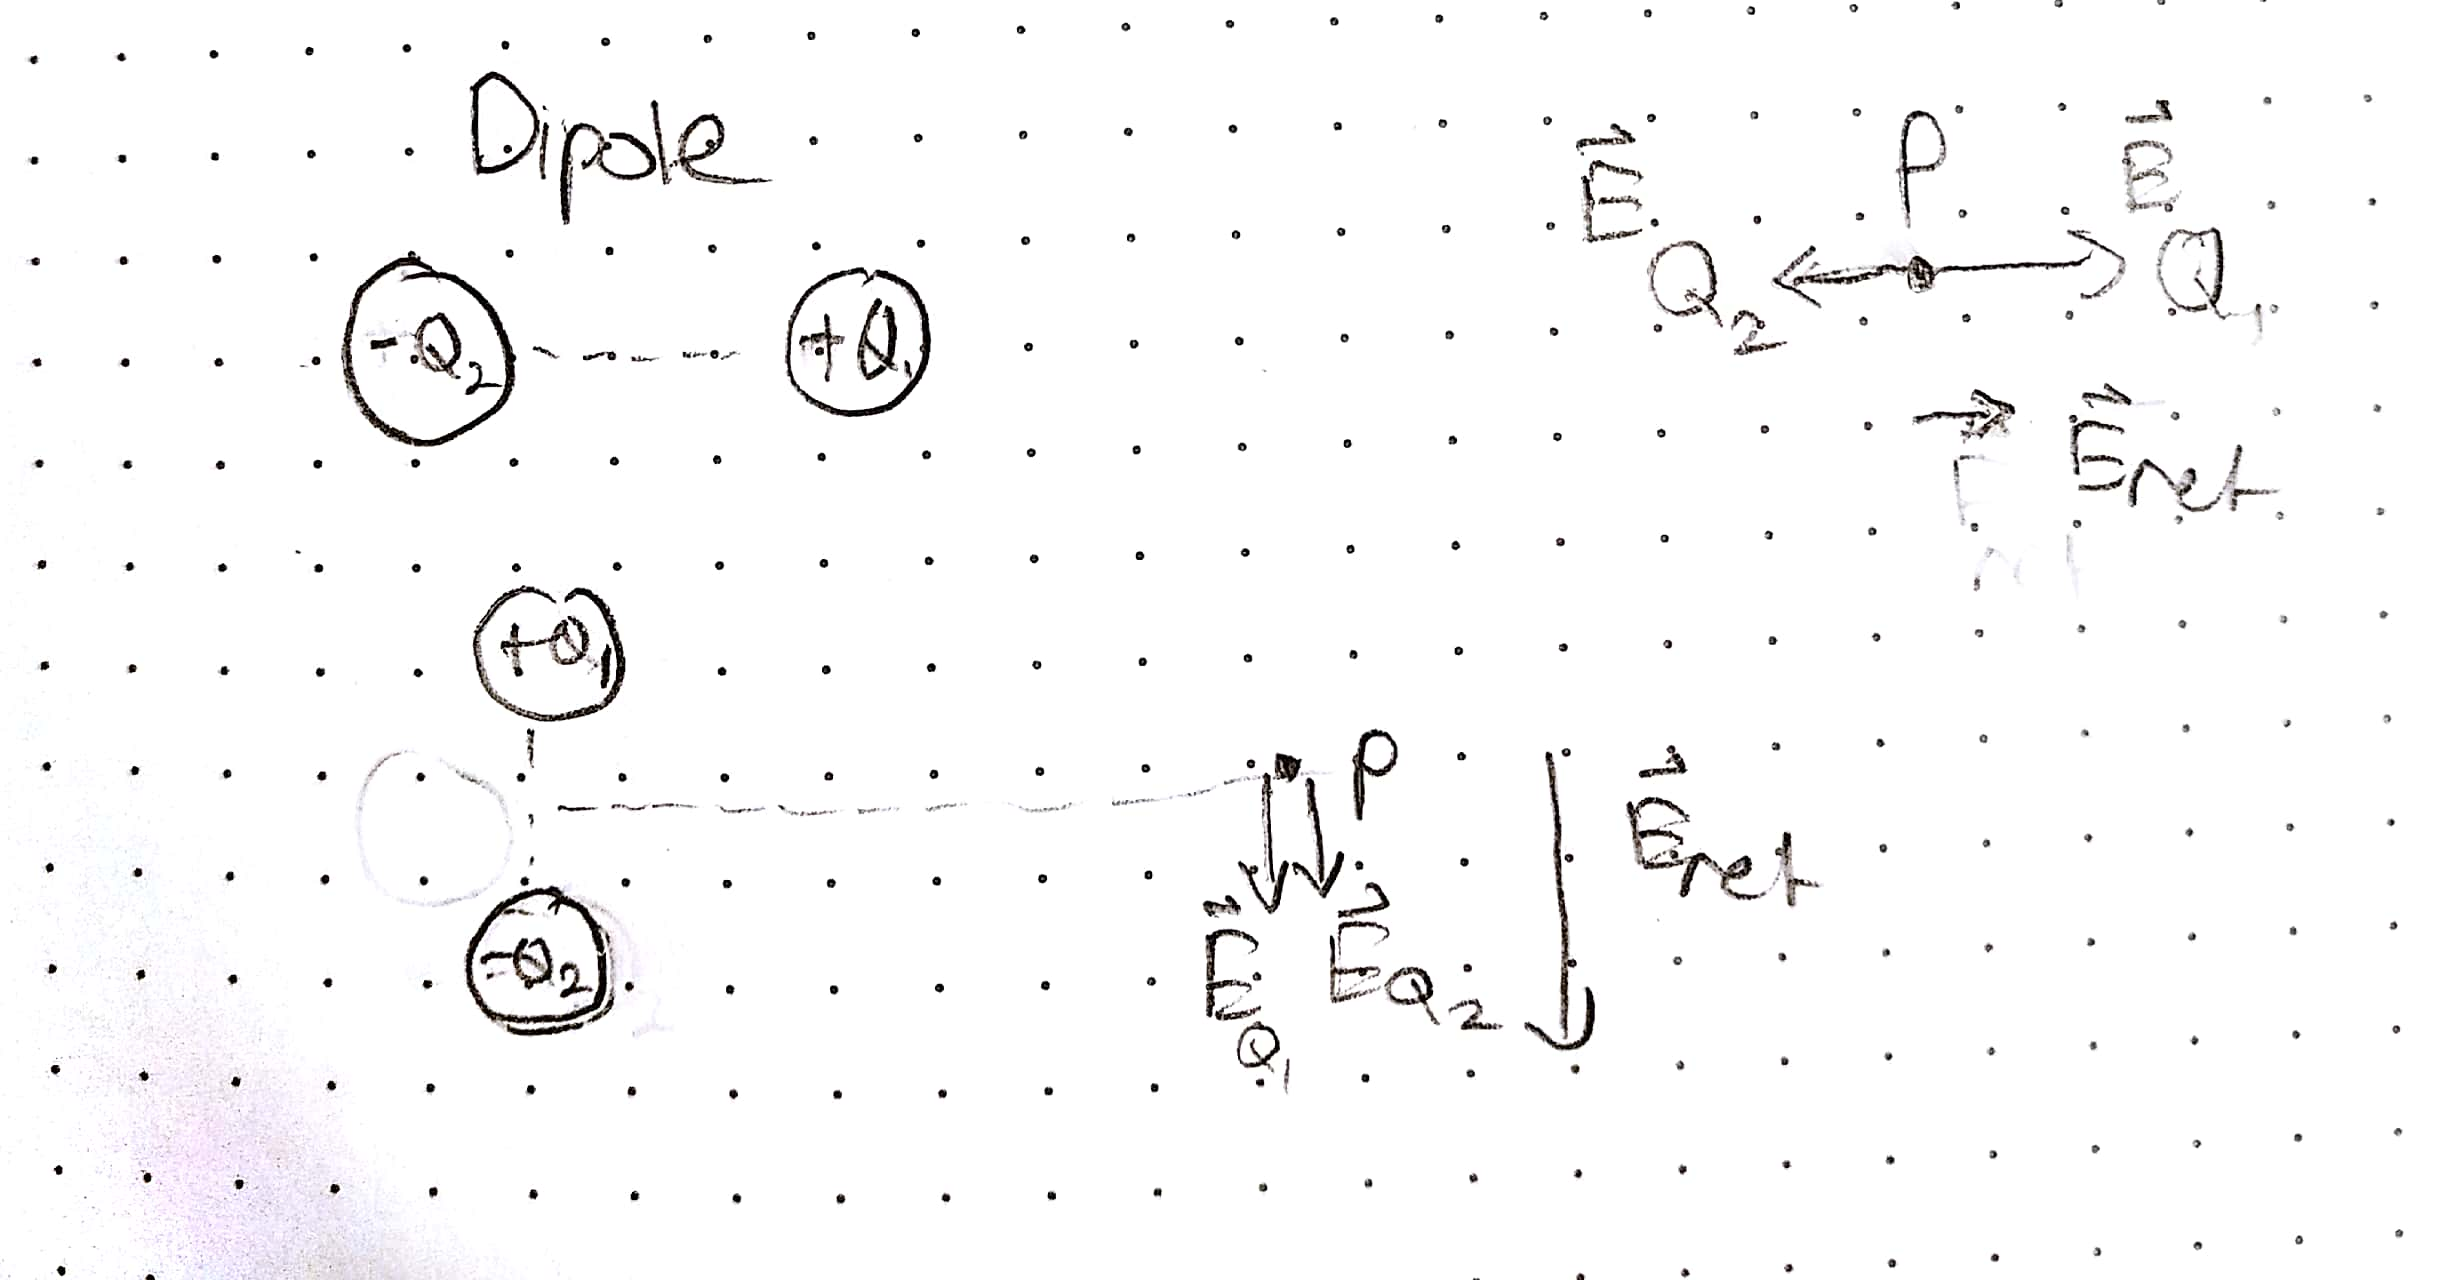
\includegraphics[width=.4\textwidth]{images/Week1pic2.jpg}
\caption{This image demonstrates the general idea you should have when deriving the electric field due to a dipole.}
\end{figure}\\
\\
So, let us proceed by the derivation. Call our distance between the two poles of the dipole to be "d" and the absolute value of the charge of each pole to be "Q". We also want to center our origin to be the center of the dipole, and r is my distance from the center to the point P (Let $r >> d$). Lastly, I am also calculating the electric field along the positive x axis as per the image above. For this study guide, I will only be deriving the along axis electric field. Let the perpendicular problem be something for you to think about or do on your own time. Proceeding, we can describe the electric field: 
\begin{align}
\vec{E}_{Q_1} =& \frac{1}{4\pi\epsilon}\frac{Q}{(r-\frac{d}{2})^2}\hat{x}\\
\vec{E}_{Q_2} =& \frac{1}{4\pi\epsilon}\frac{-Q}{(r+\frac{d}{2})^2}\hat{x}
\end{align}\\
\\
Now, we apply the superposition principle:\\
\begin{align}
\vec{E}_{\text{net}} =& \frac{1}{4\pi\epsilon}\frac{Q}{(r-\frac{d}{2})^2}\hat{x} + \frac{1}{4\pi\epsilon}\frac{-Q}{(r+\frac{d}{2})^2}\hat{x}\\
=& \frac{1}{r^2}(\frac{1}{4\pi\epsilon}\frac{Q}{(1-\frac{d}{2r})^2} + \frac{1}{4\pi\epsilon}\frac{-Q}{(1+\frac{d}{2r})^2})\hat{x}
\end{align}
\\
Why did I pull out an $r^2$ from the denominator? Since my $r >> d$, I know that $\frac{d}{2r} << 1$. So, I can apply the Binomial Expansion. Proceeding, we have:
\begin{align}
\vec{E}_{\text{net}} =& \frac{1}{4\pi\epsilon}\frac{1}{r^2}((Q)(1-\frac{d}{2r})^{-2} + (-Q)(1+\frac{d}{2r})^{-2})\hat{x}\\
=& \frac{1}{4\pi\epsilon}\frac{1}{r^2}((Q)(1+\frac{d}{r}) + (-Q)(1-\frac{d}{r}))\hat{x}\\
=& \frac{1}{4\pi\epsilon}\frac{1}{r^2}(2Q(\frac{d}{r}))\hat{x}\\
=& \frac{1}{4\pi\epsilon}\frac{2Qd}{r^3}\hat{x}
\end{align}\\ \
Recall that this applies to the situation described above. We can generalize this idea by creating a dipole moment vector, defined $\vec{\rho} = Q\vec{d}$, where $\vec{d}$ points from the negative pole to the positive pole of the dipole. This pole direction is the direction of the electric field along its axis around the dipole (Where the electric field between the poles is simply from the positive end to the negative end (opposite direction)). Then our electric field along the axis is condensed to: $$\frac{1}{4\pi\epsilon}\frac{2\vec{\rho}}{r^3}$$
\noindent\rule{\textwidth}{1pt}
\\
\\
Now I want to go back to discussing the mathematical applications of integrals to physics. As was previously discussed, we can represent our electric field as $$\vec{E} = \frac{1}{4\pi\epsilon}\int \frac{\dif q}{|r|^2}\hat{r}$$The idea behind this description of the electric field is that I want to sum up all the effects of every infinitesimal small piece of charge $\dif q$. However, you cannot simply integrate on $\dif q$ because every $\dif q$ may have a different position, leading to a dependence on the $r$. In many cases, you can represent $\dif q$ by $\dif q = \rho *dV$. $\rho$ would be the charge density as $Q/V$, or charge per volume. However, depending on the symmetry, you can have a different representation for that charge distribution. For example, in a thin rod of charge $Q$ and length $L$, you can utilize the charge distribution in terms of its length (since this rod is thin and uniform and symmetric), $\rho = Q/L$. By understanding this, you can apply this to many problems. One example I will cover is the electric field due to an infinite plate of charge of uniform charge density $\rho$. Note that just because it has a fixed density does not mean that it will have infinite charge because $\rho * \infty$ makes no physical sense (we are doing physics, after all. So infinity is purely a mathematical tool). Thus, let me describe the electric field due to each individual charge at a distance $d$ from the plate: $$\vec{E} = \frac{1}{4\pi\epsilon}\int_{-\infty}^{\infty}\int_{-\infty}^{\infty}\frac{\rho}{|r^2|}\hat{r}\dif A$$This expression is a tad too complicated for our purposes, since it involves understanding of the double integral. However, we can apply an interesting symmetry trick. A plane of charge is simply an infinite amount of infinite rods on top of each other. So, we can apply our expression for the infinite rod here and integrate along only one direction. Let us choose our rods to be lined up so that they line up along the z axis:
\pagebreak
\begin{figure}[ht]
\center
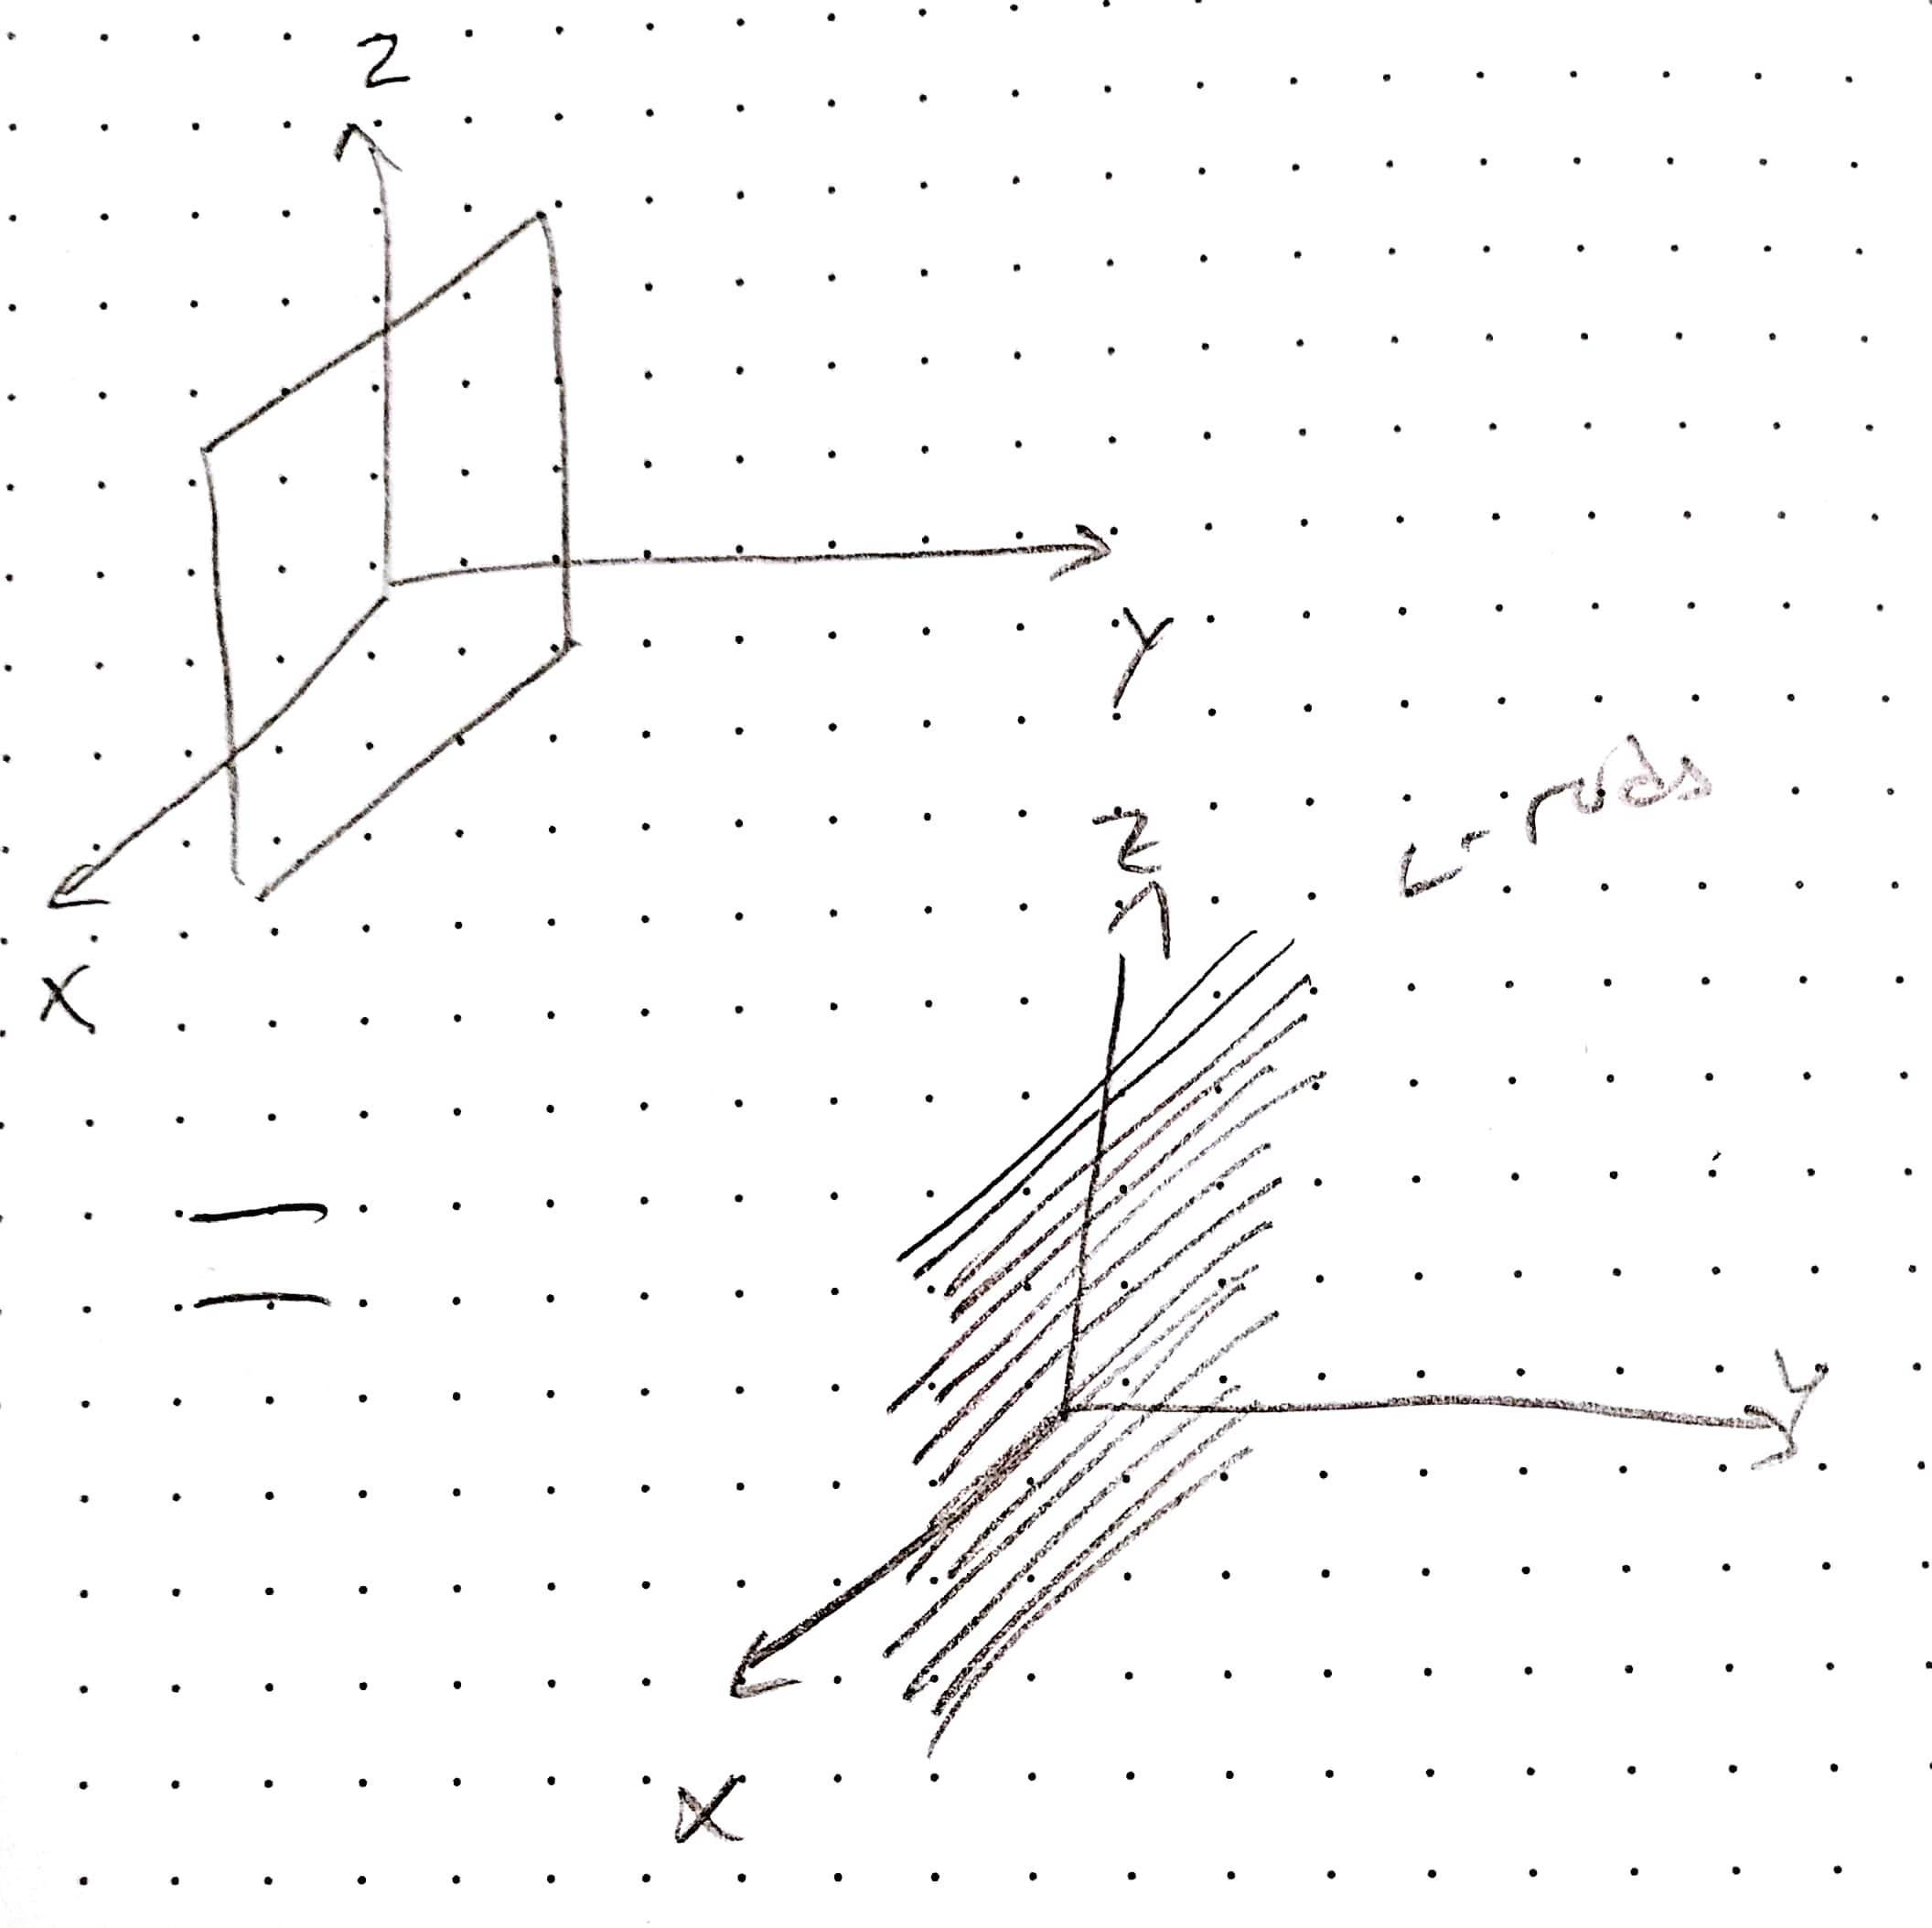
\includegraphics[width=.3\textwidth]{images/Week1pic3.jpg}
\caption{The image is a graphical representation of this method of integrating along an infinite plane. Understand that there are many ways of approaching this problem (i.e. you can integrate along an \textbf{infinite} plane by splitting it into an infinite number of concentric rings.}
\end{figure}\\
\\
Our expression for the electric field due to an infinite rod is $$\vec{E}_{inf rod} = \frac{1}{4\pi\epsilon}\frac{2\rho}{r}\hat{r}$$Recall that $\rho$ is the same as $\frac{\dif q}{\dif A}$. So we still need to integrate along the z direction. We can apply another interesting thing about symmetry. Since the rods are infinite, we can imagine each rod as a point charge having the electric field of the rod, each charge placed along the midpoint. Then, our $r$ is very simple: $r = \sqrt{y^2 + d^2}$, where there is no $x$ dependence. Finally, let us rewrite our expression: $$\vec{E} = \frac{1}{4\pi\epsilon}\int_{-\infty}^{\infty} \frac{2\rho}{\sqrt{y^2 + d^2}}\hat{r} \dif y$$We also know that our $\hat{r} = \frac{\vec{r}}{|\vec{r}|} = \frac{1}{\sqrt{y^2 + d^2}}<d,\ y>$. However, again, because of symmetry, we have that our $y$ components should cancel out since the plane is symmetric along positive and negative $y$ axis. So, we only care about the $z$ component: $\vec{z} = \frac{d}{\sqrt{y^2 + d^2}}\hat{z}$. Let us once again rewrite our integral: $$\vec{E} = \frac{1}{4\pi\epsilon}\int_{-\infty}^{\infty} \frac{2\rho d}{y^2 + d^2} \dif y$$You can then use trigonemtric substitution. As a result of some calculations, the expression condenses to: $$\big|_{-\pi/2}^{\pi/2} 2\rho \theta = \frac{\rho}{2\epsilon}$$
\\
Next, we will discuss a brief introduction to Gauss' Law. A more in depth teaching can be found in the section called "Maxwell's Equations". Here, we will spend more time discussing particular ways of approaching problems. Gauss' Law states that the total electric field flux through a surface is equivalent to the charge enclosed. The simpler equation is as given: $$\oiint_{\dif S} \vec{E} \cdot \hat{n} \dif S= \frac{1}{\epsilon}\sum\limits_i q_i$$To find the charge enclosed, you should understand what this means. If I have a charge density and I construct a surface, you should know that to find the charge enclosed, you should integrate through using the density, since the density represents charge per volume (traditionally). However, for non 3-dimensional problems, you may find these densities to represent charge per area or even charge per length. In addition, you should also understand that when i say $\oiint_{\dif S} \vec{E} \cdot \dif A$, I am saying I want the electric flux through my \textbf{entire} surface (If you want a better understanding of this, refer to the "Maxwell's Equations" section). This integral is very difficult to integrate over. However, looking at this, you may realize that you need to understand how the electric field looks in order to approach this problem. After all, even if you have the charge enclosed, if you don't know how the electric field looks, how can you either evaluate the integral or simplify the integral to solve for the electric field? A prime example can be given by calculating the electric field due to an infinite plate. We know that the electric field should look horizontal everywhere and have the same magnitude along the vertical (it's infinite, after all). So, if we want to find the electric field a distance $x$ from the plate, we should construct a surface that not only encloses charge but also has a constant electric field going through all its faces:
\begin{figure}[ht]
\center
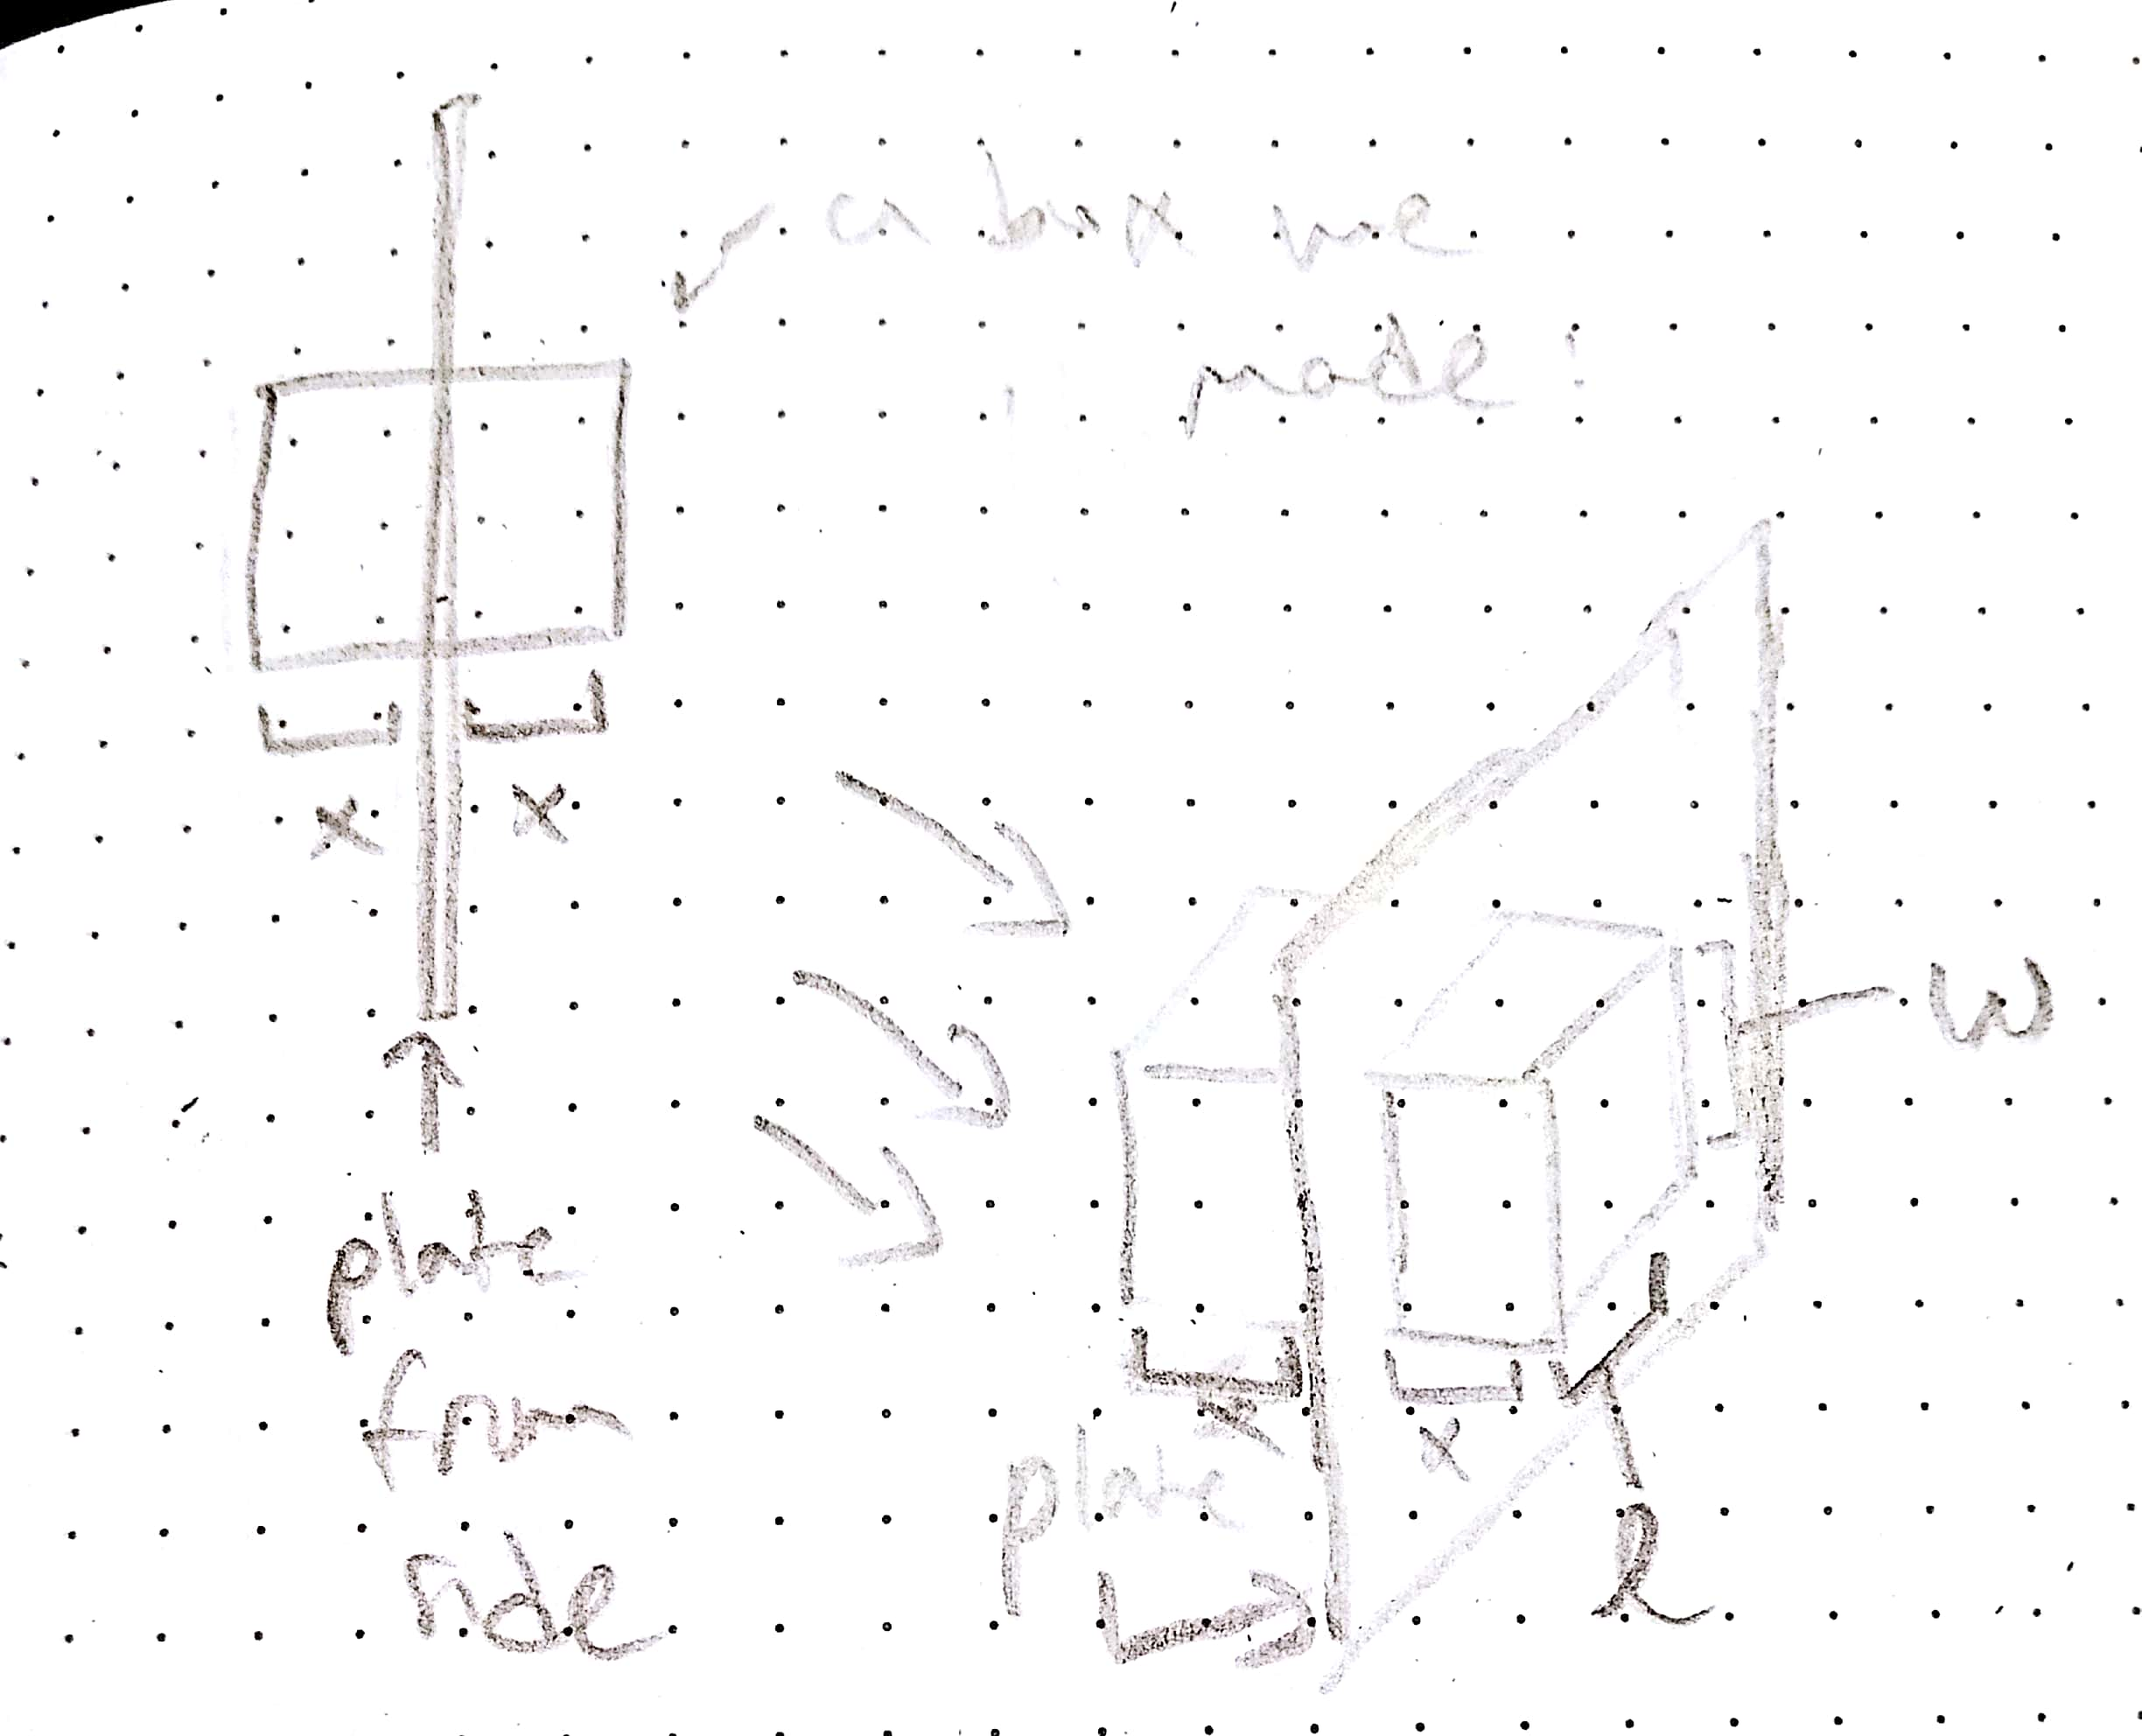
\includegraphics[width=.3\textwidth]{images/Week1pic4.jpg}
\caption{The image is a little blurry, but it represents the box that we constructed around our plate. The box is our surface. As you can see, it stretches out by $x$ on both sides and has a cross-sectional length of $l$ and height of $w$.}
\end{figure}\\
\\
Now we can use Gauss' Law. Let's say our charge density is $\sigma$, as charge per area. Since our plate is infinitely thin, our charge enclosed is from the part of the plate that we are boxing in, which is just $l\times w$. So our charge enclosed is $\sigma * l * w$. So our righthand side is just $$\frac{1}{\epsilon}\sum\limits_i q_i = \frac{\sigma lw}{\epsilon}$$Now our surface is truly useful. Because we know that the electric field should be constant along the vertical since it's infinite, and should also be horizontal everywhere since it's infinite, we can simplify the integral on the left side. So, since the integral on the left is the surface integral, we have to do it for every face of our box. Through every face except the left and right face, we clearly should have no electric field flux. After all, we know the electric field is horizontal everywhere, so the dot product of the horizontal electric field with the perpendicular area vectors of those faces should be $0$ (Remember, area vectors, or $\hat{n} \dif A$) is a vector representing $\dif A$ pointing perpendicular to and out of the surface). So, we are left with having to calculate the electric flux through the left and right faces. But, we know that since the plate is symmetric, it should have the same electric field a distance $x$ from either side, so the electric field should be constant through both faces. Notice also that the electric field going through the left and right faces are perpendicular to those faces, so our equation simplifies: 
\begin{align*}
	\oiint_{\dif S} \vec{E} \cdot \hat{n} \dif A = E*2A.
\end{align*}
You may ask, why does our equation simplify like that? Basically, since our electric field is constant based on our box. So, you can properly see it through this derivation ($S_1$ is left face and $S_2$ is right face. Also there are 6 faces total since we made a box):
\begin{align*}
	\oiint_{\dif S} \vec{E} \cdot \hat{n} \dif A &= \iint_{S_1} \vec{E} \cdot \hat{n} \dif A + \iint_{S_2} \vec{E} \cdot \hat{n} \dif A + \iint_{S_3} \vec{E} \cdot \hat{n} \dif A + \iint_{S_4} \vec{E} \cdot \hat{n} \dif A + \iint_{S_5} \vec{E} \cdot \hat{n} \dif A + \iint_{S_6} \vec{E} \cdot \hat{n} \dif A \\
	&= \iint_{S_1} \vec{E} \cdot \hat{n} \dif A + \iint_{S_2} \vec{E} \cdot \hat{n} \dif A = \iint_{S_1} E \dif A + \iint_{S_2} E \dif A\\
	&= E(\iint_{S_1} \dif A + \iint_{S_2} \dif A)
\end{align*}
$E\cdot \hat{n}$ for $S_1$ and $S_2$ is just $E$ because for the left and right faces, they are pointing in the same direction (electric field points outwards horizontal, and area vectors also point outwards), so the dot product is just as if you multiply their magnitudes. In addition, as I said before, the electric field is constant here so we can just pull it out. The expression: $\iint_{S_1} \dif A$ is the same as asking for the area of that face. Continuing on, we should now finalize our calculations.
We know that our area of those two faces is simply $A = lw$. Thus, our expression condenses to:
\begin{align*}
	E*2lw = \frac{\sigma lw}{\epsilon}
\end{align*}
Notice that we have beautifully simplified our originally complex looking Gauss' Law to a simple equation. Now, we can solve the the electric field at a distance $x$ from it (We don't define x because we want to calculate the electric field for any arbitrary x from the plate). So, our final expression for electric field is:
\begin{align*}
	E =  \frac{\sigma}{2\epsilon}
\end{align*}
Notice how it is the same as the way we calculated it earlier by performing the very convoluted integral $$\vec{E} = \frac{1}{4\pi\epsilon}\int_{-\infty}^{\infty} \frac{2\rho d}{y^2 + d^2} dy$$
\\
\\
\\
Now, for the final section of week 1, I will discuss the idea behind conductors. The basic idea of a conductor is that a material that is a conductor will have electrons that are free to move. In addition, know that every metal is a conductor. So, what does it mean for electrons to be able to move freely? This means that if I apply an electric field on those electrons, they will move, creating a charge distribution that will cancel out the electric field. But, why does it cancel? Think of it like this: If I have an electric field, surely my electrons will move. But, by moving, the net charge must remain constant, so there will be some positive charge on the opposite end. If my electric field is 0, I wont accelerate.:
\pagebreak
\begin{figure}[ht]
\center
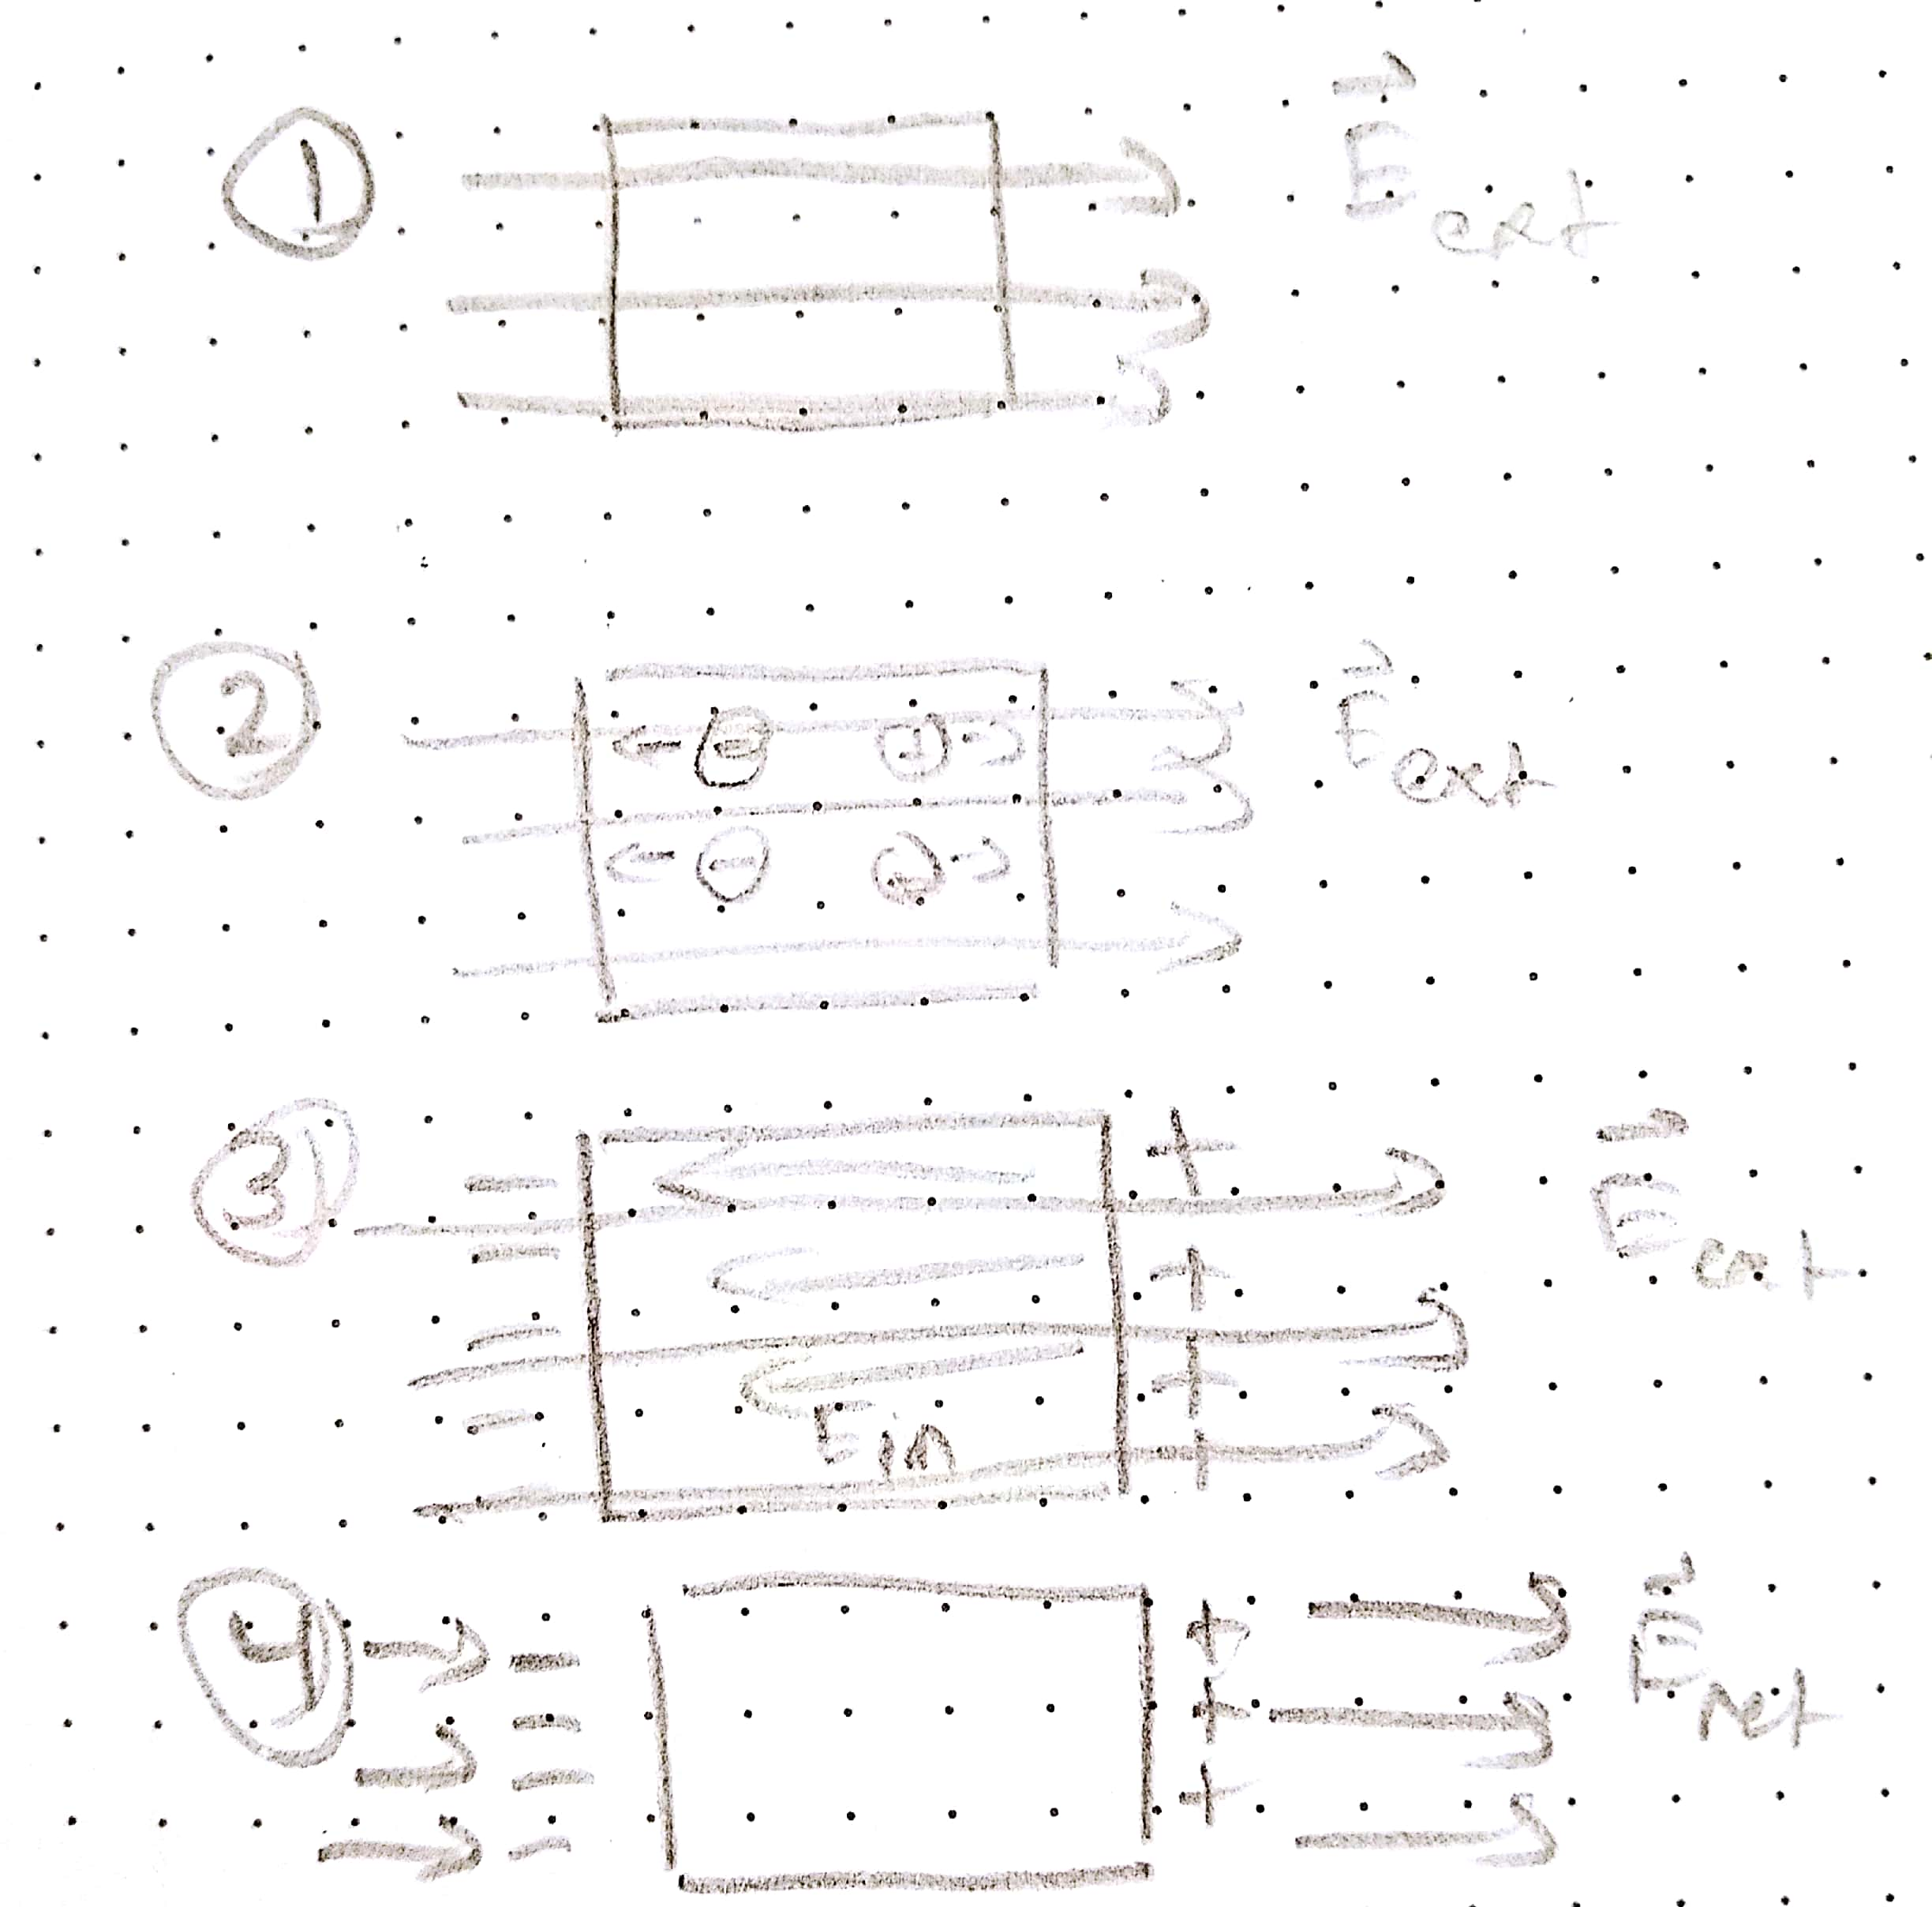
\includegraphics[width=.3\textwidth]{images/Week1pic5.jpg}
\caption{This image demonstrates the general process by which a metal maintains a 0 net electric field inside. The charges move and build up a net charge along the surface that opposes the external field}
\end{figure}

Note that the movement of the charge creates a charge distribution on the surface of the metal. Note that this is the net representation. In reality, I still have negative and positive charges in the metal itself. However, they all cancel, so the net effect is as if I only have charge on the surface. This charge build up will keep building up as long as my net electric field inside is non-zero, so it will eventually cancel out. Note, the charge on either side must be the same because the net charge should still be $0$ (since my metal was neutrally charged to begin with). This also means that if I had a net charge $Q$, the sum of my surface charges must have the net charge $Q$. After all, my charges have only moved. I haven't added or taken away any charge by applying my external electric field. 
\\
\\
\textit{Interesting result: If you want to think of energy, you may wonder: If my external field is gone, didn't I lose energy? That energy has been distributed along the outside. If you look at the distribution, you may notice that it is like a dipole, where the electric field outside of the metal due to this distribution is the same direction as the external field. As a result, we have a stronger electric field outside.}
\\
\\
Speaking of energy, that leads to the next section: Week 2.
\pagebreak

\section{Week 2}
I will now begin to talk about energy and electric potential (voltage). There is a very special feature of coulomb force and gravitational fields. That is, they are conservative forces. When I say conservative, I mean that if I were to change my position, I can always return that energy by reversing the process. Aka, if I move from point A to point B, then from point B to point A, I should have a $0$ net change in energy. In addition, all Coulomb electric fields (fields due to charges) are conservative. This not only means what we mentioned earlier with point A and point B, but also that no matter what path I take from point A to point B, I will have the same change in energy. With electric fields, we define the electric potential, or energy per charge, as the voltage. This is defined by: $$V = -\int_A^B \vec{E} \cdot \dif \vec{s}$$The equation represents the idea that along my path, I take the dot product of the electric field and the direction I am moving (essentially says I want to multiply the part of my field along my path by the direction). Notice its similarity to the definition of energy: $E = \int \vec{F} \cdot \dif \vec{s}$. Cumulatively, with the idea of conservative fields, this means that for coulomb fields, we should have $$-\oint \vec{E} \cdot \dif s = \oint \vec{E} \cdot \dif s = 0$$This is true, because the loop integral says I make a full loop, or I end at where I started. By the idea of conservative fields, if I return to the same location, I should have a $0$ change in energy. It is essential to realize that electric potential only carries meaning when you describe its potential in its difference with respect to its potential at another point. This is why we define it with the integral. \\
\\
Now, another important concept is the idea of reference points. When I say reference point, I say: what is my potential with respect to that point. This is also equivalent to treating that reference point as having 0 potential. You may question: But if I use the equation and do $\int_A^B \vec{E} \cdot \dif \vec{s}$, clearly I will end up with $V(B) - V(A)$, and $V(A)$ may not necessarily be 0. However, if I say my refernce point is $A$, the equation can be looked at in this form: $$(V(B)-V(A)) - 0$$If you notice, with this representation, it is saying, if I take my voltage at $A$ to be 0, what is my voltage at $B$? It must be the voltage with respect to, hence $V(B)- V(A)$. Another important point about reference points. Choose your reference points wisely. After all, for any problem, you should define your reference point and do all calculations with the same reference point. For many problems, you will likely use $r = \infty$ as a reference point. This is because it not only evaluates to the physical value $0$ but also because it is continuous through it (as opposed to evaluating the potential at $r = 0$).\\
\\
So, how can we approach an actual problem by understanding this? Let us supposed we have a configuration: 

\pagebreak
\begin{figure}[ht]
\center
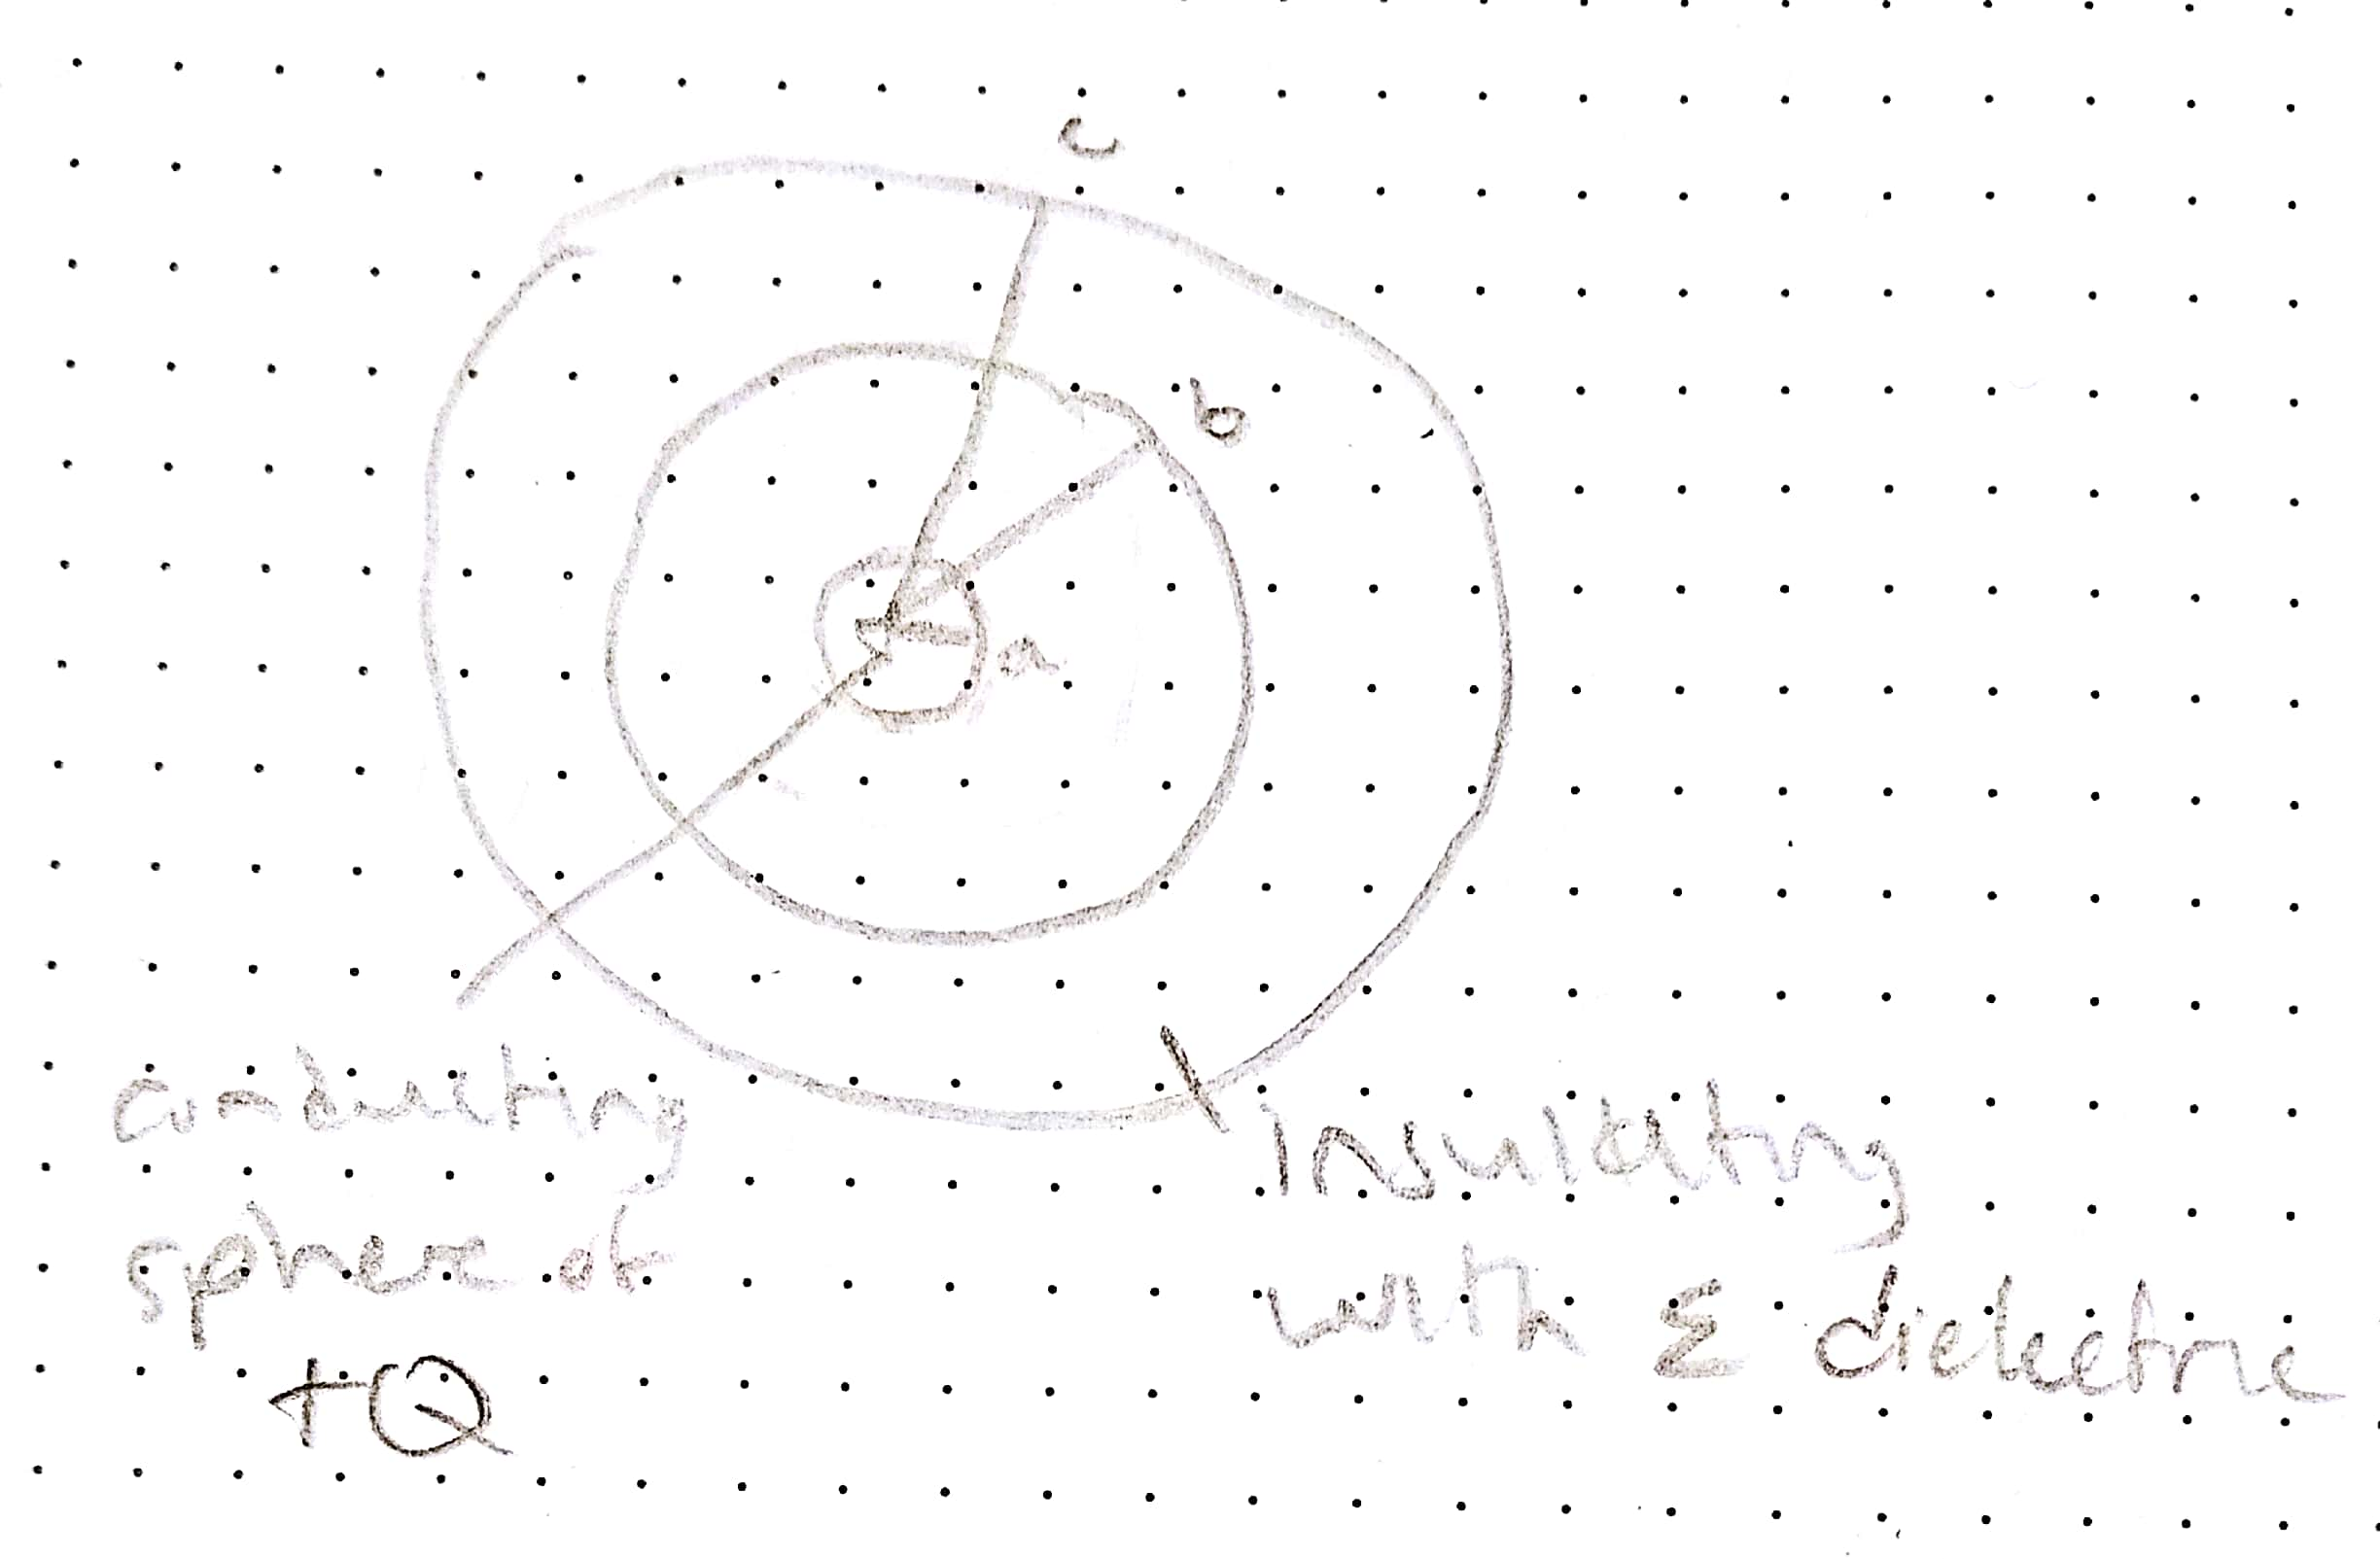
\includegraphics[width=.3\textwidth]{images/Week2pic1.jpg}
\caption{The image represents a conducting sphere in the center, surrounded by an insulating shell with a dielectric constant $\epsilon$. We'll call this $\epsilon_r$. The radius to useful points are given.}
\end{figure}

So, the problem is that I want to evaluate the electric potential at any point. What does this mean? It means that I have to evaluate the electric potential anywhere in space with respect to some reference point. It would be best to use $\infty$ as my reference point here, since the evaluation of an electric potential (as in take the indefinite integral of the electric field with respect to $r$. This is just saying what is the mathematical calculated value, since electric potential is supposed to be with respect to some point) at $\infty$ is conveniently 0. Thus, we must start from infinity and move closer. We can understand that every point in space is some radial distance from the center. In addition, due to symmetry, we can say that any point along the same radius should have the same electric potential. Thus, we can make our path from $\infty$ easier by moving along one of the radiuses. This is because it makes the dot product much more convenient, since the direction vector and electric field vector are parallel. Another important thing to realize is that our electric field at different radii is different. In the conducting sphere, we have $0$, but between $a$ and $b$, we have some electric field, and in the shell, we have another electric field (different due to it being a dielectric). I will speak briefly about the general concept of dielectrics:\\
\\
\subsection{Dielectrics}
A dielectric material is, in general, an insulating material. This can apply to almost any material, whether it be a solid, liquid, or gas. Unlike metals, which have free-electrons, there is less freedom in dielectrics. When you apply an electric field on a dielectric, we still have electric field inside the dielectric. However, the field would weaken within, since, like metals, dielectrics still polarize, just less. You can think of every atom in the material as having orbiting electrons. These electrons, in response to the external field, will align to favor one side. In addition, this leaves the positive charges on the other side, creating a mini-dipole. This can be visually simplified to the idea below:
\begin{figure}[ht]
\center
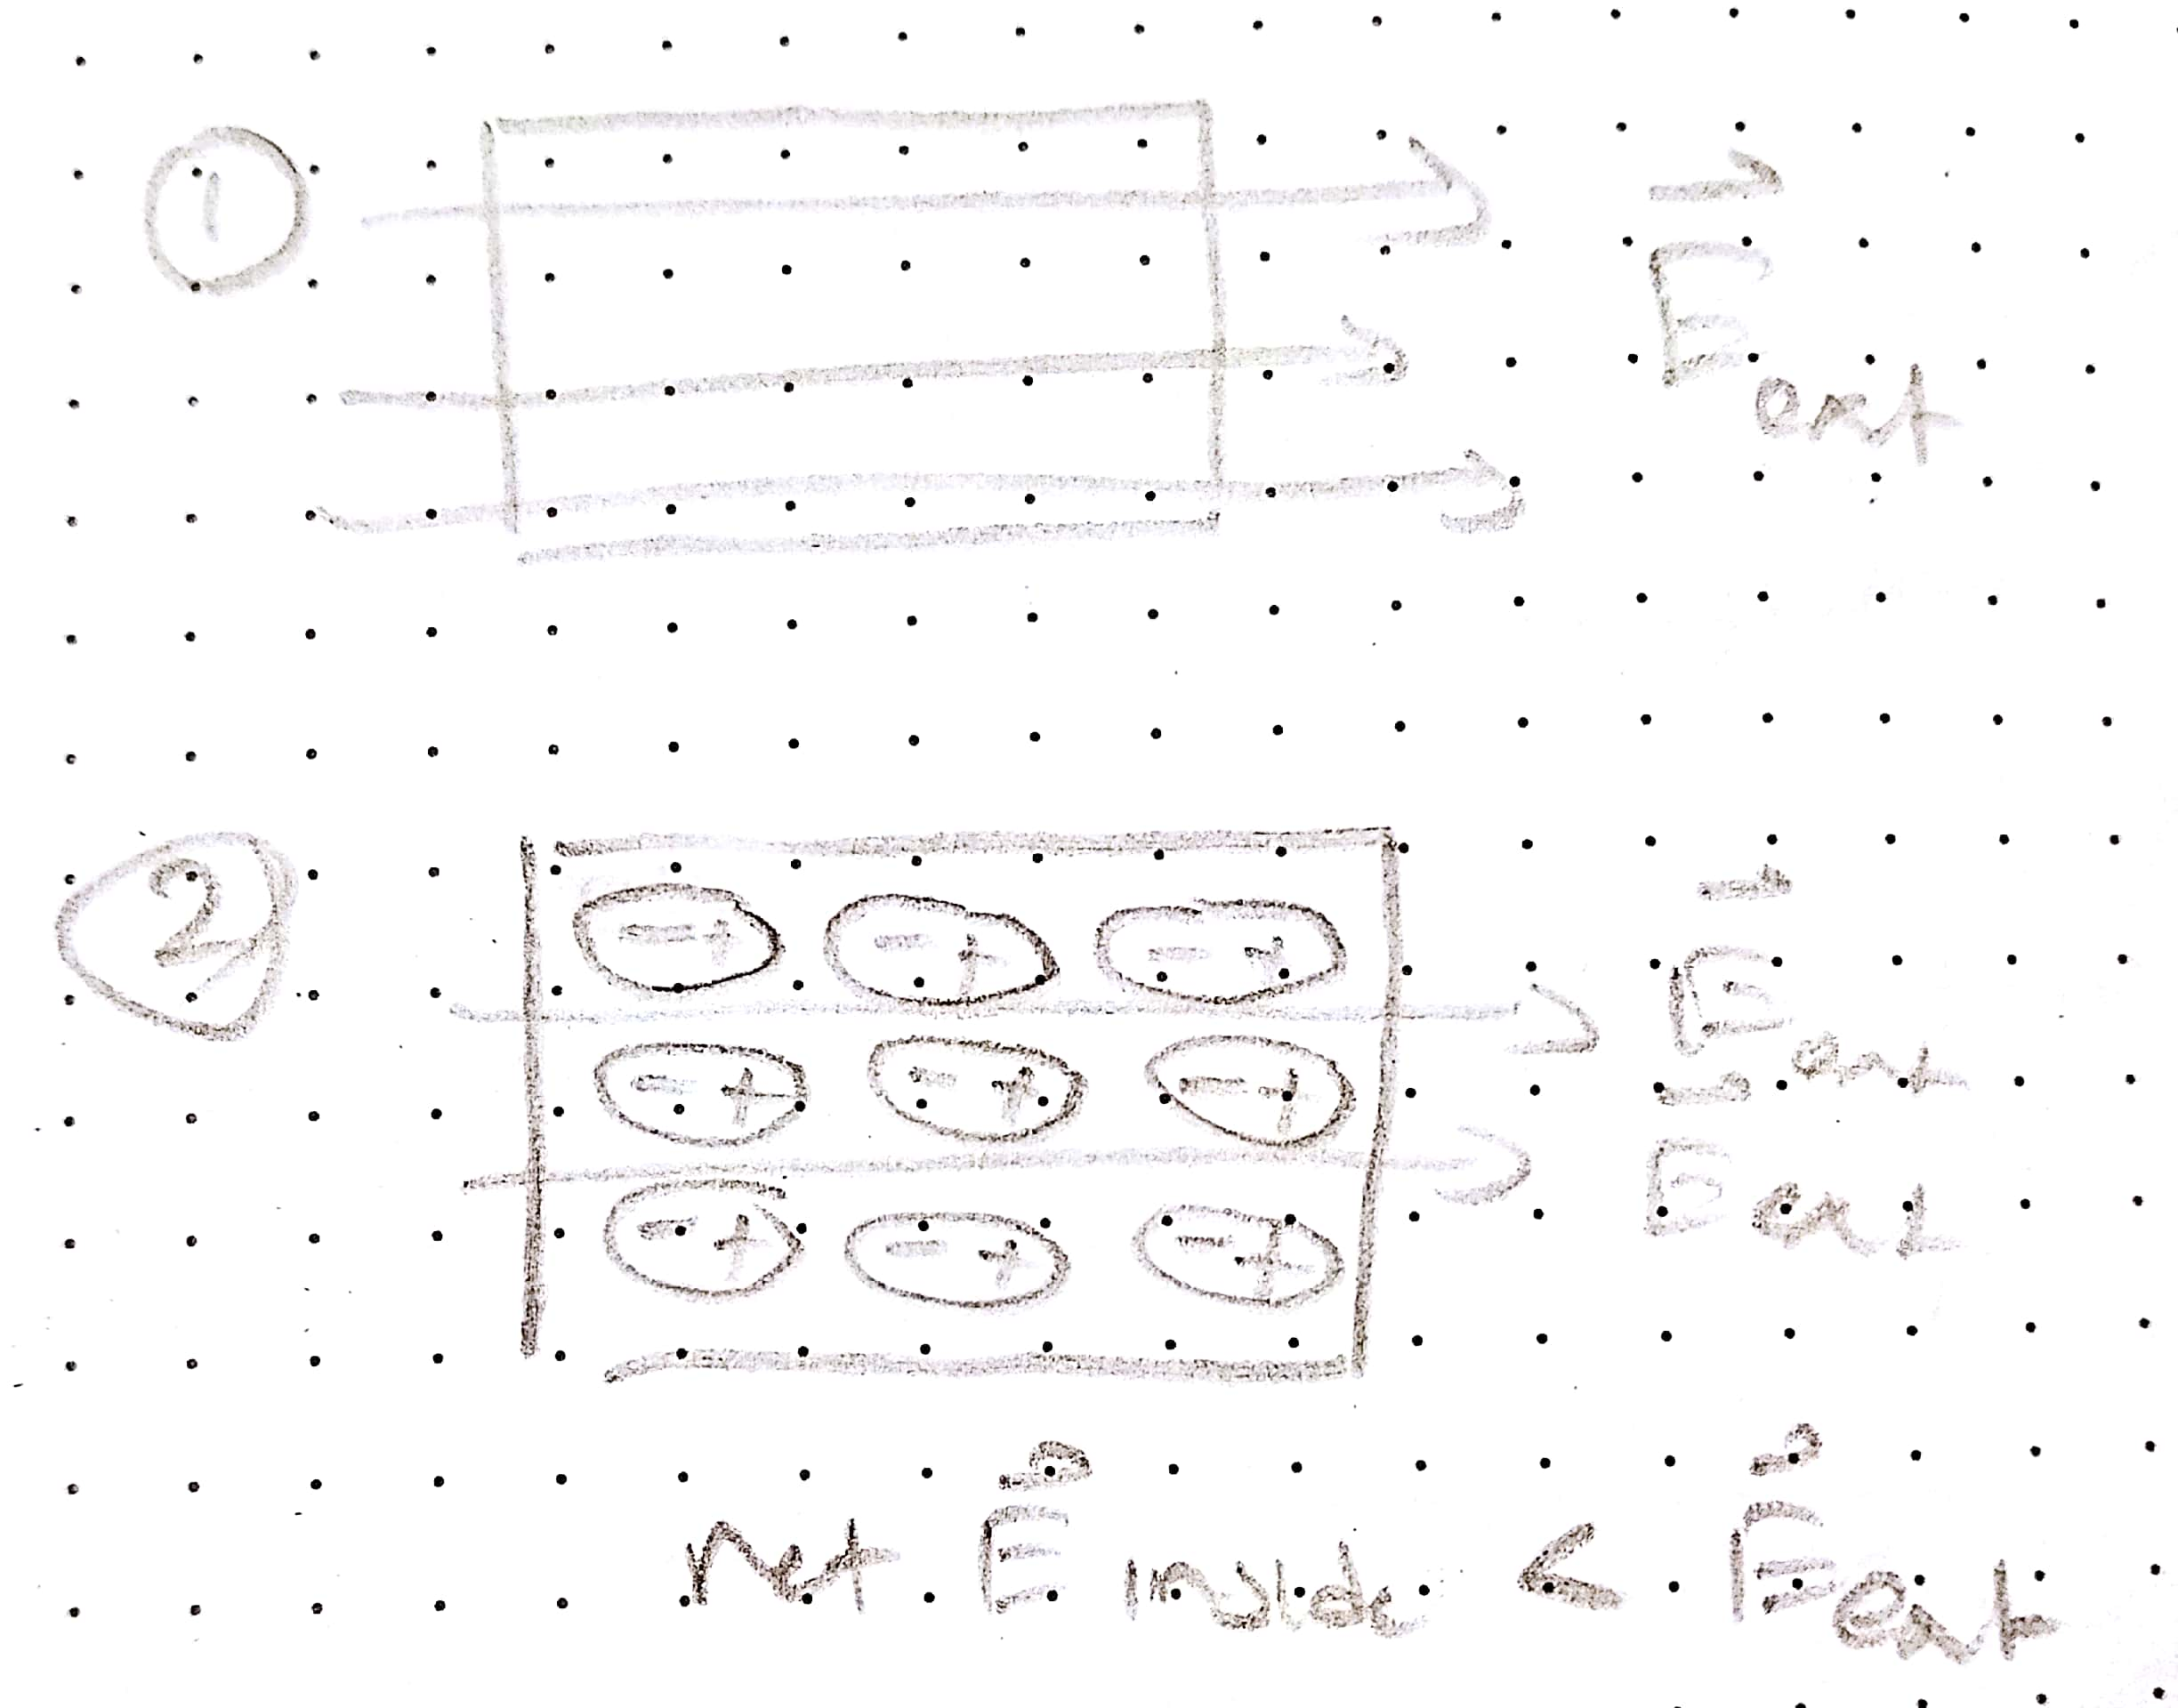
\includegraphics[width=.3\textwidth]{images/Week2pic2.jpg}
\caption{The image displays the effect of an electric field on a dielectric. Notice how internals dipoles form. These produce a net electric field in the opposite direction.}
\end{figure}
\\
Back to the problem at hand, if we wish to calculate the electric potential at any point in space, we need to separate our integral depending on what point we are going to. Thus, we have 4 cases:
\begin{align*}
r > c\\
b < r < c\\
a < r < b\\
r < a
\end{align*}
To begin, we must understand that our reference point is $\infty$, so we must always begin there. For $r > c$, we have a vacuum. In addition, due to the sphere of charge in the center, we have the electric field due to a point charge in a vacuum: $\vec{E} = \frac{1}{4\pi\epsilon_0}\frac{Q}{|r|^2}\hat{r}$. So, the potential outside is given by $$V = -\int_\infty^r \vec{E} \cdot \dif \vec{s}$$Since we are moving along the radial direction, we have:
\begin{align*}
V &= -\int_\infty^r \vec{E} \cdot \dif \vec{r}\\
V &= -\int_\infty^r E \dif r
\end{align*}
Then, let us evaluate:
\begin{align*}
V &= -\frac{1}{4\pi\epsilon_0}\int_\infty^r \frac{Q}{r^2}\dif r\\
V &= \frac{1}{4\pi\epsilon_0}\left(\frac{Q}{r} \bigg|_\infty^r\right) = \frac{1}{4\pi\epsilon_0}\left(\frac{Q}{r} - \frac{Q}{\infty}\right) = \frac{1}{4\pi\epsilon_0}\left(\frac{Q}{r}-0\right)\\
V &= \frac{1}{4\pi\epsilon_0}\frac{Q}{r}
\end{align*}
For the next phase, we need to evaluate the potential in the shell. Notice that we should always start with the same form:$$V = -\int_\infty^r \vec{E} \cdot \dif \vec{s}$$However, our electric field is partitioned, so we have the derived expression:
\begin{align*}
V &= -\int_\infty^r \vec{E} \cdot \dif \vec{s}\\
V &= -\left(\int_\infty^c \frac{Q}{4\pi\epsilon_0 r^2} \dif r + \int_c^r \frac{Q}{4\pi\epsilon_0\epsilon_r r^2} \dif r\right)\\
V &= -\frac{1}{4\pi\epsilon_0}\left(\int_\infty^c \frac{Q}{r^2}\dif r + \frac{1}{\epsilon_r} \int_c^r \frac{Q}{r^2} \dif r \right)
\end{align*}
In addition, we notice that we have already evaluated the expression for one of the expressions in step 1. So, our condensed form is:$$V = \frac{1}{4\pi\epsilon}\frac{Q}{c} + \left(-\frac{1}{4\pi\epsilon_0\epsilon_r} \int_c^r \frac{Q}{r^2} \dif r\right)$$
Why does our form contain the previous voltage? This is simply a result of understanding conservative fields. We define our potential by $V = -\int \vec{E} \cdot \dif \vec{s}$. However, notice that since our field is conservative, the path we take does not matter. Because we are following the same path, however, we must go through the point $c$, which is contained in how we evaluated for the potential outside of the shell. As a result of the field being conservative and how we go through point $c$, our total energy is an arithmetic sum of the potential to point $c$ and the potential from $c$ to $r$. And again, we can go any path, so it's very possible that this integral could have been separated numerous times by different points. However, that would only be redundant. In addition, there would still be the difference in electric field between $b<r<c$ and $r > c$, so we would always have to go through the radius $c$ to get inside. And finally, our field is radial, so we have to pass through point $c$, since $c$ is a radius, not a physical point in space. For the purpose of the problem, we proceed to calculate:
\begin{align*}
V &= \frac{1}{4\pi\epsilon}\frac{Q}{c} - \frac{1}{4\pi\epsilon_0\epsilon_r} \int_c^r \frac{Q}{r^2} \dif r\\
V &= \frac{1}{4\pi\epsilon}\frac{Q}{c} + \frac{1}{4\pi\epsilon_0\epsilon_r}\left(\frac{Q}{r}-\frac{Q}{c}\right)
\end{align*} 
Proceeding, we now include the partition of $a < r < b$, which is in a vacuum. So, using the previous form, our calculation follows:
\begin{align*}
V &= \frac{1}{4\pi\epsilon}\frac{Q}{c} + \frac{1}{4\pi\epsilon_0\epsilon_r}\left(\frac{Q}{b}-\frac{Q}{c}\right) - \frac{1}{4\pi\epsilon_0}\int_b^r \frac{Q}{r^2}\dif r\\
V &= \frac{1}{4\pi\epsilon}\frac{Q}{c} + \frac{1}{4\pi\epsilon_0\epsilon_r}\left(\frac{Q}{b}-\frac{Q}{c}\right) + \frac{1}{4\pi\epsilon_0}\left(\frac{Q}{r}-\frac{Q}{b}\right)
\end{align*}
Finally, we know that in a conducting sphere, we have no electric field inside, so the expression for potential inside the sphere should be constant anywhere inside:
$$V = \frac{1}{4\pi\epsilon}\frac{Q}{c} + \frac{1}{4\pi\epsilon_0\epsilon_r}\left(\frac{Q}{b}-\frac{Q}{c}\right) + \frac{1}{4\pi\epsilon_0}\left(\frac{Q}{a}-\frac{Q}{b}\right)$$
A side note: One may think that the form $V = -\int \vec{E} \cdot \dif \vec{r}$ for this problem should yield $V = \int E \dif r$ because you are moving opposite the direction of the field. However, when doing line integrals, you either fix the path, or fix the limits. In this case, we are fixing the path. This is why we choose $\dif \vec{r}$. The direction of $\vec{r}$ is always pointing radially outwards from the source. Thus, our dot product should not change the sign. However, our limits go from the further radius to the smaller radius. \\
\\
Now, this next section will cover circuits. Be aware, this section does not go too in depth on the equations such as the total capacitance or total resistance, but more covers loop rule and other important concepts in circuitry. There are several key concepts to understand before delving into circuitry. One important concept is drift velocity. In any current carrying wire, there are electrons moving, but they are moving in different directions. However, because of the electric field, they must all have a horizontal component in the same direction. We can quantize this average velocity as the drift velocity. There is another constant called mobility, or the average drift velocity per electric field (strength). Meaning, for a given electric field through a portion of the wire, we can calculate the average drift velocity with this measured constant: $$\vec{\nu} = \vec{E}\nu$$Where $\nu$ is the drift velocity and $\nu$ is the mobility constant. From here, there is another important quantity to measure: Charge per second, or an current ($I$). This is an important quantity because it is very useful for measurement and many other calculations surrounding circuits. When we say charge per second, we mean that let me choose some point along the wire. I want to know, per second, how many Coulombs pass through that point. An interesting way to calculate this given the drift velocity is the choose some point. Let me choose 1 charge at that point and have it move at the drift velocity for $1$ second. After $1$ second, it'll clearly end up at another point. Clearly, at the second point, it has not gone beyond that point. However, at the same time, it clearly passed all the points between the initial and final point. This is also the same thing as saying all the charge between those two points (initially) have definitely passed through the final point, since the other charges were ahead of this charge we chose. So, it's as if all the charges enclosed in this volume between the initial and final point have passed through the final point after $1$ second. So, if I can find how much charge was enclosed in that volume, then I know how much charge passes a point per second with the average drift velocity. 
\pagebreak
\begin{figure}[ht]
\center
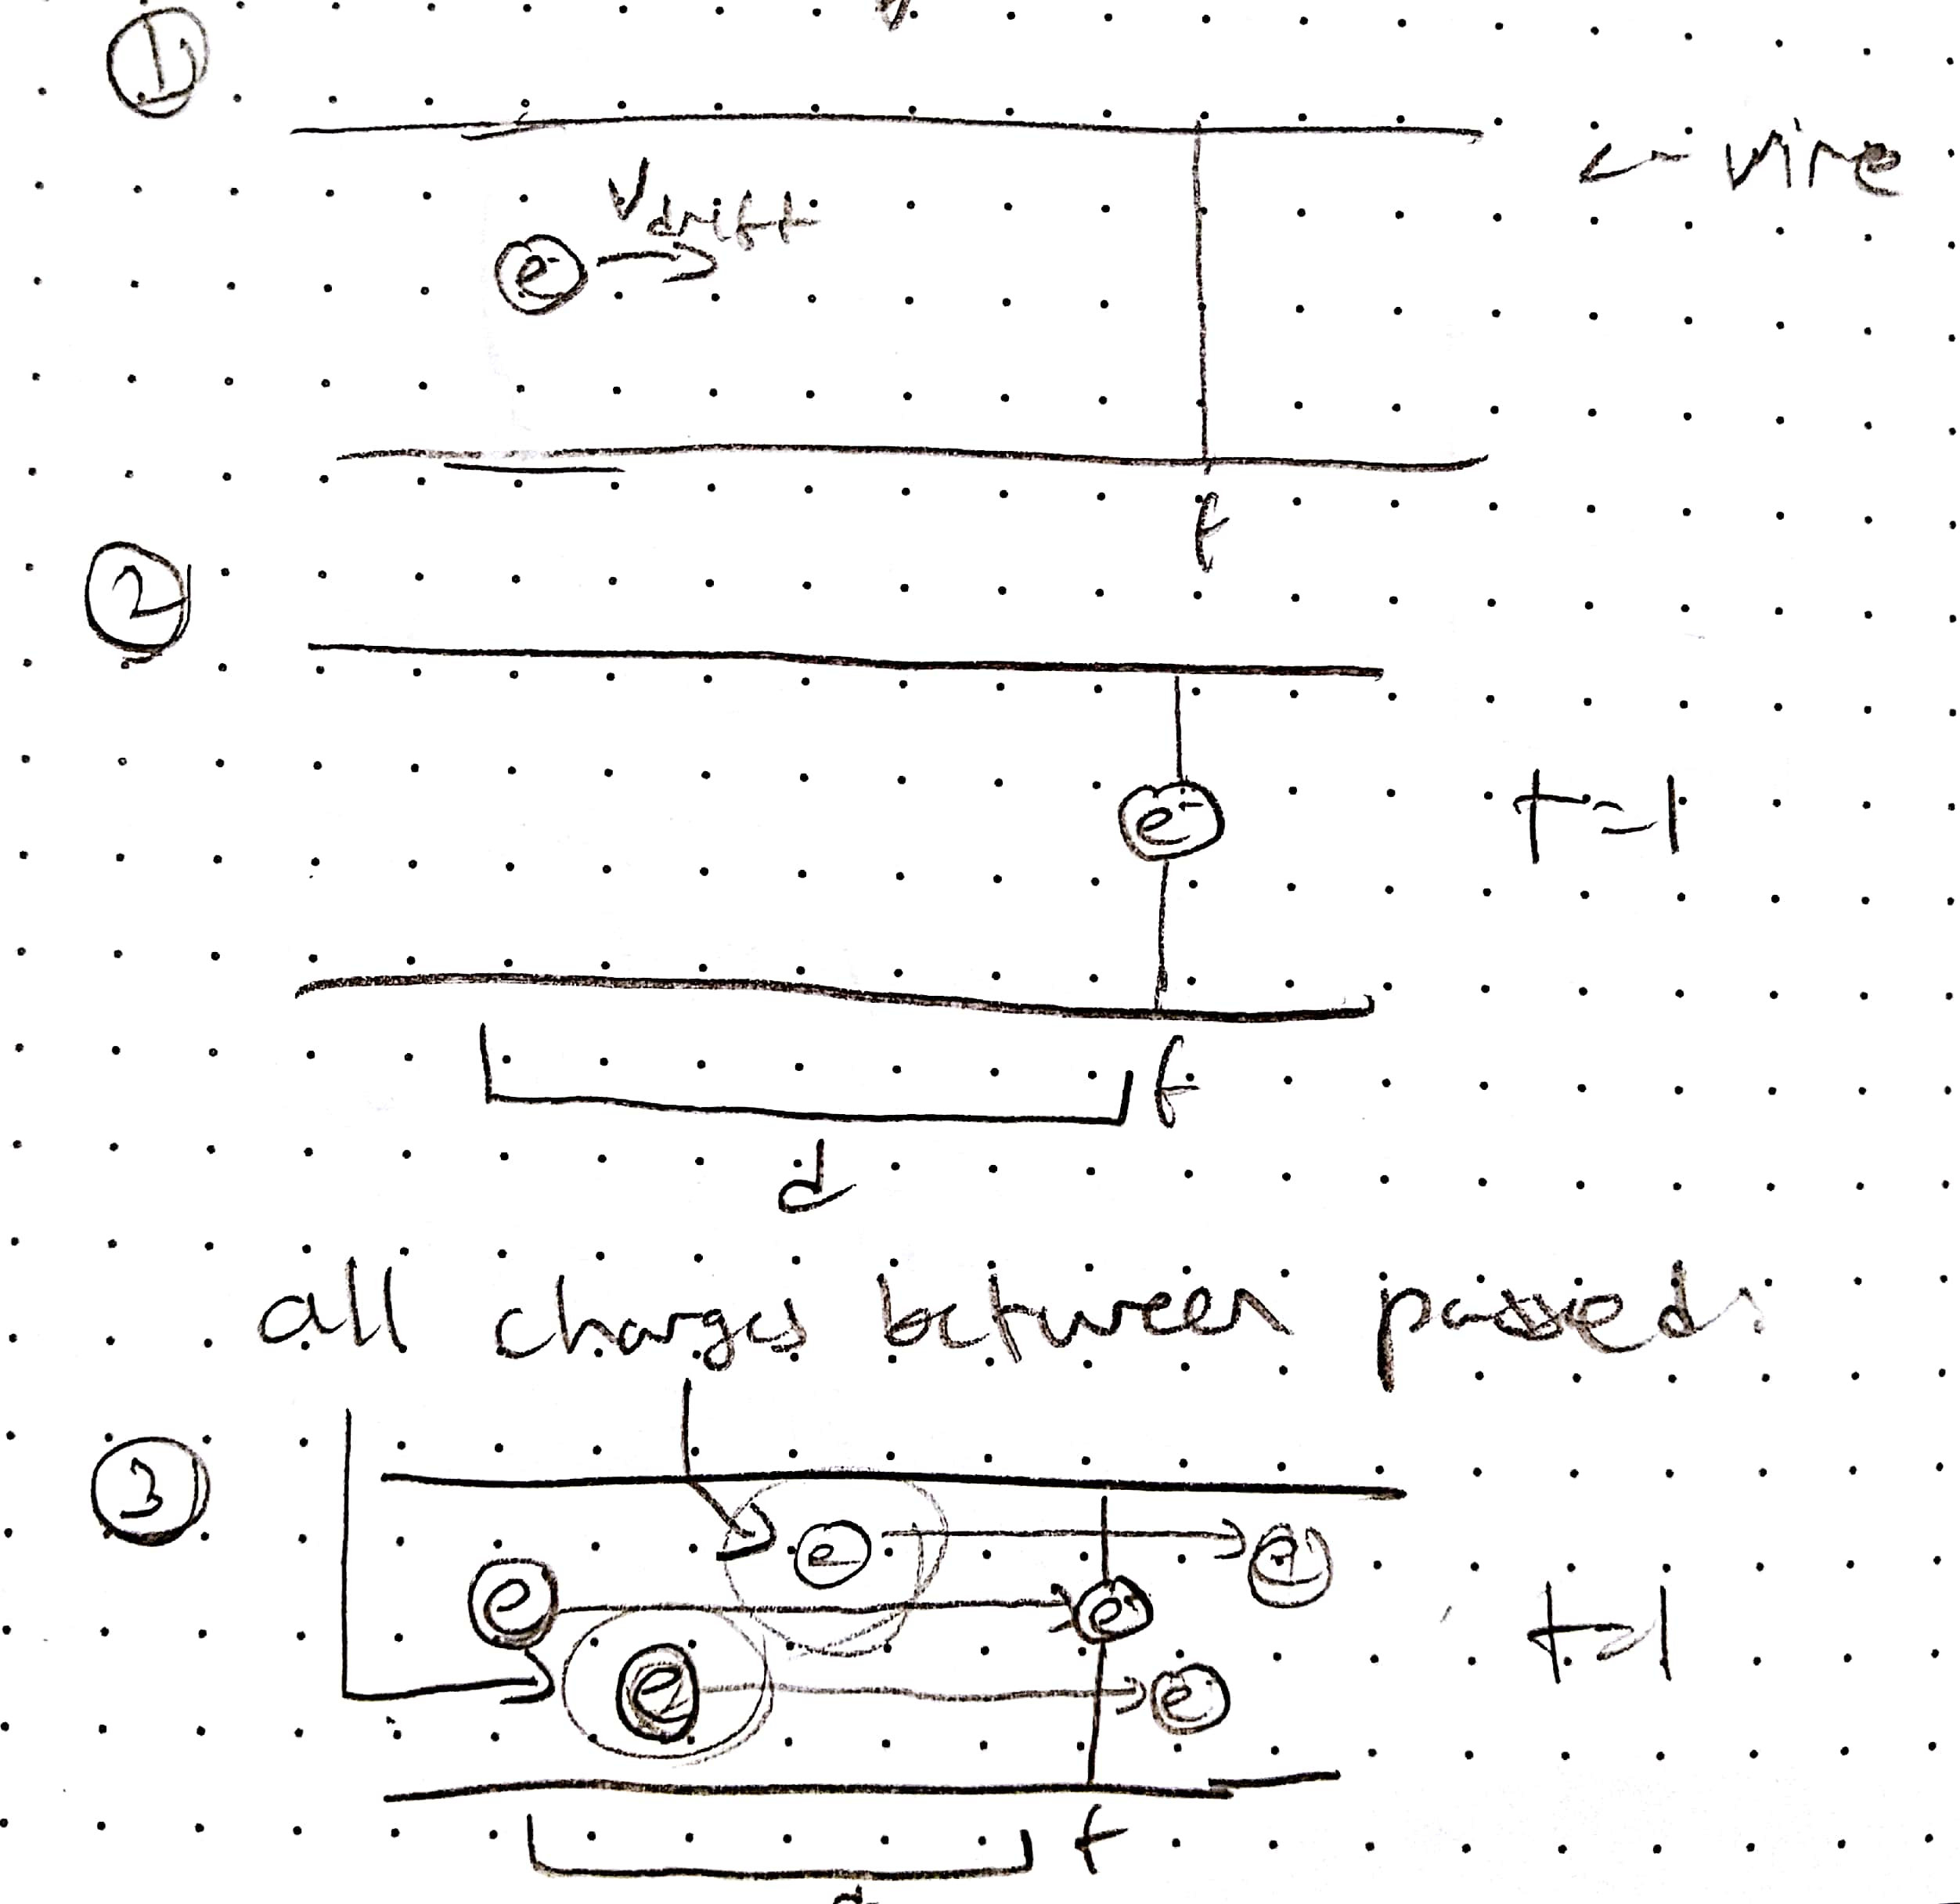
\includegraphics[width=.3\textwidth]{images/Week2pic3.jpg}
\caption{The image shows what I mean by all the charge enclosed in the volume after 1 second should have also passed the point the charge you chose ended up at: point $f$}
\end{figure}
\\
So, the calculation should follow:
\begin{align*}
I &= \frac{Q}{t}\\
&= \frac{\rho V}{t}\\
&= \frac{\rho lA}{t}\\
&= \frac{\rho \nu t A}{t}\\
&= \frac{\rho |\vec{E}|\nu t A}{t}\\
&= \rho |\vec{E}|\nu A
\end{align*}
Usually, you will know the number of charge carriers per volume rather than Coulombs, so instead of $\rho$, you will have $n$, so the expression must be multiplied by the charge in Coulombs per charge carrier (usually same magnitude as electron): $$I = n|\vec{E}|\nu Ae$$If you know the drift velocity, then: $I = nA\nu e$. 
Now that we understand how we can calculate current by an electric field, we have understood, at the microscopic level, how electric fields move charges, and how we call something "current". The next step is understanding, briefly, how batteries provide a constant voltage across an entire circuit. In voltaic cells, or batteries that we will focus on, they undergo a chemical process called oxidation and reduction reactions. Generally, by the chemical process, charge is produced and a voltage difference is generated. After all, a potential difference is energy, so to keep that constant while it is constantly being used, you need a constant chemical energy process. This is also why batteries eventually deteriorate. Batteries are unique in that they store the electrical energy via chemical energy. There is another way of storing energy. However, unlike batteries, it is not chemical and it does not constantly output the same voltage. These are called capacitors. Capacitors are unique for a couple of reasons. If a charged capacitor is placed in a circuit, it'll act like a battery, except the charge on the plates will disperse (there is no constant supply of charge), so you can expect the current to drop over time. Now, I will discuss a common form of a capacitor: two parallel plates. These parallel plates are responsible for accumulating the charge in the circuit. Now, from the previous understanding of electric fields, there is an electric field due to these plates. In addition, these plates then to be large compared to the small distance between, leading it to be similar to the parallel infinite plate setup, with an electric field of:$$\vec{E} = \frac{\sigma}{\epsilon}$$Now there is another important thing to realize. That is, with an electric field beteen these plates, there is clearly a potential difference as well. That would be: $$\Delta V = \int_0^d \frac{\sigma}{\epsilon} \dif r$$The reason why we don't care about the sign in front of the integral is because we're just showing the difference in potential. If you would like to be more formal with directions, it would be negative in the form we constructed because I am moving from $0$ (what I choose to be my reference point) to $d$. The electric field, being positive, means that I am moving along it. So, my potential surely would decrease and be kinetic energy instead. But, as I said, what is of importance is understanding what it means to have a potential difference across these plates. \\
\\
\subsection{Energy Density}
Another important concept when understanding the energy stored by electric fields is by understanding energy density. Simply put, we say energy density is the energy per unit volume. But, how can we understand what it means to have an energy density? Well, we can imagine this as having two infinitely large parallel charged plates. So, basically, I want to see how my energy changes as I increase the space between the two, or the volume, or energy per volume. Basically, I will move some arbitrary group of charge parallel to the other plate from the reference point to some other point and divide it by the volume enclosed. 

\begin{figure}[ht]
\center
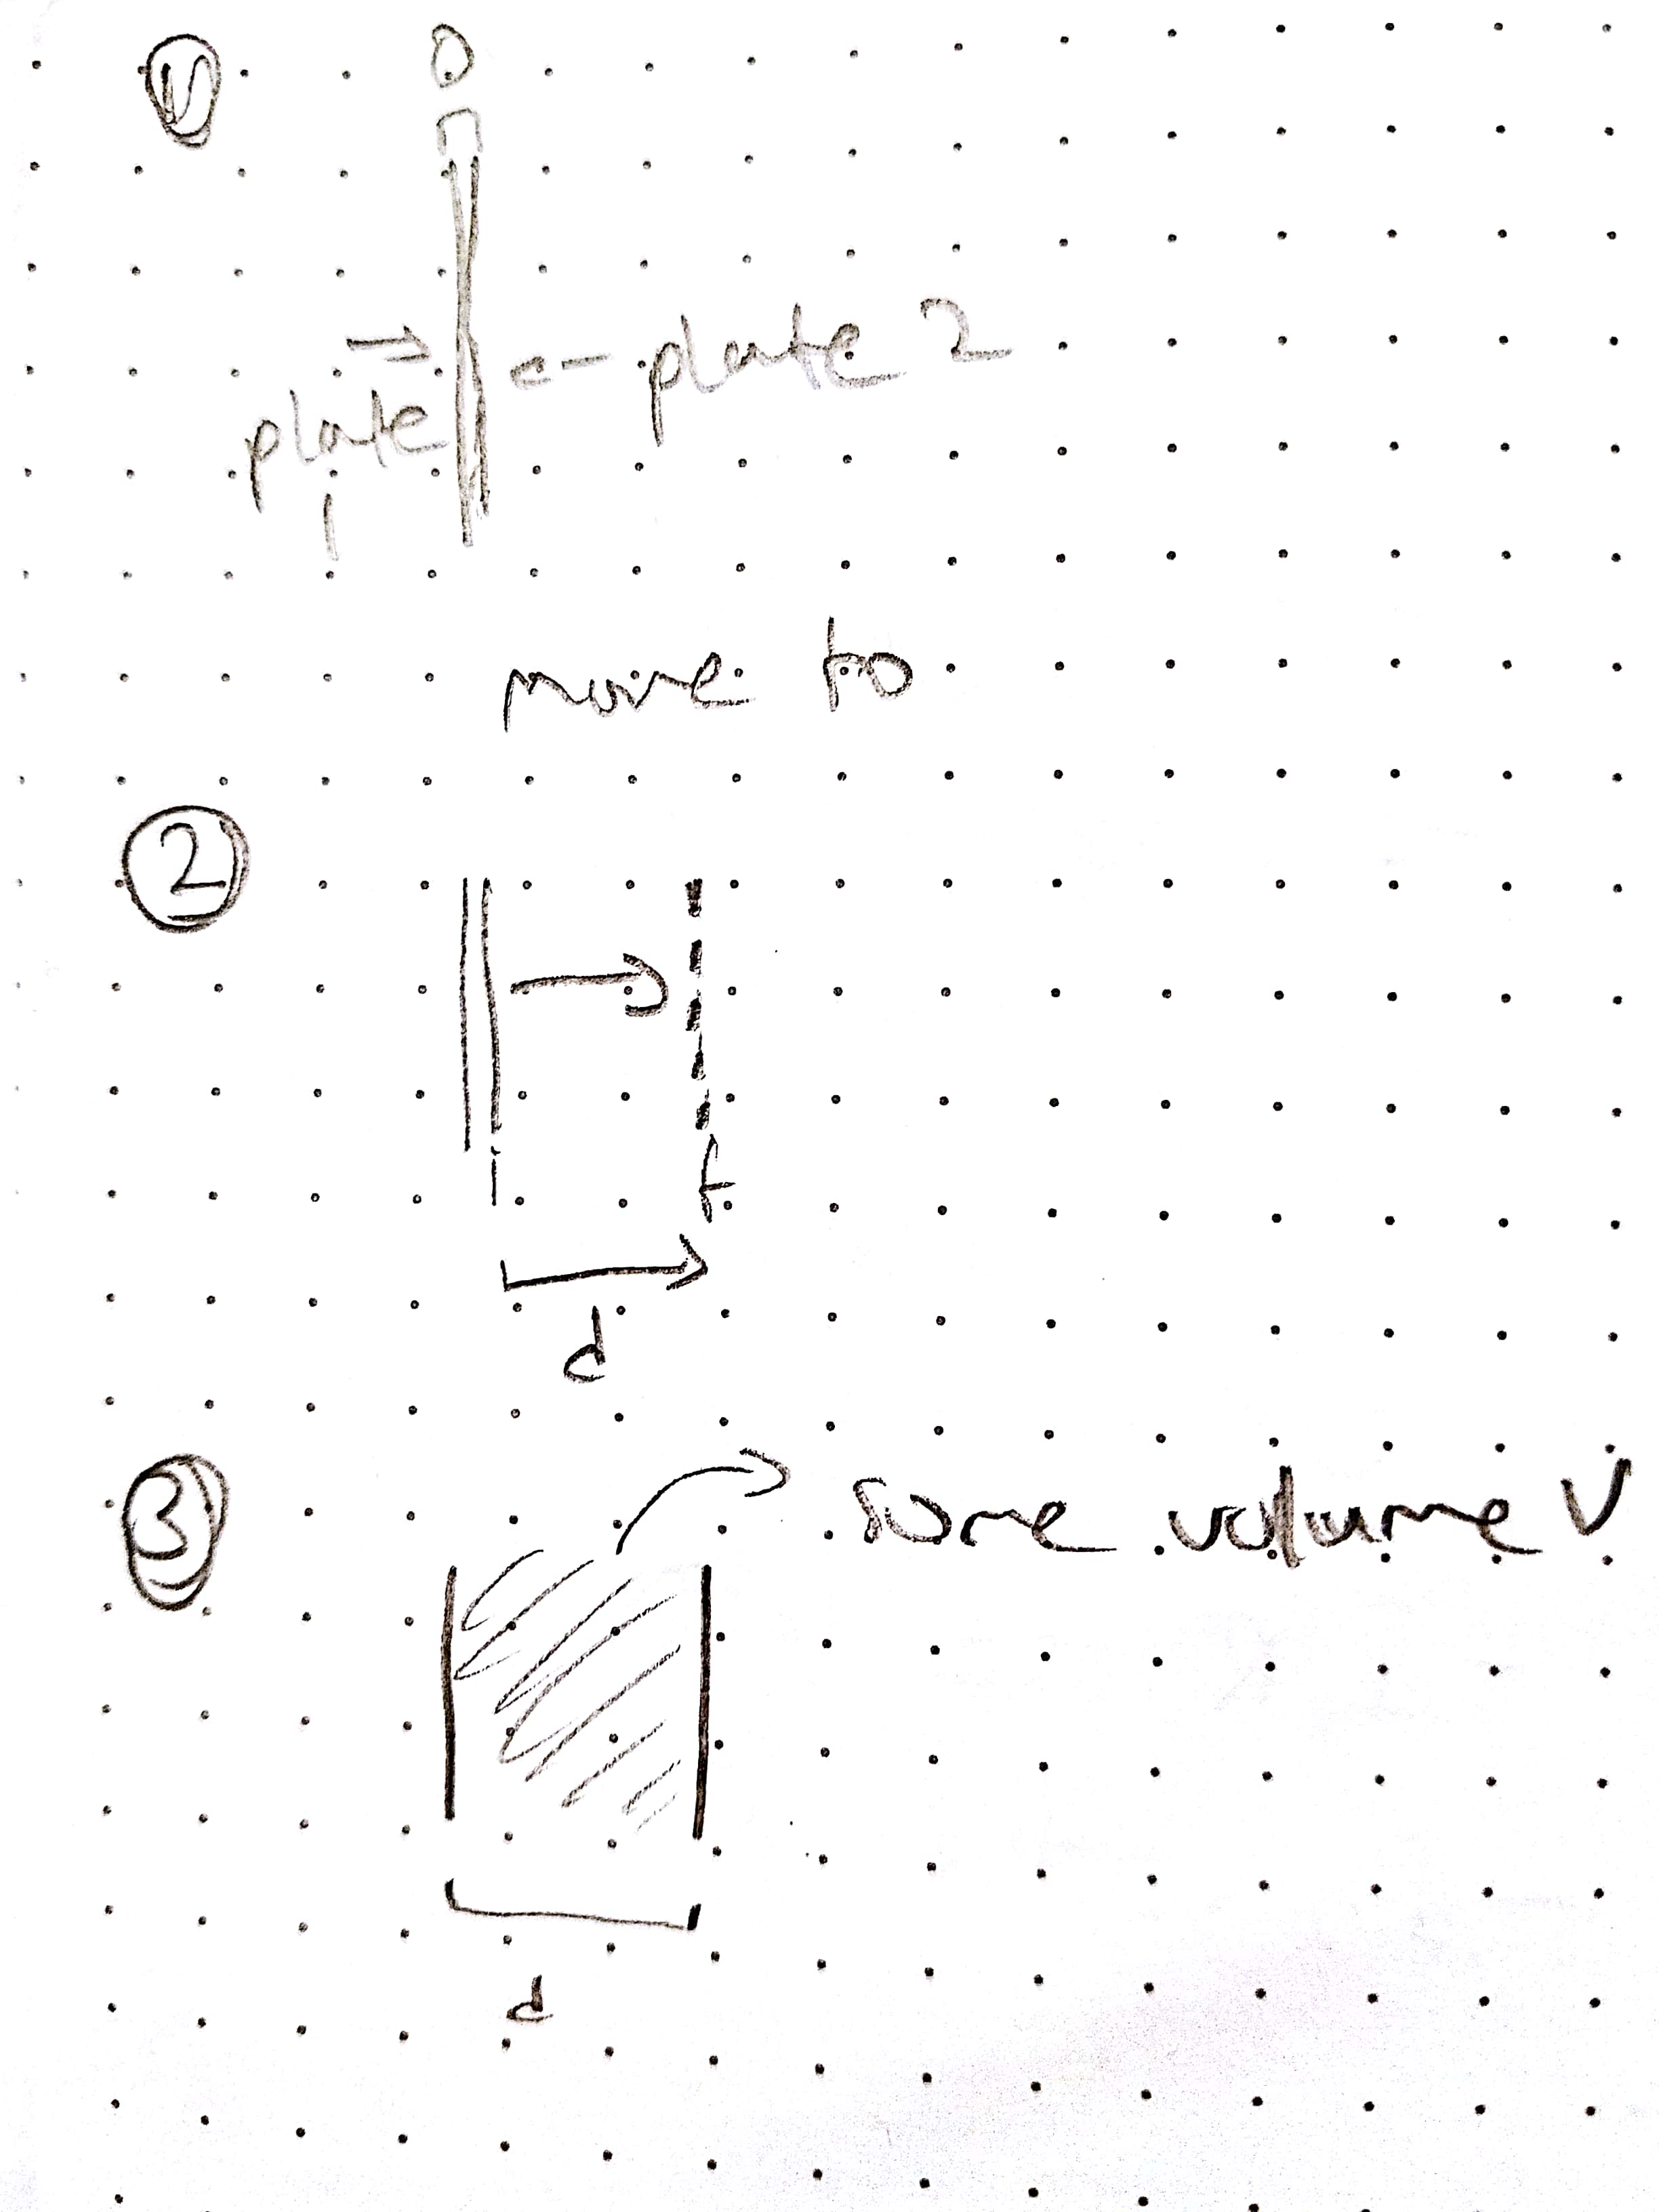
\includegraphics[width=.3\textwidth]{images/Week2pic4.jpg}
\caption{The image displays the intuition behind what I am trying to do to calculate energy density. Notice I move a plate to some distance and enclose some volume.}
\end{figure}

So, I need to start by representing the charge I will take: $$Q = \sigma A$$where $\sigma$ is the energy density of the large plates. Then, I want to calculate my energy change per volume: $$\Delta V = \frac{1}{V}\int_0^d \vec{F} \cdot \dif \vec{r} = \frac{1}{V}\int_0^d \sigma A \vec{E} \cdot\dif \vec{r} = \frac{1}{V}\int_0^d \sigma A \frac{\sigma}{\epsilon}\dif r = \frac{1}{V}\int_0^d \frac{\sigma^2A}{\epsilon}\dif r$$One question that may arise is that, if my volume changes as my distance changes, so the volume $V$ should not be able to be taken out: $\frac{1}{V}$. However, the argument for this is that I want to evaluate the energy density given a fixed point, not some arbitrary changing point. In addition, consider I did put $\frac{1}{V}$ in the intergal. This would be the same as saying, for every infinitesimal distance I cover, I want to multiply that by my force per that different volume. However, that means nothing, as this does not properly calculate energy, since it now depends on a variant volume enclosed. But, we know that for these plates, energy is linear. That is, since it has a constant electric field, it's simply $\frac{\sigma}{\epsilon}d$. Moving on, we want to now evaluate this integral and simplify: 
\begin{align*}
V(d)-V(0) &= \frac{1}{V}\frac{\sigma^2Ad}{\epsilon} - 0\\
&= \frac{1}{V}\frac{Q^2Ad}{A^2\epsilon}\\
&= \frac{1}{V}\frac{Q^2V}{A^2\epsilon}\\
&= \frac{Q^2}{A^2\epsilon}\\
&= \epsilon\frac{Q^2}{A^2\epsilon^2}\\
&= \epsilon(\frac{Q}{A\epsilon})^2\\
&= \epsilon|\vec{E}|^2
\end{align*}
There is one final factor to point out: This is essentially moving one plate involving the influence of both. If we want the energy density for any particular electric field (or one of them), we have to halve the final answer. Thus, the final expression for energy density is:$$\frac{1}{2}\epsilon|\vec{E}|^2$$
\noindent\rule{\textwidth}{1pt}
\\
\\
Now, with all the necessary components, we can delve more into capacitors. We define capacitance on the equation: $q = CV$. Because capacitance is $\frac{q}{V}$ and voltage of a capacitor is defined across the distance between the plates (call it $d$), capacitance is roughly $\frac{A\epsilon}{d}$. So, capacitance is a rough way of measuring how much charge can I store on a plate. In addition, because we can represent the potential across the capacitors by this equation, if you calculate the energy for every little charge (after all, there are two plates) on a plate (with the electric field, pick one plate to measure the energy stored. As if you move one from the first plate to its new position but then multiply by charge to get the energy).
\begin{align*}
\Delta E &= \int V \dif q\\
&= \int \frac{q}{C} \dif q\\
&= \frac{1}{2}\frac{q^2}{C}
\end{align*}
Finally, if you would like to derive capacitors in series or in parallel, think about what is going on. In series, you want to substitute a single capacitor for 2 capacitors. Thus, the voltage across the sum of both capacitors must be the voltage of your final capacitor: $\frac{q_1}{C_1} + \frac{q_2}{C_2} = \frac{q_{\text{eq}}}{C_\text{eq}}$. However, there is an important idea to note about series capacitors. In series, even if the voltage across capacitors may differ, since they are in series, they are supplied with the same current flow. Meaning, after $t$ amount of time, the same charge has reached both capacitors(i.e. been charged the same amount). Thus:
\begin{align*}
\frac{q}{C_1} + \frac{q}{C_2} &= \frac{q}{C_\text{eq}}\\
\frac{1}{C_1} + \frac{1}{C_2} &= \frac{1}{C_\text{eq}}
\end{align*}
The charging and discharging of capacitors will be covered in the loop section. 
\\ 
\\
Now we will discuss resistance and resistors. Resistance is essentially used to decrease the voltage in a circuit. In fact, a result of Ohms law is $V = IR$, where $R$ is resistance, measured in $\Omega$ (Ohms). However, how do we measure resistance? There is constant that is a given material property called resistivity. This can be measured. Let us derive that:
\begin{align*}
V &= IR\\
R &= \frac{V}{I}\\
&= \frac{V}{\rho |\vec{E}|\nu A}\\
&= \frac{V}{\rho \frac{V}{L}\nu A}\\
&= \frac{L}{\rho\nu A}\\
\end{align*}
Since $A$ and $L$ doesn't depend on the material, we can say resistivity $r$ is:
\begin{align*}
r = \frac{1}{\rho \nu} = R\frac{A}{L}
\end{align*}
Where $R$ is resistance. Before we briefly discuss resistors and finding an equivalent resistance, you should understand several concepts about circuits. In a conventional circuit, any charge that flows through must, by the loop rule, have a total change in voltage of $0$ when it returns to the point it started at. In addition, because of this, parallel circuits must have the same voltage drop over the parts that are parallel in order to maintain this rule. In addition, the current through each parallel portion must sum up to the current that leaves and enters the parallel portion. Below, I have illustrated the series of concepts and results of the loop rule:
\pagebreak
\begin{figure}[ht]
\center
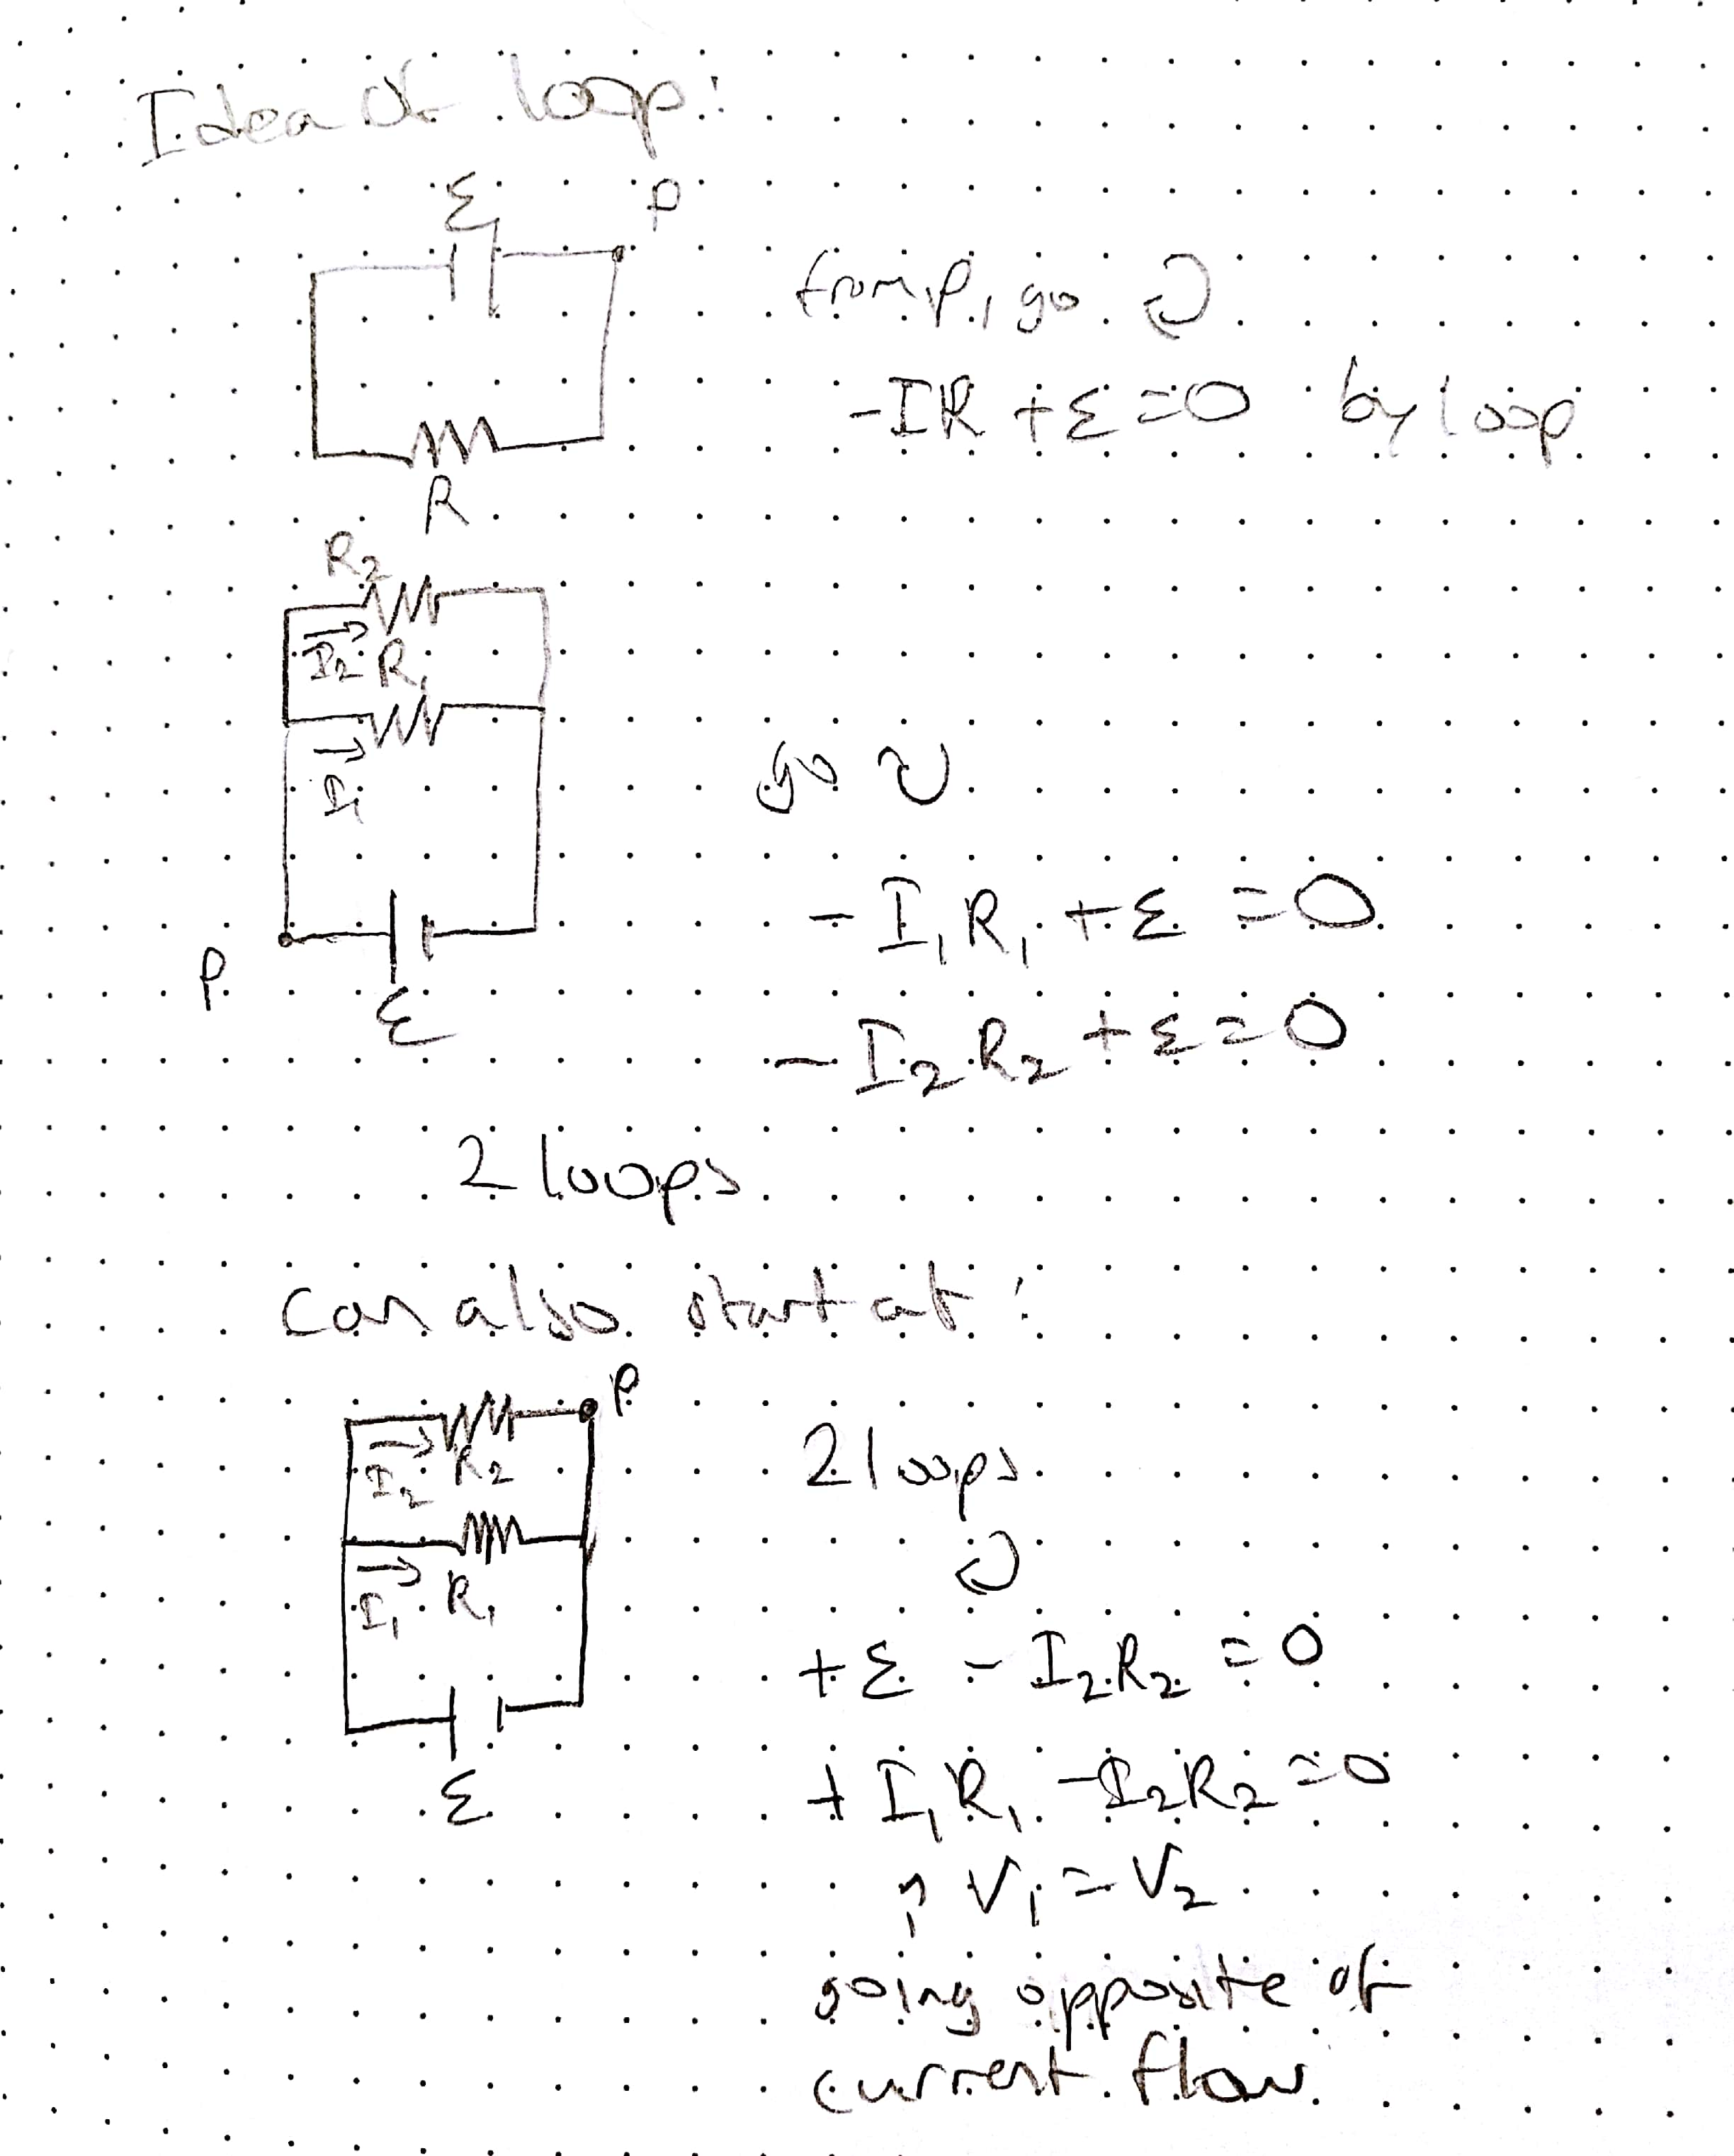
\includegraphics[width=.3\textwidth]{images/Week2pic5.jpg}
\caption{I have illustrated the loop rule above.}
\end{figure}
\\
When following the illustration, do note that when I choose a point, for simplicity sake, I can assume I have no initial voltage (as if I haven't passed through the battery yet). So I can start at $0$, but when I pass through the battery I gain voltage, when I go through a resistor, I lose potential. It's also important to note the loop where I only go around the parallel portion without the battery. This is fine, because what is a circuit really? The battery produces an emf that generates an electric field over the entire circuit. Imagine it like a vector field. We know that for all (that we will discuss) Coulomb fields, the field should be conservative, so it shouldn't matter what path we take. So instead of going through a part that gives me more potential, I can simply go in the smaller loop (through the parallel portion). All I'm doing is following the field and trying to reach the point I started at. This is also why my total change in potential from my starting point $P$ and going back to where I started is $0$. Remember, in a circuit, it's still as if you have a vector field, but it only exists along the circuit. But, we are always following the wires, so it's as if we are just in a vector field (don't forget this particular vector field is conservative!).  
%MIGHT ADD SECTION ON HOW BATTERIES ACTUALLY OUTPUT THE ELECTRIC FIELD INTO THE CIRCUIT BY FEEDBACK MECH%
It's very important to discuss capacitors with respect to the loop rule. Consider a capacitor, resistor, and battery in series. Let use write a loop rule to represent this. Choose some arbitrary point $P$, and the equation will still yield: 
\begin{align*}
+\varepsilon - IR - \frac{q}{C} = 0
\end{align*}
Before we go on, it is important to understand what we are trying to solve here. We want to solve for the charge on the capacitor as a function of time. We also know that $I$ is not constant since the capacitor causes the current to depend on time. Current is essentially $\frac{\dif q_i}{\dif t}$. However, this $q_i$ is the charge moving through the circuit. But, we know that $\frac{\dif q}{\dif t}$, where $q$ is the charge on the capacitor, is positive when the current is positive since the current charges the capacitor, then the equation is:
\begin{align*}
\varepsilon &= \frac{\dif q}{\dif t}R + \frac{q}{C}\\
C\varepsilon &= \frac{\dif q}{\dif t}RC + q\\
C\varepsilon - q &= \frac{\dif q}{\dif t}RC\\
\frac{\dif t}{RC} &= \frac{\dif q}{C\varepsilon-q} \\
\frac{1}{RC}\int_0^t \dif t &= \int_0^q \frac{\dif q}{C\varepsilon-q}\\
\frac{t}{RC} &= -\ln(C\varepsilon - q)\big|_0^q\\
-\frac{t}{RC} &= \ln(C\varepsilon - q) - \ln(C\varepsilon) \\
-\frac{t}{RC} &= \ln(\frac{C\varepsilon - q}{C\varepsilon}) \\
e^{-\frac{t}{RC}} &= \frac{C\varepsilon - q}{C\varepsilon}\\
C\varepsilon e^{-\frac{t}{RC}} &=C\varepsilon - q\\
q &= C\varepsilon - C\varepsilon e^{-\frac{t}{RC}}\\
q(t) &= C\varepsilon(1 - e^{-\frac{t}{RC}}) 
\end{align*}
Looking at the equation, we observe several important things. Firstly, as time approaches $\infty$, our charge on the capacitor is as we expected, $q \rightarrow C\varepsilon$, which also means that the voltage complete opposes the battery's voltage: $\frac{q}{C} \rightarrow \varepsilon$. At this point, we should also expect our current to be $0$, since we have two opposing voltages, which apply opposite electric fields. Another way of reasoning this is by the loop equation $\varepsilon - IR - \frac{q}{C} = 0$. If we had current but $\frac{q}{C}$ was $\varepsilon$, our loop would have a negative total voltage, which is not the case. Thus, $I \rightarrow 0$. You can also reason that because the current is also the rate of change of charge on the capacitor, taking the derivative of our derived equation and setting $t = \infty$ will yield $0$. After all, our capacitor is no longer charging as $t \rightarrow \infty$ as our capacitor's charge is constant as $t \rightarrow \infty$.\\
\\
Another important problem to solve is the discharge of a capacitor. That is, we have a capacitor, fully charged, as the power source. Let us solve the equation for a simple series circuit with just the capacitor and resistor. Choose a point $P$, and the general equation should follow:
\begin{align*}
\frac{q}{C} - IR = 0
\end{align*}
Now, we should once again think about what is $I$ in terms of the charge on the capacitor. We know that the capacitor's discharging gives us a positive current. However, a discharging capacitor has a negative $\frac{\dif q}{\dif t}$, since that is essentially the rate of change of charge on the capacitor, which lowers over time. Thus, the equation goes to:
\begin{align*}
\frac{q}{C} - (-\frac{\dif q}{\dif t}R) &= 0\\
\frac {q}{C} &= -\frac{\dif q}{\dif t}R \\
q &= -\frac{\dif q}{\dif t}RC \\
-\frac{\dif t}{RC} &= \frac{\dif q}{q} \\
-\frac{1}{RC}\int_0^t \dif t &= \int_{q_{max}}^q \frac{\dif q}{q} \\
-\frac{t}{RC} &= \ln(q) - \ln(q_{max})\\
-\frac{t}{RC} &= \ln(\frac{q}{q_{max}})\\
e^{-\frac{t}{RC}} &= \frac{q}{q_{max}}\\
q(t) &= q_{max}e^{-\frac{t}{RC}}\\
\end{align*} 
Similarly, we can see that as $t \rightarrow \infty$, the $e^{-\frac{t}{RC}} \rightarrow 0$. Howevever, rather than reaching a larger charge, we are discharging, as the equation converges to $0$ as $t\rightarrow \infty$. Now that we have covered capacitors, we should talk about energy and electric fields in circuits. Recall that in a conservative electric field:
$$-\oint \vec{E} \cdot \dif \vec{s} = 0$$
Let us apply this idea to the circuit. We can take out the portion due to the battery to get a general form for any circuit:
$$\varepsilon - \int_a^b \vec{E} \cdot \dif \vec{s} = 0$$
Where $a$ is the positive end of the battery and $b$ is the negative end. By this concept, let us consider a case where the entire circuit is just a constant wire of the same resistance everywhere. Then, clearly, $V = IR$. However, a more conceptual way of looking at this problem, which allows us to deal with the problem to more detail is to consider the electric field throughout the entire circuit. Because we must lose all our potential in order for our equation: $\varepsilon - b \int_a^b \vec{E} \cdot \dif \vec{s} = 0$ to hold true, we know that $\varepsilon = \int_a^b \vec{E} \cdot \dif \vec{s}$. This essentially says that the electrical energy expensed (notice how it's not a negative integral) should be the same magnitude as the potential energy. This is also the same as saying $\varepsilon + \Delta V = 0$, or change in potential over the circuit should be the same as the battery's potential gained. So, considering this form, let us go back to that wire and battery scenario. Because the wire is constant everywhere, we can argue that our potential should be distributed uniformly across the entire wire. $V_\text{per length} = \frac{\varepsilon}{L}$, where L is the length of the wire. However, we also know that $E = \frac{\dif V}{\dif l}$. Because we should have the same distribution of $V$ everywhere due to the wire's consistent resistance, the electric field is also:
$$E = \frac{\varepsilon}{L}$$
Thus, with any portion of the circuit with constant resistance, we can say that my electric field is just the voltage across that portion over the length of the wire. 
%ADD SECTION ON PUTTING DIELECTRIC IN BETWEEN CAPACITORS%

\pagebreak

\section{Week 3}
\subsection{Magnetism}
Magnetism is a very interesting field of physics. We generally know our simple bar magnets to have a North and South pole. If you may recall, opposite poles attract, and like poles repel. Later on, you will be able to understand why this is the case, and how to properly interpret bar magnets. We denote the magnetic field by the vector: $\vec{B}$. However, how do magnetic fields form? The magnetic field is generated by a moving charge. This is very important, as this will be the fundamental basis for many of our magnetic fields later. \\
\\
So, before we begin on discussing magnetic fields, we should first discuss the physical representation. The force on a charge that we are familiar with is the Coulomb force, which is an electrostatic force. However, there is another force, namely the magnetic force. However, an interesting result of observation and experimentation is that the magnetic force acts only on a moving charge. In fact, this force is always perpendicular to the direction of movement of the charge! So, by experimentation, we realize that our magnetic force does depend on these factors. The equation for the magnetic force on a charged object is given by:
\begin{align*}
\vec{B} = q\vec{v}\times\vec{B}
\end{align*}
\\
Notice that since the direction of magnetic force is perpendicular to the direction of motion, If you have a charge moving at constant velocity, as it turns, the magnetic force will still point perpendicularly, so the charge will actually go in circles. Thus, as you can see, magnetic fields can do no work on a particle. \\
\\
Moving along, just like the electric field, the magnetic field is a vector field. However, unlike electric fields, the magnetic field from any source (moving charge) will always be a ring of sorts, meaning the magnetic field will always be a sort of loop. This is due to the existence of magnetic dipoles. Now, as we said before, magnetic fields are generated by moving charges. This, as we'll discuss later, is due to changing electric fields. For a point charge, we can describe or magnetic field by:
\begin{align*}
\dif \vec{B} = \frac{\mu_0}{4\pi}\frac{q\vec{v}\times\hat{r}}{r^2}
\end{align*}
As our moving charge generates a mangetic field, a line of current will produce a very straightforward form for the magnetic field. We define the magnetic field for a line of current by: 
\begin{align*}
\dif \vec{B} = \frac{\mu_0}{4\pi}\frac{I\dif\vec{l}\times\hat{r}}{r^2}
\end{align*}
Once again, it is important to take a look at this equations to understand what they are trying to convey. Because these two equations are essentially the same, except one applies to a stream of charges, let us analyze the magnetic field equation for a point charge. Clearly, the charge has to be moving in order for a magnetic field to arise, as evident in the numerator. The equation also indicates a cross product with the $\hat{r}$, meaning it will always be perpendicular to the direction of movement and the radius vector to where I want to measure my magnetic field. Recall that this is $\hat{r}$, indicating direction. This cross product also means that I should have no magnetic field in the direction I am moving because my $\hat{r}$ and $\vec{v}$ will be in the same direction. In addition, once again, we have the inverse square relationship: $\frac{1}{r^2}$, similar to electric fields. So, the magnetic field weakens the further you get from the moving charge. So, how should I think about magnetic fields? A good way of thinking of magnetic fields from moving charges is a bunch of rings. Looking at the definition for our fields, we see that with any moving charge, the magnetic field is always perpendicular to the direction of movement and a radial vector. So, since we can construct infinitely many vectors radially at some radius, your magnetic field goes in a loop around the charge's movement. Because there are also infinitely many radii in space around the moving charge, every point in space has some magnetic field (including $0$) vector. This is also why we can define a magnetic field as a vector field as well. 

\pagebreak
\begin{figure}[ht]
\center
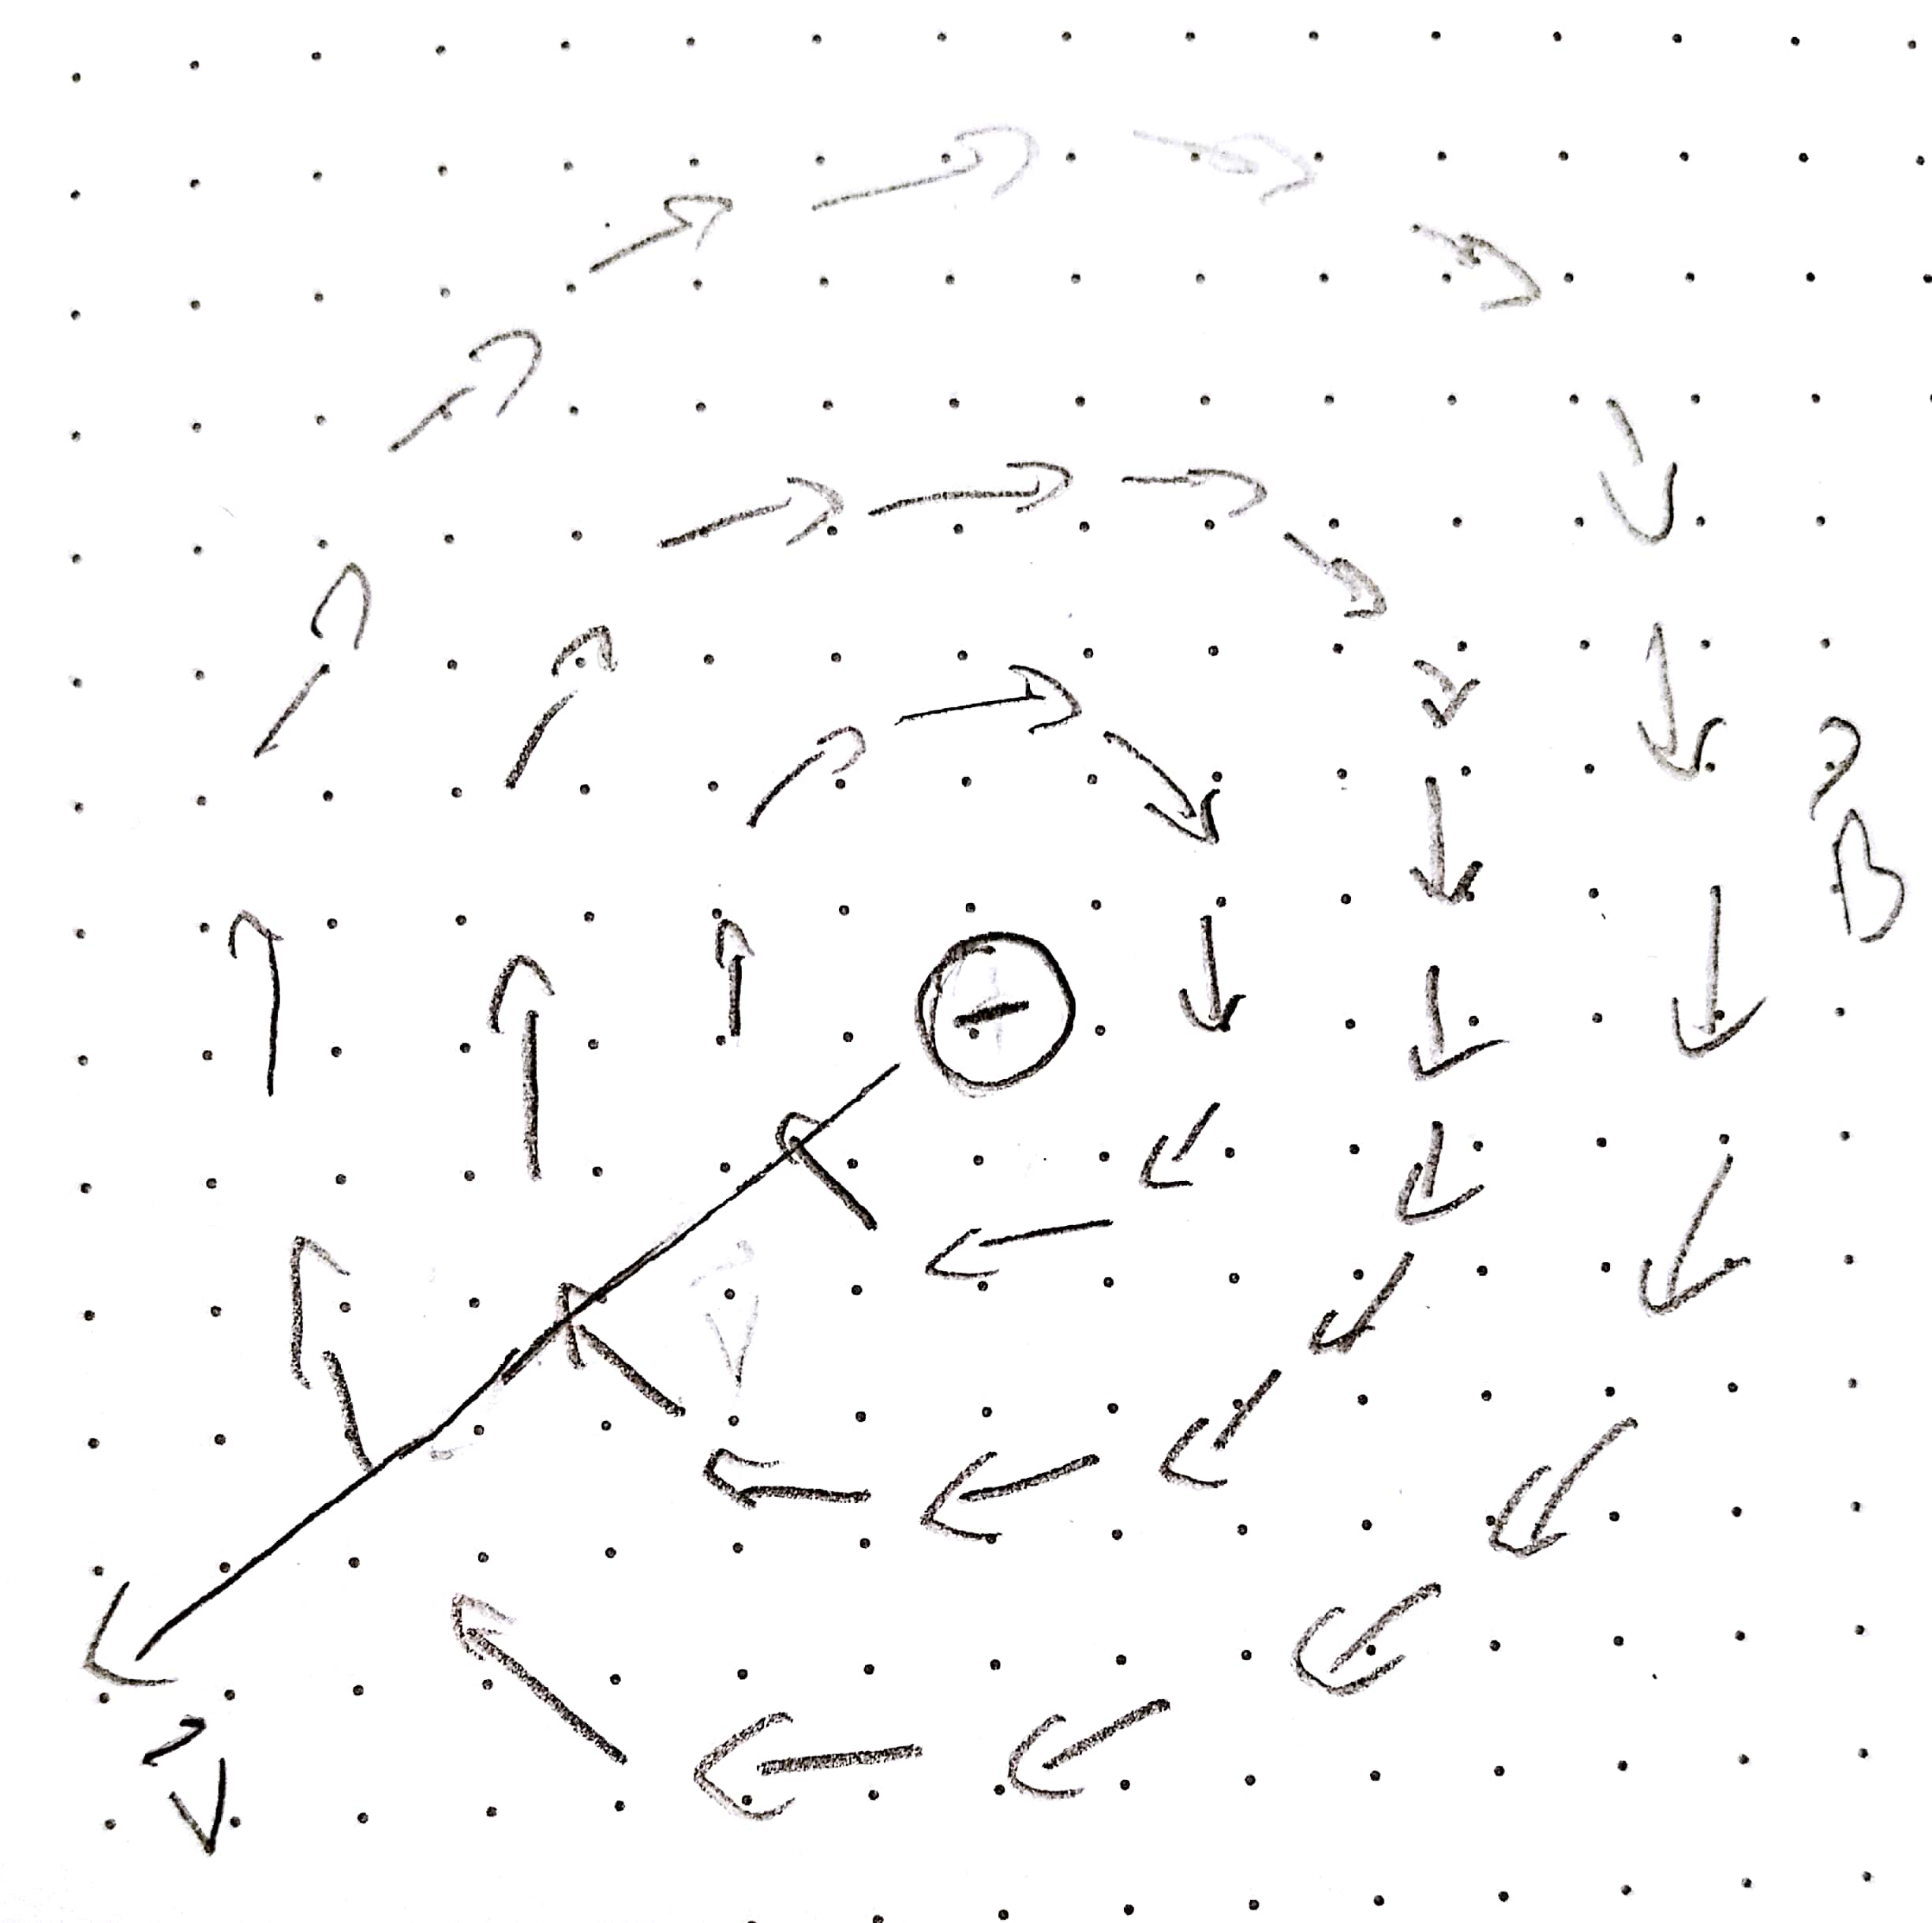
\includegraphics[width=.3\textwidth]{images/Week3pic1.jpg}
\caption{In the above image, note the magnetic fields going in circles. Do note that the magnetic fields I drew are only in the plane of the charge and vertical axis. There are magnetic fields everywhere in space, which should also follow the same loop direction. It goes clockwise because it's negatively charged.}
\end{figure}

Now that we have successfully understood the idea of the magnetic field, it is useful to actually determine a magnetic field. Let us work through a simple example. Consider an infinitely thin wire of uniform current $I$ where a piece of the wire of length $L$ is aligned along the x axis. We want to find the magnitude and direction of the magnetic field at the point illustrated below:

\begin{figure}[ht]
\center
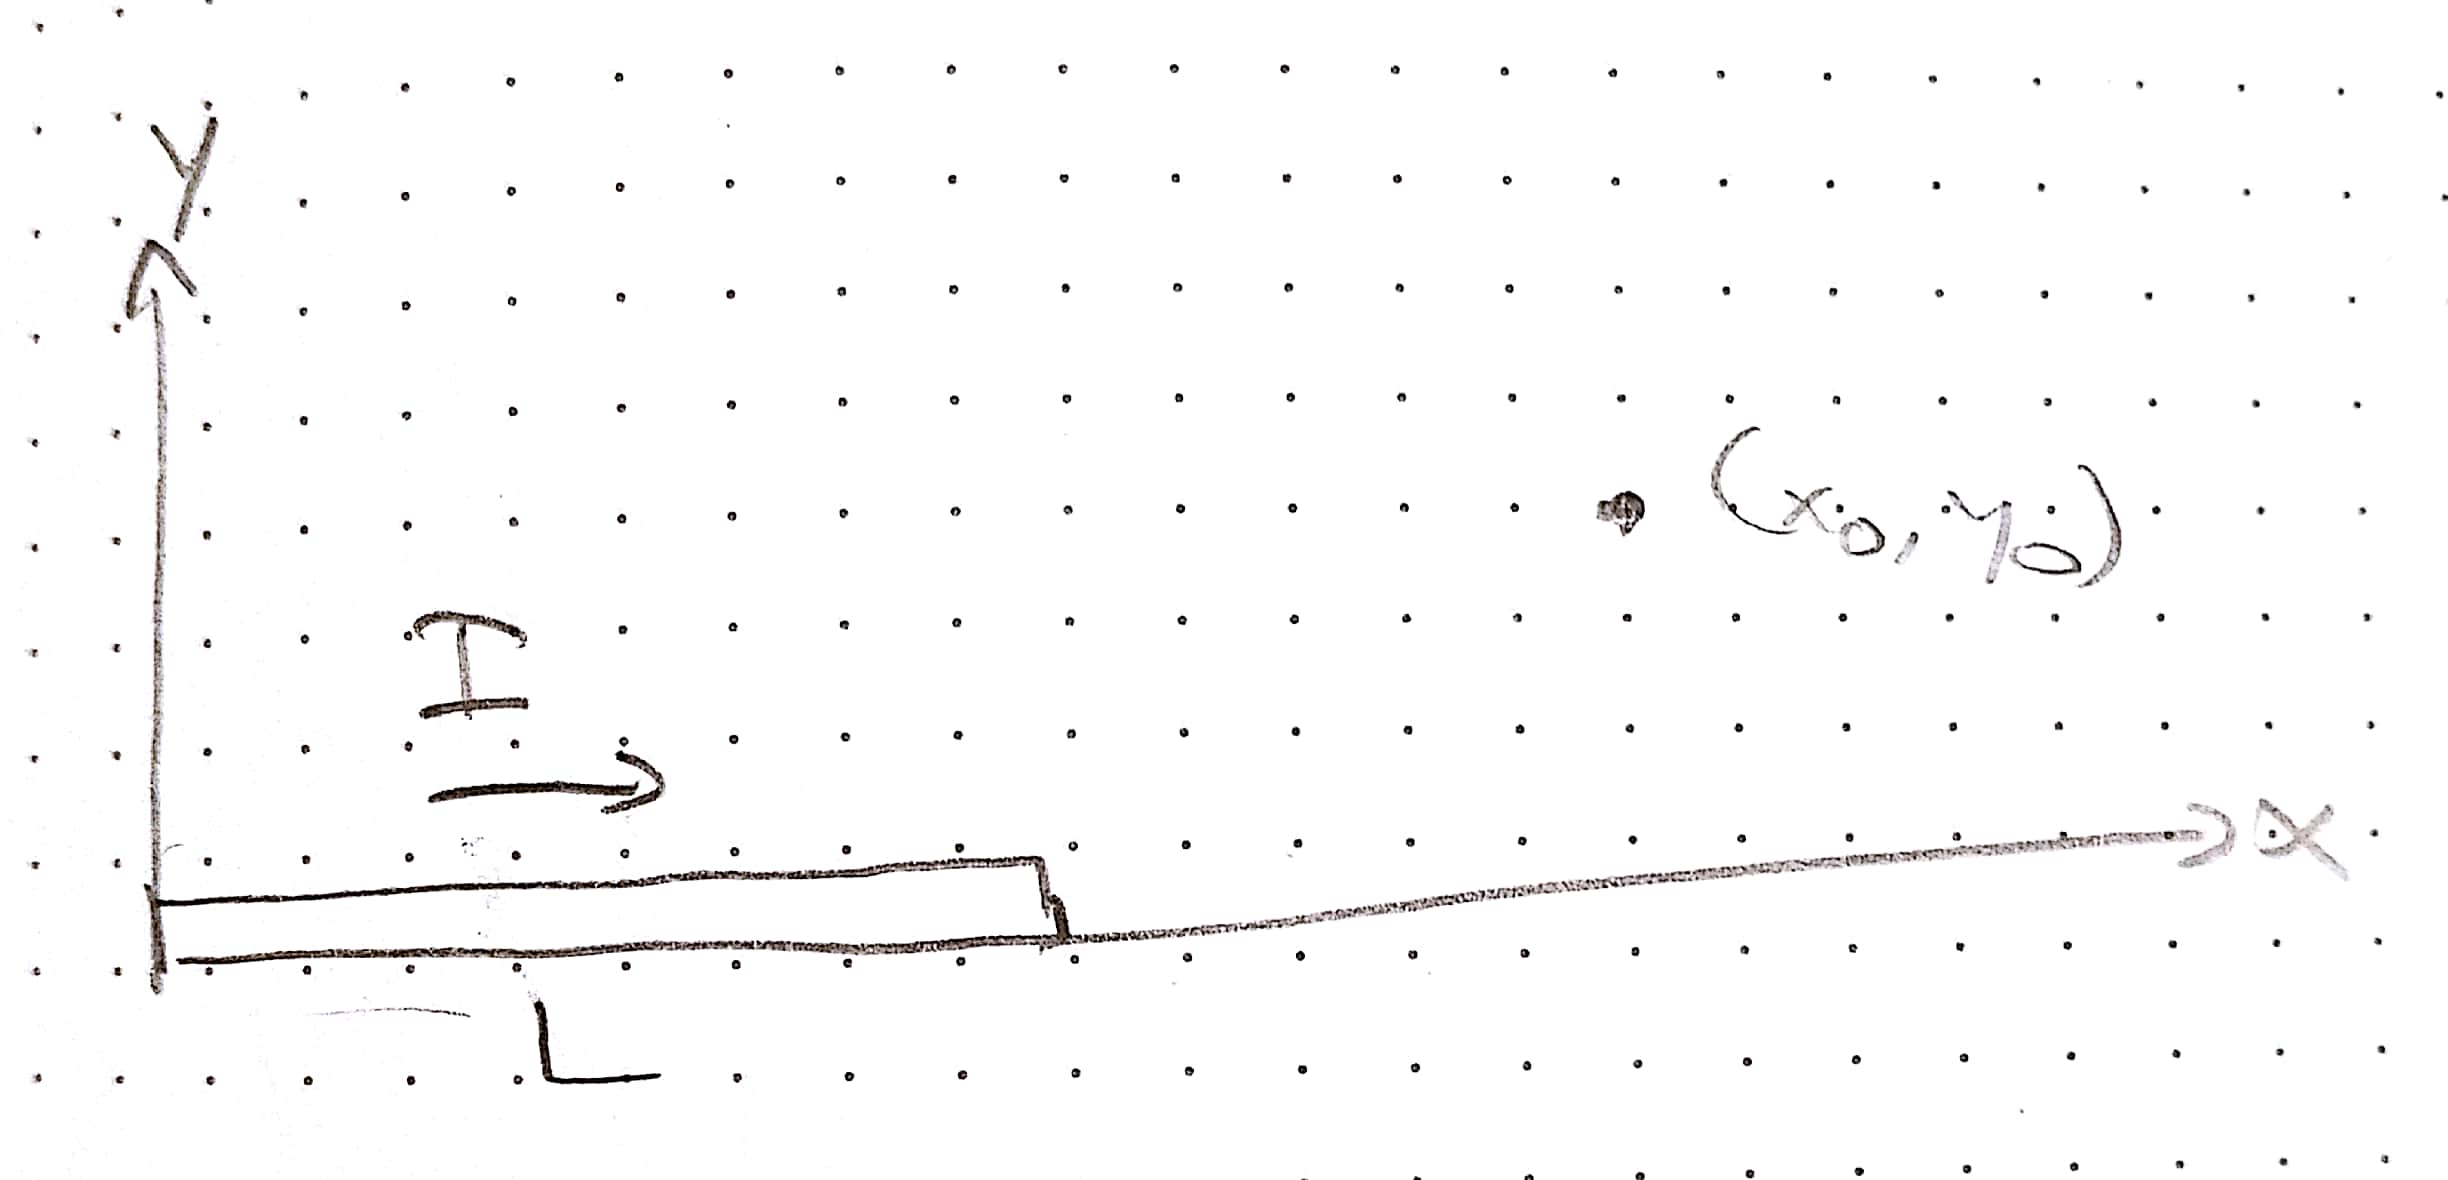
\includegraphics[width=.3\textwidth]{images/Week3pic2.jpg}
\caption{From the origin, we have the portion of the wire of current $I$. We want the magnetic field at the point ($x_0,y_0$)}
\end{figure}

To begin with, let us recall what the magnetic field definition means. First off, we have a current constant in the wire, meaning we can generalize our form of the magnetic field to the version that incorporates current: 
\begin{align*}
\dif \vec{B} = \frac{\mu_0}{4\pi}\frac{I\dif\vec{l}\times\hat{r}}{r^2}
\end{align*}

Primarily, we already have the differential form for us, as this describes each magnetic field contribution of each infinitesimal portion of the wire. However, in order to finalize the expression for integration, we must first define our $\vec{r}$ vector. Clearly, for each point on the wire, the vector pointing to the point $(x_0, y_0)$ is different. But, we can generalize this by describing the distance vector. To find this, take the difference between the positions. Let us define each point on the wire to be $(x,0)$.
\begin{align*}
\vec{r} &= (x_0, y_0) - (x, 0)\\
&= <x_0-x,\ y_0>\\
|\vec{r}| &= \sqrt{(x_0-x)^2 + y_0^2}
\end{align*}
Let us now rewrite our expression for the magnetic field. Note that our $\dif \vec{l}$ points along the x-axis:
\begin{align*}
\dif \vec{B} &= \frac{\mu_0}{4\pi}\frac{I\dif\vec{l}\times\hat{r}}{r^2}\\
&= \frac{\mu_0}{4\pi}\frac{I\dif\vec{x}\times\vec{r}}{r^3}\\
&= \frac{\mu_0}{4\pi}\frac{I\dif x <1, 0>\times <x_0 - x, \ y_0>}{((x_0-x)^2 + y_0^2)^{3/2}}\\
\end{align*}
We know that our x component of the $\vec{r}$ is $x_0-x$. However, notice we are doing the cross product. Since this is always parallel to the $\dif \vec{l}$ since they are both in the $\hat{x}$ direction, we only have the y-component, which is always perpendicular. Thus, our expression is simplified to:
\begin{align*}
\dif \vec{B} &= \frac{\mu_0}{4\pi}\frac{Iy_0\dif x}{((x_0-x)^2 + y_0^2)^{3/2}}\hat{z}\\
\vec{B} &= \frac{\mu_0}{4\pi}\int_0^L \frac{Iy_0\dif x}{((x_0-x)^2 + y_0^2)^{3/2}}\hat{z}
\end{align*}
So, in essence, the way to approach magnetic field problems is to think about what is being asked. In addition, you want to understand what it means to define the magnetic field via the general equation:
\begin{align*}
\dif \vec{B} = \frac{\mu_0}{4\pi}\frac{q\vec{v}\times\hat{r}}{r^2}
\end{align*}
In this case, we could simplify this to the current form because we were given that the wire had a uniform current. It is especially important to think about superposition. After all, we are describing the magnetic field at that point as each individual magnetic field from each infinitesimal part of the wire, all added up.\\
\\
Another important concept to go over briefly before going in depth (later on) is the idea of a current loop. We know that the magnetic field of any current is perpendicular to its direction. So, consider a loop of radius $r$ with a current $I$ going through it. Now, we want the magnetic field at the center. Since every $\dif \vec{l}$ is perpendicular to the $\hat{r}$, we can see that our expression for the field does not depend on the distance, since it is constant. Thus, our integration changes $\dif l$ to $2\pi r$. What's so important about the loop, however? Use the right hand rule and curl your fingers for every $\dif l$ of the wire loop. Notice that it all goes in the same direction in the center. On its own, this may seem pretty obvious, but the current loop is the definition of the magnetic dipole in the most simple way possible. In fact, this is approximately how magnetism works with atoms. In an atom, we have electrons orbiting the nucleus. Let us approximate the hydrogen atom to the planetary model. The electron orbits at a fixed radius. This results in a magnetic field. The reason most materials don't have an inherent magnetic field is simply because all the poles rearrange to cancel each other out. However, this is also why bar magnets exist. Every pole in the bar magnet is aligned in the same direction. Now, you may wonder: How would I perform calculations with a bar magnet? This is discussed later, but in essence, it is best to imagine the bar magnet as a current loop. Do note that you can construct any current loop you like, as long as it doesnt become discontinuous or zero (infinitely large or infinitely small). However, in construction, it is necessary to adjust the current and radius to compensate for each other, since when we say approximate as a current loop, we mean that it should carry the same magnetic field as the bar magnet.\\
\\
%Maybe use DiXiao's question of how to measure the mobile charges. People may think electric fields, but that fails because the electric force depends on the charge and the opposing directions will yield the same results. However, for a magnetic force, you can distinguish because they will yield differing results since the charges move in the same direction, which cause different fields
Let me bring up an interesting situation. Consider I have a magnetic field penetrating a bar of some material. In addition, let me say the mobile charges (free to move) in the bar are electrons, moving with some initial velocity $v$. Below I have drawn the situation. In this situation, I have connected the ends to a battery so the charges have some current $I$. 

\pagebreak
\begin{figure}[ht]
\center
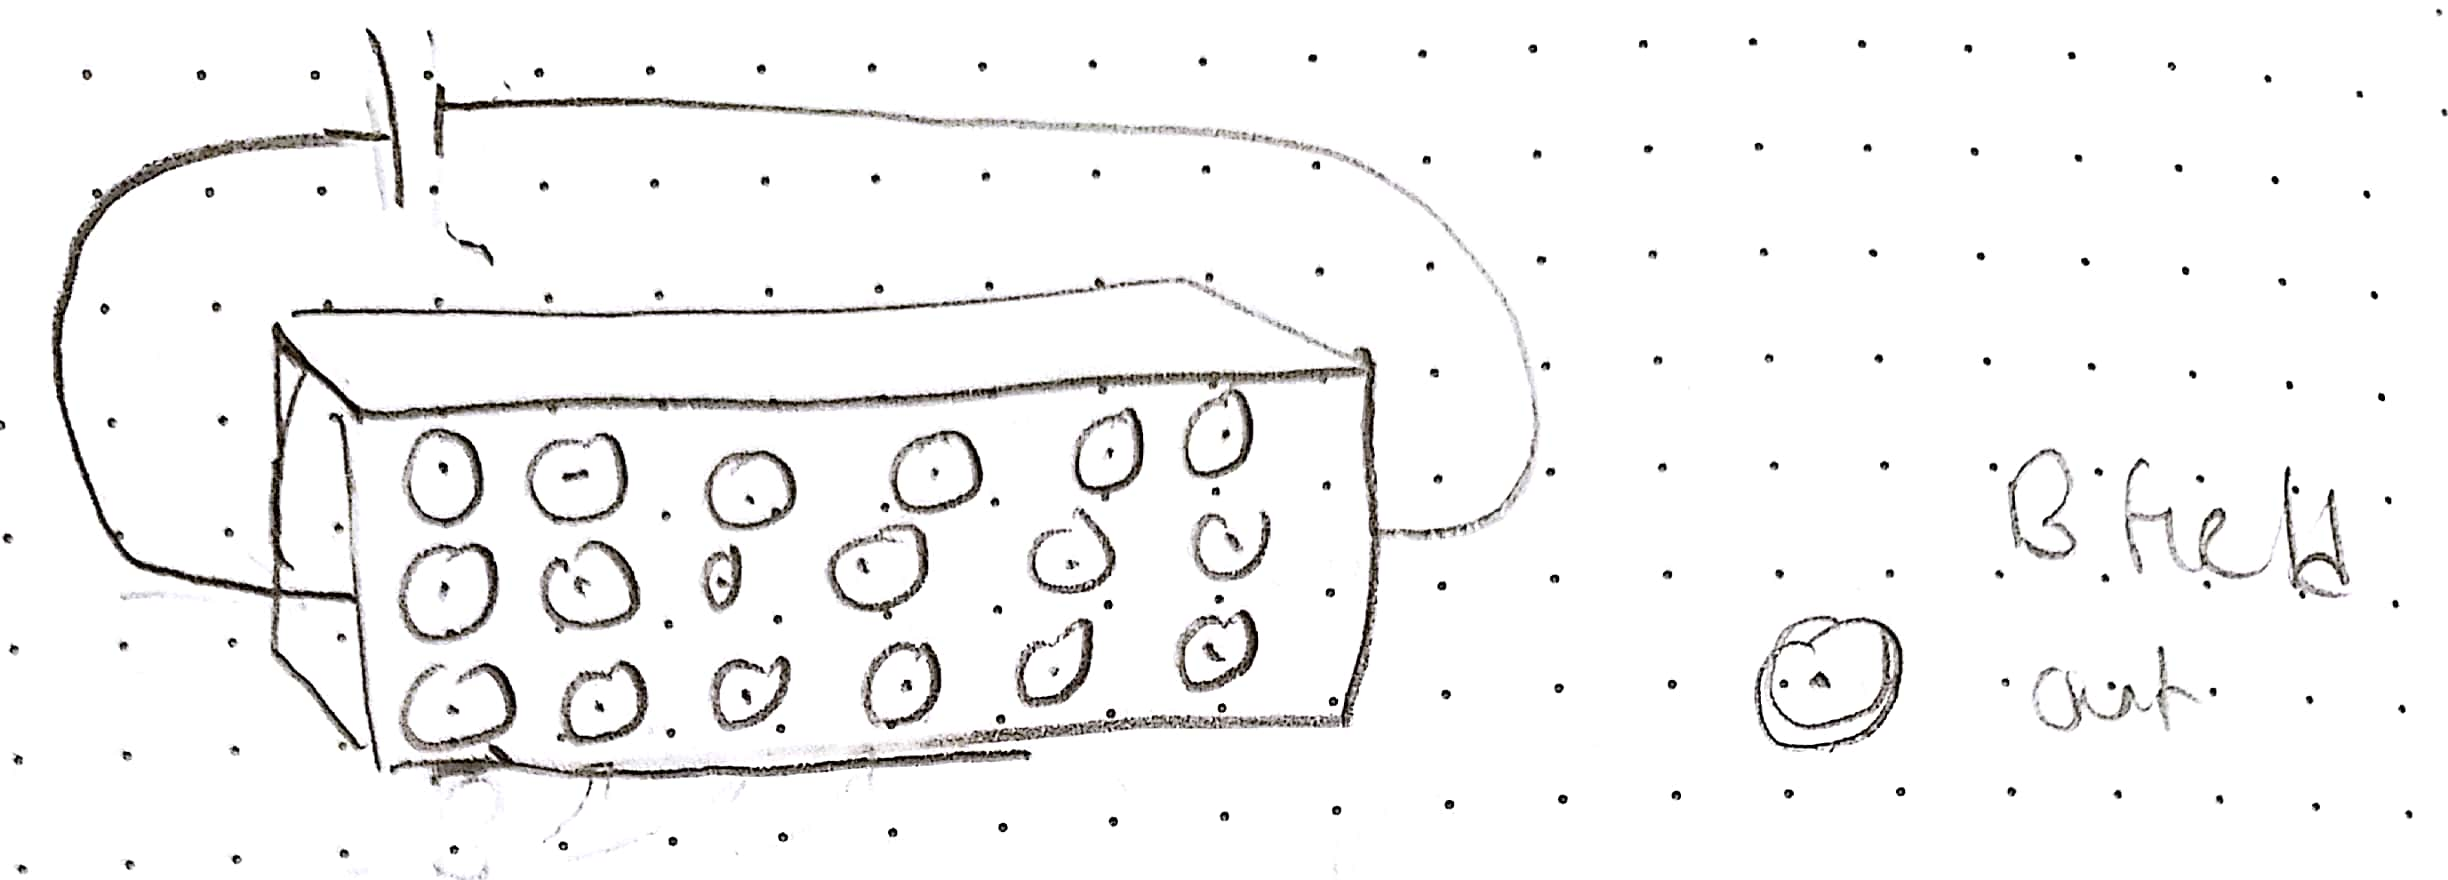
\includegraphics[width=.3\textwidth]{images/Week3pic3.jpg}
\caption{The image displays a battery applied to a bar. The magnetic field is pointing outwards.}
\end{figure}

Let us analyze this in a progressive time frame. Initially, the current is flowing from left to right. However, we have electrons as the mobile charges, so the electrons are moving from right to left. There is also a magnetic field pointing outwards too, so the magnetic force will push the electrons down towards the bottom. The negative charges will accumulate at the bottom of the bar. However, this also means a positive charge distribution is induced at the top, due to conservation of charge. What does this mean? This means, I have an elecrtic field pointing downwards. Let us analyze this further. If you notice, an electron moving in the bar now will feel the force from both the electric field and the magnetic field. As long as the magnetic force is stronger, the electron will move to the bottom. However, eventually, the accumulation of charge will yield an equally strong electric force. After all, Newton's first law says an object at rest will stay at rest unless an outside force is applied, which will compel it to move. In this case, the net force will keep moving the charges until the net force is $0$. Notice how this also demonstrates how nature always wants to reach equilibrium states. The effect of electrons moving and accumulating until there is an equal and opposite force is called the Hall Effect. The Hall Effect is extremely useful for several reasons. First, it allows us to determine what charges are mobile in a material simply by applying an electric field on either end and having a constant magnetic field. If you apply a voltmeter across the bar, the sign on the voltmeter will let you know where the charges accumulated. This is because regardless the sign of the charges, they will always move in the same direction, since their charge cancels out their opposing directions. \\
\\
\textit{Interesting Thought: Notice the very interesting nature of magnetic fields. If I had to try to determine the mobile charges with an electric field, this would not be possible. Consider any possible scenario. The electric field is defined by just the charge, causing the issue where the effect of the electric field will cancel itself out due to the charge. For example, apply an electric field on a metal bar. Yes, we eventually have no electric field inside, but regardless of what charge moves, you will have the same field induced. With a magnetic field, the field induced depends on the charge. The magnetic field works by being dependent on movement. In fact, this allows us to create separate situations.}\\
\\
The second reason why the Hall Effect is useful is because it acts as a speed filter. Any charge moving too fast or too slow will experience a force due to the magnetic field which will cause it to miss the exit. However, charges moving at the average velocity that caused the distribution will pass through. \\
\\
So, by understanding the concept of the Hall Effect, let us describe how we could find a relationship between the Hall Voltage (voltage induced by the effect) and both the magnetic field and voltage across the material (from the circuit). Let us also say the material has a length $L$, height $H$, thickness $W$, charge carrier density $n$, and resistance $R$. There are multiple ways to think of approaching this. First off, we can start with the given voltage across due to the circuit $V_0$ and solve for the voltage induced. We can also begin with the induced voltage $V$ and solve for the voltage across due to the circuit (which, we will choose). Then, let us start with the fact that the magnetic force and electric forces are equal and opposite after the charges have already accumulated. Then:
\begin{align*}
    \vec{E}q + q\vec{v}\times\vec{B} = 0\\
\end{align*}
However, we know that the electric field is roughly constant vertically because the material can be roughly approximated to be two large, charged, parallel plates. In addition, our velocity and magnetic field are perpendicular. So:
\begin{align*}
    \frac{V}{H}q &= qvB\\
    \frac{V}{H} &= vB\\
    V &= vHB\\
    V &= \frac{vHWB}{W}
\end{align*}
Now, let us say our charge carriers are positively charged (the sign is the only thing that changes), then they have charge $+e$:
\begin{align*}
    V &= \frac{nevHWB}{neW}\\
    &= \frac{BI}{neW}\\
    &= \frac{BV_0}{neWR}
\end{align*}
Do note that this is the relationship given the particular constants. It is purely a relationship, so depending on what you're given, certain constants can be substituted for more generalized constants. \\
\\
Now that we have thoroughly discussed fields (which we will return to later), it is also important to discuss magnetic forces in more detail. As we have seen, the Hall Effect is a direct effect of magnetic forces. Currently, our definition of the magnetic force for a moving point charge is $\vec{F} = q\vec{v}\times\vec{B}$. However, what if we had a piece of wire, which has moving charge? We can approach this by thinking of the superposition principle again. The force on the wire is the sum of all forces on individual charges. Thus, we want to sum up the effect on every infinitesimal charge $\dif q$. So, we can write a differential form for our force on a $\dif q$ charge: 
\begin{align*}
    \vec{F} = \int \vec{v}\times\vec{B}\dif q
\end{align*}
We can also rewrite this expression as:
\begin{align*}
    \vec{F} &= \int \dif q \frac{\dif \vec{l}}{\dif t} \times \vec{B}\\
    &= \int \frac{\dif q}{\dif t} \dif \vec{l} \times \vec{B}\\
    &= I\vec{l} \times \vec{B}
\end{align*}
Because for a current carrying wire, our current is in the same direction as $\dif l$, we can make the $\vec{l}$ the vector. In fact, many problems in the scope of this course focus on calculations on current carrying wires and magnetic fields. Let me bring up an interesting question. If I have a magnetic field penetrating a current loop, as in it penetrates it with a $90$ degree angle to the loop, What would be the net force on the loop? The net force would be the sum of all the forces on the loop. Look at the example below:
\pagebreak
\begin{figure}[ht]
\center
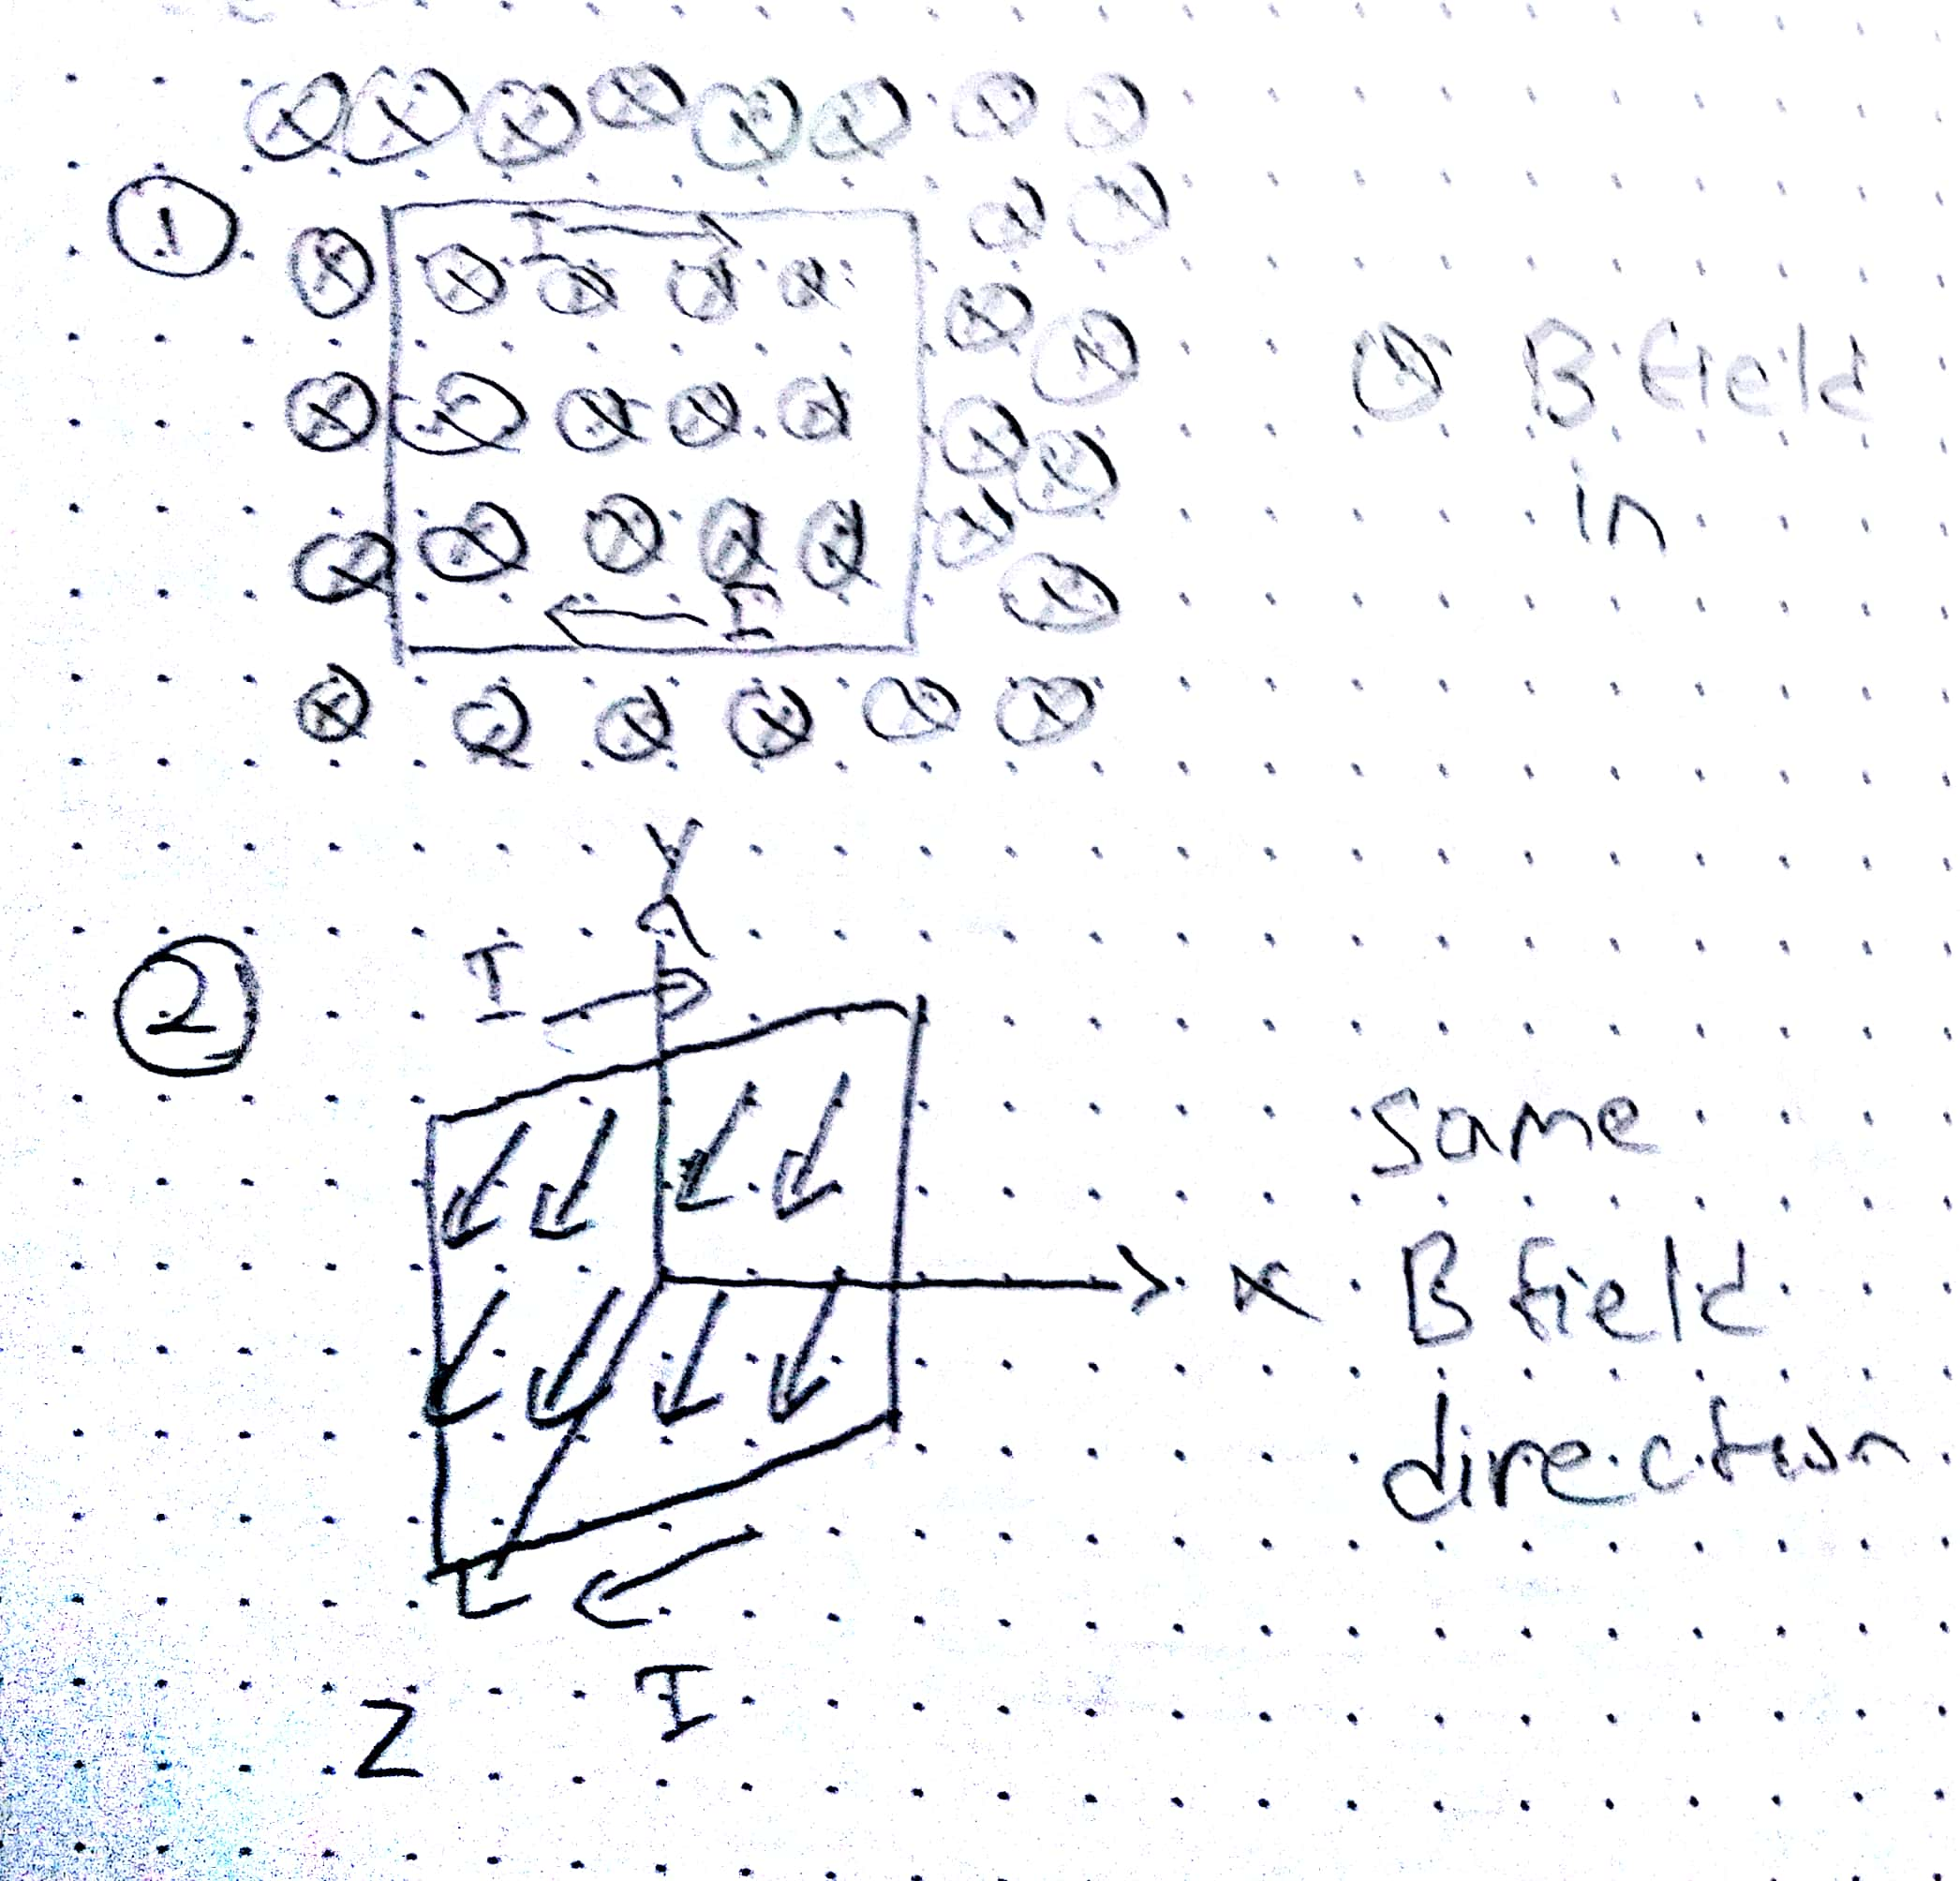
\includegraphics[width=.3\textwidth]{images/Week3pic4.jpg}
\caption{The image displays the magnetic field applied to a square loop of current in two different situations.}
\end{figure}


Analyzing each loop in ($1$), you can find out quickly that the force pushes outwards everywhere, so the vertical and horizontal components cancel out. However, let us rotate the loop a little so that the magnetic field penetrates the loop at an angle $< 90$ degrees, as we did in ($2$). Again, we have a constant magnetic field, so your current loop should still have a net force $0$. However, notice that while the net force is $0$, there exists a torque on the loop. After all, this is because our force vectors no longer lie in the same plane, but are parallel. This can also be understood as the fact that there exists a non-zero force component, decomposed orthogonal to the loop (One other way of understanding this is the fact that our vector from the center axis of the loop to the edge is no longer in the same direction as our force, which is how we define torque: $\vec{\tau} = \vec{r}\times\vec{F}$). This equation essentially is describing the force perpendicular to the axis of the rod ($\vec{r}\times\vec{F}$), multiplied by the radius from the axis of rotation ($\vec{r}$). Essentially, this can be re-represented more intuitively as: $\vec{\tau} = |\vec{r}|\hat{r}\times\vec{F}$ . So, let us calculate the torque on the loop:
\begin{align*}
\vec{\tau} &= \vec{r_1}\times\vec{F_\text{1}} + \vec{r_3}\times\vec{F_\text{3}}\\
\end{align*}
But, by our previous derivation, we know that the forces on each individual charge, summed up, can be expressed by $\vec{F} = I\vec{l}\times\vec{B}$, so this expression simplifies:
\begin{align*}
\vec{\tau} &= \vec{r_1}\times(I\vec{L_1}\times\vec{B}) + \vec{r_3}\times (I\vec{L_3}\times\vec{B})
\end{align*}
Now, before we represent the magnitude of the torque, we know that in the loop, the magnetic field is always perpendicular to the direction of $\vec{L_1}$ and $\vec{L_3}$ since the magnetic field is just pointing radially from the left and right vertical portions of the loop. In addition, because the directions of $r_1$ and $r_3$ are opposite and $L_1$ and $L_3$ are also opposite in direction, the ultimate cross product will be the same direction. Lastly, this loop is square, so $r = \frac{L}{2}$ and the sides are all perpendicular. Then, our magnitude of the torque condenses to:
\begin{align*}
|\vec{\tau}| &= I|\vec{r_1}||\vec{L_1}||\vec{B}|\sin{\theta} + I|\vec{r_3}||\vec{L_1}||\vec{B}|\sin{\theta}\\
&= 2I|\vec{r}||\vec{L}||\vec{B}|\sin{\theta}
\end{align*}
Be sure to understand that it doesn't matter what $r$ and $L$ I am using, since it should yield the same expression by the argument above, so I generalize it. Continuing:
\begin{align*}
\tau &= 2I\frac{L}{2}LB\sin{\theta}\\
&= IAB\sin{\theta}
\end{align*}
However, notice that through this expression, I can represent it using vectors by:
\begin{align*}
\vec{\tau} = I\vec{A}\times\vec{B}
\end{align*}
Where $\vec{A}$ depends on the direction of my current, since my area vector depends on the length vectors, which depend on the direction of the current (this is only true because we defined length vectors here that way. In other situations, it may be defined differently. However, if you read the previous derivation of the force on a line of current, it is more formally written as $\vec{F} = L\vec{I}\times\vec{B}$). 
Now, it's important to ask "Why?" as to why I can formally write torque this way. There are two ways of explaining this. Mathematically, work out the directions and also understand that the radial vector is perpendicular to the length vector everywhere for what we are concerned with. Another way of thinking about this is that because our directions are the same, we realize that the torque really depends on what my area looks like. So, we see that the same results would follow. This is essentially how we define the magnetic moment for current loops $\vec{\mu} = I\vec{A}$. However, the essential concept of the magnetic moment is that it is \textbf{defined} by the torque on a magnetic dipole by $\vec{\tau} = \vec{\mu}\times\vec{B}$.


%Talk about why bar magnetics are magnetic later on after discussing loop %


\pagebreak

\section{Week 4}
One of the most fundamental concepts that links electricity and magnetism is Faraday's Law of Induction. In fact, because it bridges the gap between electric and magnetic fields, it is incorporated as one of Maxwell's Equations. Faraday derived an expression that showed that the potential energy in a loop induced by a changing magnetic field depends on the rate of change of the magnetic flux. His expression essentially explains that a changing magnetic field induces an electric field. In fact, were you to move a bar magnet through space, along its path, there would be an infinitude of electric field loops surrounding it. You can think of it like how a current carrying wire generates magnetic field loops at every point radially. By definition: 
\begin{align*}
V = -\frac{\dif BA}{\dif t}
\end{align*}

However, it is very important to develop an intuitive understanding for why this is the case. While I do not have a strong enough explanation for how a time dependent magnetic field induces a voltage because it changes the magnetic flux, I can offer a strong argument to solidify the understanding for how, if the magnetic flux changes through changing its area, there is a voltage induced. Consider the scenario below:

%INSERT IMAGE%

\pagebreak

\section{Week 5}

\pagebreak

\section{Week 6}

\pagebreak

\section{Maxwell's Equations}
This section goes in depth in explaining the implications and intuitions for understanding and using Maxwell's Equations. First, I will write down the 4 equations governing electric and magnetic fields. Note: \textbf{Boldfaced} variables simply mean that they're vectors:
\begin{align*}
    \oiint_{\partial \Omega} \VF{E} \cdot \VF{n} \dif S
    &= \frac{1}{\epsilon}\iiint_{\Omega} \rho \dif V\\
    \oiint_{\partial \Omega} \VF{B} \cdot \VF{n} \dif S
    &= 0\\
    \oint_{\partial \Sigma} \VF{E} \cdot \dif \VF{s}
    &= -\frac{\dif}{\dif t}\iint_\Sigma \VF{B} \cdot \dif S\\
    \oint_{\partial \Sigma} \VF{B} \cdot \dif \VF{s}
    &= \iint_\Sigma \VF{J} \cdot \dif \VF{S} + \frac{\dif}{\dif t}\iint_\Sigma \VF{E} \cdot \dif \VF{S}
\end{align*}\\
\subsection{Gauss' Law for Electric Fields}

\begin{flalign*}
&\oiint_{\partial \Omega} \VF{E} \cdot \VF{n} \dif S = \frac{1}{\epsilon}\iiint_{\Omega} \rho \dif V&
\end{flalign*}

When we learn physics, we don't aim to just learn to utilize and memorize the equations. Rather, by understanding intuitively how the concepts are incorporated and how the different operators in the equation work together, you can understand exactly what is being modeled, which also allows you to be able to construct models for more situations.\\
With that being said, let us discuss Gauss' Law. The expression is very complex, but let us dumb it down to a very simple series of explanations. When we see a loop in the double integral, that means a closed surface integral. This is the same as saying: I want to find the flux through the entire surface (all faces). In the expression, we have $$\VF{E} \cdot \VF{n} \dif S$$Know that $\VF{n}$ is the unit vector pointing orthogonal (perpendicular) to the surface. In addition, when we do a dot product $\VF{E} \cdot \VF{n}$, we are saying what is the component of the electric field going perpendicular to the surface. This is multiplied by $\dif S$, or a small piece of area on the surface. So we can visualize this as similar to saying $$\VF{E} \cdot \dif \VF{A}$$which we know to be the definition of the electric flux. Then, the left hand side of Gauss' Law simply says: I want to calculate the entire electric flux through a closed surface. In Gauss' Law, this closed surface is the surface you construct. On the right side, we have $$\frac{1}{\epsilon}\iiint_{\Omega} \rho \dif V$$$\rho$ is our charge density, so by doing a triple integral over our surface, we are saying: What is the charge enclosed by our surface? So the main idea of Gauss' Law is that it relates the electric flux to the charge enclosed. Notice that to utilize Gauss' Law, you should know what the electric field looks like. This is so that you can know how to use ideas like symmetry to get a simple surface where the electric field goes through at a constant angle (hopefully perpendicular) and is constant. If it is constant, then the integral expression can be eliminated if you know the surface area of your surface. \\
\\
\subsection{Gauss' law for Magnetic Fields}
\begin{flalign*}
&\oiint_{\partial \Omega} \VF{B} \cdot \VF{n} \dif S = 0&
\end{flalign*}
Looking at the left side, this is simply the same expression for Gauss' Law for electric fields except replaced with magnetic flux. However, notice how the right hand side is 0. When we think about magnetic fields, we will always have loops. After all, unlike electric fields, magnetic fields always have a north and south pole, so the magnetic field cannot go off indefinitely without ever returning. As a result, when we talk about the closed surface integral, or the flux through the entire surface, we include both the magnetic field going out and the magnetic field coming back. These always cancel out (unless there are magnetic monopoles\footnote{Magnetic Monopoles are an active field of research. In fact, this version of Gauss' Law indicates that if there were monopoles, we would have a non-zero magnetic flux. There is no evidence to suggest that magnetic monopoles cannot exist.}), which leads to the 0.


%%%%%%%%%%%%%%%%%%%%%%%% MIGHT BE USEFUL TO INCLUDE A SECTION CONCEPTUALIZING FLUX BECAUSE IT IS AN ABSTRACT CONCEPT TO THOSE WHO HAVEN'T LEARNED IT. ALSO DISCUSS GRADIENT CONCEPTUALLY. %%%%%%%%%%%
\end{document}